\documentclass[letter,11pt,oneside]{report}
\usepackage[english]{swis_report_template}

%\usepackage{geometry} % Déinir les marges
\usepackage{latexsym,amsfonts,amssymb, amsmath, amsthm}

\usepackage{subfigure} % Plusieurs figures sur la même ligne.
%\usepackage{here} %positionnement H.
\usepackage{aeguill}  % sans ça, fontes bitmap affreuses Ruffin

\usepackage{fancyhdr} %Headers ++

\usepackage{ulem} % double soulignement

\usepackage{url} % Gestion des urls

\usepackage{pdfpages}

\usepackage[pdftex]{hyperref}
\hypersetup{
    bookmarks=true,         % show bookmarks bar?
    unicode=true,          % non-Latin characters in Acrobat’s bookmarks
    pdftoolbar=true,        % show Acrobat’s toolbar?
    pdfmenubar=true,        % show Acrobat’s menu?
    pdffitwindow=true,      % page fit to window when opened
    colorlinks=false,       % false: boxed links; true: colored links
    linkcolor=red,          % color of internal links
    citecolor=green,        % color of links to bibliography
    filecolor=magenta,      % color of file links
    urlcolor=cyan,          % color of external links
	pdfstartview = FitH, 	% La page prend toute la largeur
	pdfpagelayout = SinglePage, % Vue par page
	pdfpagemode = None, 	% Signets/vignettes fermé à l'ouverture
	bookmarksnumbered = true % Signets numérotés
}

%   
% bookmarks = true, 	% Signets
% bookmarksnumbered = true, 	% Signets numérotés
% pdfpagemode = None, 	
% %pdfstartview = FitH, 	% La page prend toute la largeur
% %pdfpagelayout = SinglePage, 	% Vue par page
% %colorlinks = false, 	% Liens en couleur
% %urlcolor = red, 	% Couleur des liens externes
% %pdfborder = {1 1 1} 	% Style de bordure : ici, pas de bordure
% ]{hyperref} 	% Utilisation de HyperTeX

%\addtolength{\textwidth}{0.7cm} %1.5
\addtolength{\textwidth}{2.8cm} %1.5
%\addtolength{\oddsidemargin}{-0.5cm}
\addtolength{\oddsidemargin}{-40pt} %-19
%\addtolength{\evensidemargin}{-19pt}
\addtolength{\marginparwidth}{15pt} % 11
\addtolength{\textheight}{60pt}
%\addtolength{\hoffset}{-1.5cm}  
\addtolength{\voffset}{-20pt}
%\setlength{\footskip}{0cm}

\newenvironment{my_itemize}{
\begin{itemize}
  \setlength{\itemsep}{4pt}
  \setlength{\topsep}{0pt}
  \setlength{\partopsep}{0pt}
  \setlength{\parskip}{0pt}
  \setlength{\parsep}{0pt}
}{\end{itemize}
}

\newenvironment{my_enumerate}{
\begin{enumerate}
  \setlength{\itemsep}{4pt}
  \setlength{\topsep}{0pt}
  \setlength{\partopsep}{0pt}
  \setlength{\parskip}{0pt}
  \setlength{\parsep}{0pt}
}{\end{enumerate}
}


\newtheorem{theorem}{Theorem}
\newtheorem{definition}{Definition}

%%
%%  Project details (please verify carefully with your project supervisor)
%%

\title{Hybrid Reactions Modeling for Top-down Design Framework}
\shorttitle{HyRToD Master project}
\author{Lo\"ic Matthey}
\semester{SS}
\year{2008}
\epflsection{IC-SIN}
\reportnumber{KUMAR-SWIS-MP12}
\startdate{19.02.2008}
\enddate{15.08.2008}
\professor{Alcherio Martinoli, Vijay Kumar}
\advisor{Gregory Mermoud, Spring Berman}
\coverimage{img/title.pdf}

% hauts de page
\pagestyle{headings} 
\markright{Lo\"ic Matthey }

%% 
%%  Title page, Table of contents, and running headers/footers are all 
%%  generated automatically (according to the information provided above, 
%%  and the structure of the document)
%% 

\begin{document}
\maketitle
\clearpage

% empty page
\pagebreak
\thispagestyle{empty}
\begin{center}\tiny \sc This page intentionally left blank.\end{center}

%% Project proposal
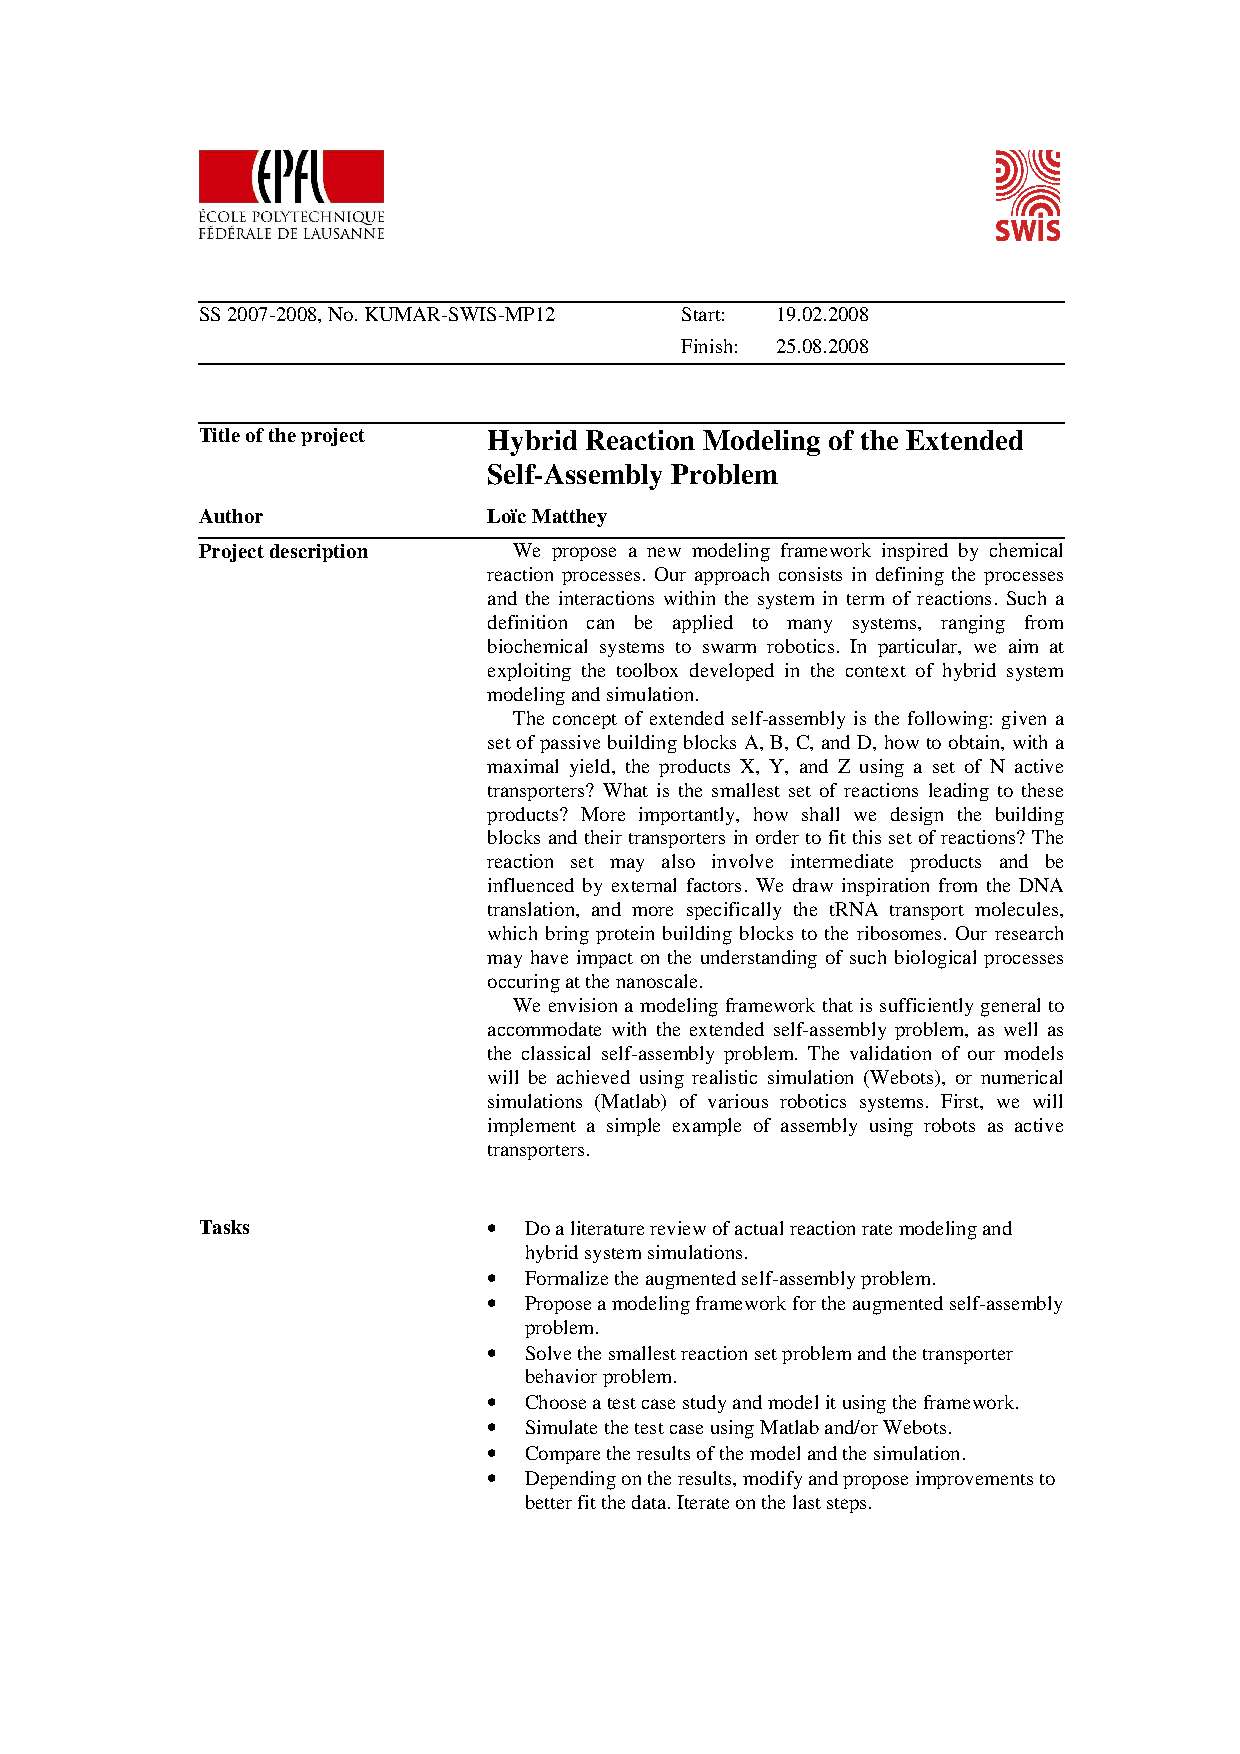
\includepdf[pages=1-2]{KUMAR-SWIS-MP12_proposal.pdf}

%%% Abstract %%%%
\begin{abstract}
	This report presents the work accomplished by Lo\"ic Matthey during his Master project from Ecole Polytechnique Federale de Lausanne (EPFL). This project was a joint work between the Distributed Intelligent System and Algorithms (DISAL) Laboratory at EPFL, Switzerland and the General Robotics, Automation, Sensing and Perception (GRASP) Laboratory at University of Pennsylvania, United States of America. It took place in the Master spring-summer semester 2008.

	We present a theoretical framework to design Top-down control scheme for arbitrary systems. Being able to control a complex system using high-level instructions only is a promising and attractive paradigm. Our approach is based on the use of a Chemical Reaction Network model, used as a proxy to derive the control schemes. To test the application of our method, we consider the Top-down control of a realistic multi-robots assembly platform, simulated using a 3D physics simulator, Webots.
	
	First we present the modeling of the robotic platform using a Chemical Reaction Network. The free parameters are precisely fitted. We simulate the system using an ODE approximation and an exact stochastic simulation. We find that the model can be made to fit quantitatively to the experimental data, especially when using a stochastic simulation approach.
	
	Second we define an optimization and control scheme for a class of Chemical Reaction Networks. We prove convergence results and write the optimization problem as a linear program of the time of convergence of the system under constraints on the equilibrium value. It allows us to design sets of reaction rates producing a specified converged behavior, in polynomial time. This optimization provides precise controls of the system using only high-level goals.
	
	Finally, we map the optimized model down onto the realistic physical assembly platform. We find that the system can be controlled using the optimized parameters of the model level, but that small discrepancies can have disruptive effects.

\end{abstract}

% empty page
\pagebreak
\thispagestyle{empty}
\begin{center}\tiny \sc This page intentionally left blank.\end{center}
\pagebreak

% List of figures
\setcounter{page}{1}
\setcounter{lofdepth}{2}
\listoffigures
% List of tables
\listoftables


\cleardoublepage
%%% Table of Contents %%%
\tableofcontents   % table des matières

% % empty page
% \pagebreak
% \thispagestyle{empty}
% \begin{center}\tiny \sc This page intentionally left blank.\end{center}
% \pagebreak

%%%%%%%%%%%%% Text %%%
%%
%%  Your report chapters begin here
%%


\chapter{Introduction} % (fold)
\label{cha:introduction}
	\section{Problem overview} % (fold)
\label{sec:problem_overview}

	Self-assembly is everywhere.
	
	\paragraph{}

	At every scale, systems interact, collaborate and combine to create new bigger scale systems. Crystals are formed by nanoscale assembly of carbon atoms, cell membranes by the arrangement of fatty acids into a lipid bilayer and human beings by the organization and cooperation of their trillions of living cells.

	Yet this process, being maybe so general and vast, is still tremendously unknown.

	The study of self-organizing systems gives insight into the organization patterns of their parts, and could help understanding and then modifying them.

	The recent field of Swarm intelligence applies the self-organizing principle to many systems and applications, ranging from algorithmic procedures (routing of packets, meta heuristics) to team of multiple robots. This approach makes sense when the number of robots increases to the point where a centralized or classical control methodology is not tractable anymore.
Interestingly, a similar problem occurs when the scale of robots and components starts to shrink down dramatically. If the environment is intrinsically random and unknown, the robustness factor promoted by self-organizing systems becomes a key factor.

	\paragraph{}
	Our interest goes towards that direction. We want to study systems whose dimension is shrinking to the level where classical approaches are not applicable anymore. Furthermore, we want to model those systems, and create a framework providing a complete control flow to modify the behavior of those systems.

	This might seem fairly trivial, but when the system under consideration is hard to study by definition and not well-known, even the simplest control over them or insight in their behavior becomes an appreciable achievement.

	\paragraph{}
	Our approach is the following:
	\begin{itemize}
		\item We propose an abstract way of describing the problem under study and the actions needed to achieve its control. Our main claim is that it is possible to divide the problem into two parts: an intrinsic system, on which we have no control, and an augmented system, which encompass our additions and modifications made to modify the behavior.
		\item We propose to use a Chemical Reaction Network mathematical framework through all this process to model the system under study. This framework will proves itself useful for its flexibility and expressive power at the scale we are studying.
		\item We present a way to control the system via a Top-down design approach, first working on the model and then mapping it back onto the studied system. Top-down design peaks the interest nowadays, as being able to control a complex system using high-level instructions only is a promising characteristic.
		\item Everything is presented and verified by referring to a specific system that we create and study: a robotic platform performing a self-assembly of products.
	\end{itemize}
	
	We call it the \textbf{Hybrid Reactions Modeling for Top-down Design Framework} (HyRToD). ``Hybrid'' because we will use both ordinary differential equations approximations and stochastic simulations to simulate the model, depending on the context.
	
	The robotic platform is actually simulated on a computer, by using a realistic 3D physics simulator named Webots~\cite{Michel:2004p10762}. Webots is based on ODE, an open source physics engine for simulating 3D rigid body dynamics~\cite{ode}. Such a simulator allows us to performs systematic experiments faster than real-time and with null fabrication costs.
	
	This might seems strange to apply a framework we claim to be thought for micrometer scale dynamics onto a high level robotic platform. We actually design the robotic platform to give it characteristics usually shown at a smaller scale, and therefore only take advantage of the robotic platform as a model system easy to measure and modify. This work focuses on this robotic platform as a first test for our framework. Further works will consider smaller scale applications to assess our initial assumption on our framework.
	
\subsection{Relations to biological processes} % (fold)
\label{sub:relations_to_biological_processes}
	Even though we apply our method to a robotic implementation, a fairly high scale system by all means, we claim that this method is applicable to many different systems, especially the ones governed by random dynamics.
	
	We chose to create a robotic platform performing a self-assembly task on purpose. Having robots carrying the building blocks and assembling them can be thought of as an idealization of the self-assembly process taking place into the cell, for example the protein synthesis. If we allow the building blocks to move around and assemble on their own, the added robots will behave like enzymes, promoting some reactions.
	
	Moreover, our method, using a Chemical Reaction Network model, is very easy to apply on biological processes. This model has been extensively used in the study of biological systems, and is very well understood by the community working in this field. This is an added factor to the development of further interdisciplinary cooperations between engineering and life sciences.
% subsection relations_to_biological_processes (end)


% section problem_overview (end)

\section{Outline} % (fold)
\label{sec:outline}
	This report is organized as follows: Chapter~\ref{cha:project_description} defines precisely our goals and the abstract problem definition and control flow we aim to study. Chapter~\ref{cha:field_overview} goes over the theoretical notions used in our work, and gives pointers to the available literature on the subject. Chapter~\ref{cha:puzzle_test_case_implementation} presents extensively the specific system we are studying, namely the physical robotic simulation of an assembly task. Chapter~\ref{cha:mathematical_model_of_the_puzzle_test_case} introduces the representation of our specific system into a Chemical Reaction Network notation, presents how we fitted the free parameters and compare the simulated results with the physical measurements. Chapter~\ref{cha:chemical_reaction_networks_control_and_design} is dedicated to the optimization step applied on our mathematical model in order to control its behavior. Chapter~\ref{cha:augmented_assembly_implementation} presents the Top-down mapping of the modified model towards the physical system. Chapter~\ref{cha:conclusion_and_outlook} concludes the work and assess its validity and shortcomings.
% section outline (end)
% chapter introduction (end)

% % empty page
\pagebreak
\thispagestyle{empty}
\begin{center}\tiny \sc This page intentionally left blank.\end{center}
\pagebreak


\chapter{Project description} % (fold)
\label{cha:project_description}
	%description: Project definition of the Puzzle test-case

\documentclass[letterpaper, oneside]{article}

\usepackage[utf8]{inputenc} 
							
\usepackage[T1]{fontenc}

\usepackage{graphicx} % images
\usepackage{geometry} % margins
\usepackage{latexsym,amsfonts,amssymb, amsmath, amsthm}

%\usepackage{subfigure} % several figures
\usepackage{aeguill}  % bitmap fonts ©Ruffin

\bibliographystyle{plain}

%\frenchspacing

\title{Stochastic assembly: a puzzle test-case}
\date{\today}

\newcommand{\loic}{Loïc Matthey}
\newcommand{\spring}{Spring Berman}

\author{\loic \and \spring} 

\pagestyle{myheadings} 

% headings
\markright{\loic \ and \spring}

%\addtolength{\textwidth}{1.5cm}
%\addtolength{\hoffset}{-1.5cm}  
%\addtolength{\voffset}{-1.5cm}
%\setlength{\footskip}{0cm}

\begin{document}


%\landscape
\maketitle

% \vspace*{2pt}
% 
% \begin{center}
% \begin{Large}
% 	\textbf{Computational Molecular Biology}\\
% \end{Large}
% \vspace*{5pt}
% \begin{large}
% 	Homework \#7
% \end{large}
% 
% \vspace*{3pt}
% 
% \aut
% 
% \end{center}

%\tableofcontents   % table des matières
%\setcounter{section}{1} 

% Content
\section{Problem description} % (fold)
\label{sec:problem_description}

\subsection{Complex System Modulation problem (Loïc's thesis)} % (fold)
\label{sub:underlying_problem}
Consider an intrinsic complex system with observable dynamics and a measurable performance metric. Let this intrinsic system attains an optimal performance metric value $X_{opt}$. Introduce agents into the system with designed specific behaviors, getting an augmented system. Can we design such behaviors so that the performance metric of the augmented system attains an optimal value $Y_{opt}$, with $Y_{opt} > X_{opt}$?
% subsection underlying_problem (end)

\subsection{Puzzle test-case} % (fold)
\label{sub:puzzle_test_case}

Consider the following task:
\begin{itemize}
	\item Let a puzzle of square shape, with area $5*5$, be constructed out of 5 pieces of area 5 each with different given shapes.
	\item Let the final assembly shape $S$ of this puzzle be know.
	\item Let the set of assembly plans $P$ leading to the final shape $S$ be known. 
	\item Let the puzzle pieces assemble by bi-directional connections. One connection is enough for two pieces to be attached. These connection and their positions on the different pieces are known.
	\item Pieces can be assembled and disassembled.
	\item Consider an arena of sufficiently large size so that small scale interactions dynamics can be ignored.
	\item Fill this arena with $N$ initial pieces of each shape.
	\item Consider $M$ robots, able to pick up pieces and to make them assemble and disassemble.
	\item Allow a recognition by the robots and by the pieces of the shapes and connection points when an encounter occur.
	\item \textbf{Then:}\\
	How can you manipulate those initial pieces so that after a time $T_f$, the number of assembled puzzles $X_S$ is maximized?
\end{itemize}

Consider two approaches for the robots behaviors:
\begin{enumerate}
	\item Stochastic interactions.
	\begin{itemize}
		\item The robots move randomly around the arena while carrying pieces.
		\item They can not communicate outside of collision radius.
		\item They know nothing or very little about the final assembly shape $S$ and the assembly plans $P$.
		\item Assembly and disassembly of pieces is random, according to specific probabilities depending on the pieces. These probabilities can be influenced by the knowledge of the final assembly shape $S$ and assembly plans $P$ if available.
	\end{itemize}
	
	\item Deterministic control-oriented.
	\begin{itemize}
		\item The robots move according to specific movement patterns.
		\item They can communicate outside of collision radius, in a local range $R$.
		\item They know completely about the assembly plans $P$ and the final assembly shape $S$.
		\item They assemble and disassemble pieces according to their local knowledge of the environment and their internal knowledge.
	\end{itemize}
\end{enumerate}

\subsubsection{Goal of test-case} % (fold)
\label{ssub:goal_of_test_case}
Compare the behavior of the two controllers with respect to the final number $X_S$ of assembled puzzles.
Assert under which conditions the two different approaches are more interesting.

Classical directions for the comparison can be:
\begin{itemize}
	\item Level of error in the system. Typical errors: bad assertion of pieces shapes and type, bad communication between errors, bad assembly of pieces, unknown initial conditions.
	\item Complexity level of the robots and pieces. Typical capabilities: global positioning, computing power, communication range.
\end{itemize}
% subsubsection goal_of_test_case (end)

\subsubsection{The assembly line problem} % (fold)
\label{ssub:the_assembly_line_problem}
\begin{itemize}
	\item If we can control everything in our system, i.e. the level of error is almost zero, then why use stochasticity? More precisely, why disassemble things and not use the perfect assembly plan?
	\item If we are at a high enough level of complexity, then classical deterministic methods which act optimally are obviously better.
	\item Situations where this is not true anymore:
		\begin{enumerate}
			\item There is intrinsic stochasticity in the process, or we cannot control it completely. Examples: self-assembly at small-scale, which stochastic dynamics.
			\item The agents make errors or the sensors are very poor. Then either you build a very robust controller or you try to correct those errors.
			\item The initial condition and the final product is not known a-priori.
		\end{enumerate}
		Then in these situations, disassembly could be needed, and direct deterministic methods are less straightforward.
\end{itemize}

This is why a comparison according to specific environment conditions and available characteristics of the agents is needed.
% subsubsection the_assembly_line_problem (end)

\subsubsection{Reformulation in the Complex System Modulation problem} % (fold)
\label{ssub:reformulation_in_the_complex_system_modulation_problem}

\paragraph{Intrinsic system} % (fold)
\label{par:intrinsic_system}
\underline{Problem here:} we need an intrinsic system that is working on its own. So using dead-still pieces is out of question, they need to be able to move and bond randomly intrinsically.

\underline{Solution:} The intrinsic system consists of the pieces and the robots with the ``Stochastic interaction'' behavior, with minimal design of this behavior.

Then the system will intrinsically produce some final shape $X_S^i$.
% paragraph intrinsic_system (end)

\paragraph{Augmented system} % (fold)
\label{par:augmented_system}
The problem now is how to modify the behavior of the robots to obtain a new number of final shapes $X_S^a$, with $X_S^a > X_S^i$.

This could be done either by introducing new robots having designed behaviors (enforcing the partition between the two systems components), or by altering the behavior of the intrinsic robots (allowing different levels of design, but breaking the distinction between the two systems).

Typical new robots behaviors will be inspired by the Deterministic control-oriented behavior of the puzzle test-case.
% paragraph augmented_system (end)
% subsubsection reformulation_in_the_complex_system_modulation_problem (end)

% subsection puzzle_test_case (end)

% section problem_description (end)

\section{Methodology and tools} % (fold)
\label{sec:methodology_and_tools}

\subsection{Robotic simulation} % (fold)
\label{sub:robotic_simulation}
Using Webots, construct the puzzle test-case for a given assembly shape $S$.

\begin{itemize}
	\item Connections are represented by magnetic bonds. Constraints on distance and angle ranges for connections,  as well as allowable shear and tearing forces can be defined.
	\item Radio communication is available in Webots.
\end{itemize}

Construct the two behaviors and compare them following some metric and proposed comparison parameters.
% subsection robotic_simulation (end)

\subsection{Modeling} % (fold)
\label{sub:modeling}

\begin{itemize}
	\item Use chemical reactions to represent the assembly plan.

	Rates of reactions can be obtained either:
	\begin{itemize}
		\item As functions of geometric probabilities. For example, for two given pieces, define a probability of assembly depending on respective approaching angles and connections constraints.
		\item Using Webots. Let the system run for some time while ensuring well-mixed properties. Measure the rates of reactions, that directly encompass the geometric characteristics.
	\end{itemize}

	\item Simulate this model by Stochastic Simulation, and Hybrid Modeling. Compare the results.
	\item Use the model to determine ways of modifying the augmented system for optimal yield $X_S^a$.	
\end{itemize}

% subsection modeling (end)
% section methodology_and_tools (end)

\section{Examples of Complex System Modulation instances} % (fold)
\label{sec:other_examples_of_the_complex_system_modulation_problem}

\subsection{Nanoscale self-assembly} % (fold)
\label{sub:nanoscale_self_assembly}
The intrinsic system consists of the possible interactions and bonds. The augmented system can be abstracted as any modification applied to the system, that modify the intrinsic behavior.

For example, changing the pH of the solution so as to activate different sticking surfaces is an action of the augmented system. Mixing the solution in a specific way, to improve aggregation in a specific area, is another possible action.
The goal is then to produce such actions so that the new yield $X_S^a$ is optimal.
% subsection nanoscale_self_assembly (end)

\subsection{LEURRE project} % (fold)
\label{sub:leurre_project}
LEURRE is a project on building and controlling mixed societies composed of animals and artificial agents [1][2]. They built a small robot capable of infiltrating a cockroach group. The cockroach group is put in a arena with several shelters of specific luminosity. Cockroaches decides under which shelter to go according to the luminosity and the number of cockroaches under it. This is a self-organized decision process.
The robot were able to infiltrate this group and to direct the global decision of the group. With infiltrated robots, they were able to force cockroaches to go under a light shelter, a configuration which was never attained with the cockroaches group only.

\begin{description}
	\item[Intrinsic system:] the cockroach group. The metric is the probability of the different shelters as final decision.
	\item[Augmented system:] the cockroaches and the robots. The robots choose a different shelter, this action in turn modify the final probability of the shelters.
\end{description}
% subsection leurre_project (end)

\subsection{Enzymes} % (fold)
\label{sub:enzymes}
\begin{description}
	\item[Intrinsic system:] The original chemical reaction, with specific activation energy and rates.
	\item[Augmented system:] The catalyzed chemical reaction with the introduction of the enzyme. The enzyme performs an action (binding with change of conformation) that helps the chemical reaction.
\end{description}

% subsection enzymes (end)

\subsection{RNA translation into proteins} % (fold)
\label{sub:protein_biosynthesis}
\begin{description}
	\item[Intrinsic system:] Ribosomes assemble AA according to the RNA code. The obtained first structure protein then folds itself into a specific conformation.
	\item[Augmented system:] Chaperone protein helps the folding of the protein, possibly modifying the obtained conformation or allowing the initial one under different environment conditions (heat-shock response).
\end{description}

% subsection protein_biosynthesis (end)
% section other_examples_of_the_complex_system_modulation_problem (end)

%\vspace{3em}

\noindent[1] LEURRE homepage. http://leurre.ulb.ac.be \\
\noindent[2] Halloy et al. ``Social Integration of Robots into Groups of Cockroaches to Control Self-Organized Choices'' Science (2007).

\end{document}

% chapter project_description (end)


\chapter{Field overview} % (fold)
\label{cha:field_overview}
	\section{Self-assembly engineering} % (fold)
\label{sec:self_assembly_engineering}
	This work has been triggered by an interest in the simulation and modeling of self-assembling processes. Such process can take many forms, from nano-scale assembly~\cite{Grzybowski:2004p253, Griffith:2005p1681, Rechtsman:2006p182} to control of biomolecules~\cite{Forster:2006p4122,Dunbar:2007p3456,XiaorongXiong:2007p3539,Berger:1994p3997} up to modular robotics~\cite{Shen:2007p2613,Klavins:2007p2600}. This field is gaining more and more attention nowadays~\cite{Whitesides:2002p3757}.
	
	\subsection{Microscale assembly} % (fold)
	\label{sub:nano_assembly}
		Of all these applications, microscale assembly is the one which gathered the most interest in the last few years and which promises the most interesting future applications~\cite{Whitesides:2002p3757,Kassner:2005p197}.
		
		While pursuing the race towards even more miniaturization, we are facing new problems that current technologies and methodologies have trouble solving. The lithography process, used to create all the microchip used now, is getting to its limit~\cite{Whitesides:2002p3757}. New approaches become necessary.
	
		The current technology for microscale assembly is still in its infancy~\cite{Whitesides:2002p3757}. The current state of research aims at attaching pieces together at specific positions. This either creates bigger scale components, or combines functional devices created via traditional methods. Several methods are currently under study ~\cite{Onoe:2004p4478, Zheng:2005p4548, Stauth:2006p4594, Grzybowski:2004p253}, ranging from attaching mechanisms to prototyping methods.
		
		However, such mechanisms are still far from the kind of control we have on the higher scale assembly, and all those processes have a very low production yield. But microscale assembly opens the door to a whole new world of possibilities for integration, system repairs and even active drugs.
		
		An interesting distinction for self-assembly, made by Whitesides~\cite{Whitesides:2002p3757}, is the difference between \textit{static} and \textit{dynamic} self-assembly. In static self-assembly, the components once formed stay stable and stop dissipating energy. In dynamic self-assembly, energy is dissipated and should be produced or given in some way. A living cell is a typical example of dynamic self-assembly.
		
		Our works aims at studying such dynamical self-assembly, yet at a scale closer to biology (millimeter scale) than microscale scale.
	% subsection nano_assembly (end)
	
	\subsection{Modular robotics} % (fold)
	\label{sub:modular_robotics}
		As we aim at using robots as a platform, our work is similar to studies done in modular robotics.
		
		Modular robotics encompass any robotic system that can deliberately change its own shape, in order to adapt to new circumstances, perform new tasks or recover from damage~\cite{Shen:2007p2613}\cite{Werfel:2006p7594}.
		
		A work close to our approach is the one done by E. Klavins on programable self-assembly~\cite{Klavins:2007p2600, Bishop:2005p2706, McNew:2007p2781, Klavins:2005p3969}. It revolves around the assembly of triangular robots, moving around randomly on an air table and capable of assembling themselves according to a given plan.
		
		The plan itself is constructed with a grammar approach, working with \textit{graph grammars}. A graph grammar is a set of rules transforming a graph when applied on it. The assembly is represented as a sequence of application of rules, transforming the initial set of products into a final graph representing the final assembly. Klavins showed methods to construct graph grammars automatically for a given final assembly~\cite{Klavins:2005p3969}.
		
		These grammars are then used with the robots to converge to a final shape constructed only by self-assembly.
		
		In the first versions of this approach, the particularities of the assembling process, such as geometric difficulties and disassemblies due to shocks, were not taken into account. Klavins accounted for them by measuring the kinetic rate constants of assemblies, and then trying to modify the plan accordingly~\cite{Klavins:2007p2600}.
		
		Our approach on the other hand, directly takes into account those reaction rates, making them central and essential to our approach. We think that finding an ``optimal'' theoretical plan is useless when this plan could become ``sub-optimal'' under the constraints of the reactions rates. These rates directly show the physical characteristics of the system to assemble, they are not easily modified.
		
		This is also why we will use an approach using Chemical Reaction Networks for our plans and models: they are build to take into account the intrinsic reaction rates of the systems.
		
		Furthermore, we study a system of heterogenous parts, adding a specificity and complexity requiring different analysis and techniques.
	% subsection modular_robotics (end)
% section self_assembly_engineering (end)

\section{Chemical reaction networks} % (fold)
\label{sec:chemical_reaction_networks}

	\subsection{Theory} % (fold)
	\label{sub:theory}
	
	Through this project, we use a Chemical Reaction Networks notation and framework as mathematical model. This has been introduced in the context of chemical processes in 1979~\cite{Feinberg:1979p10907} and has been very researched since then.
	
	This level of representation is at the same time very general, offering representation of very different processes, and also quite precise and detailed, allowing to construct full dynamic simulations of the system behavior on a computer. This introduction to chemical reactions is adapted from the textbook of J.Wilkinson~\cite{JamesWilkinson:2006p10341}.

	A general chemical reaction takes the form:
	
	\begin{equation} \label{eq:general_chemical_reaction}
		m_1 R_1 + m_2 R_2 + \ldots + m_r R_r \xrightarrow{} n_1 P_1 + n_2 P_2 + \ldots + n_p P_p
	\end{equation}
	
	Where $r$ is the number of reactants and $p$ the number of products. $R_i$ is the $i$th reactant molecule and $P_j$ the $j$th product molecule. $m_i$ is the number of molecules of $R_i$ consumed in a single reaction step, and $n_j$ the number of molecules of $P_j$ produced. The coefficients $m_i$ and $n_j$ are known as \textit{stoichiometries}.	
	
	A chemical reaction networks consists of several of these reactions, possibly sharing reactants and/or products. If a reaction can occur in both directions, meaning that the products in the right part can be transformed in the reactants of the left part with the same stoichiometries, we call this reaction \textit{reversible}. A reversible reaction is written as follows (for a simple dimerisation example), see Eq.~\eqref{eq:dimerisation}.
	
	\begin{equation}\label{eq:dimerisation}
		2P \rightleftharpoons P_2
	\end{equation}
	
	Such networks represent the possible \textit{actions} of the systems and the relations between the elements. But it does not represent the dynamics directly. To add this information, we have to make an assumption on the type of dynamics governing the system.
	
	In chemical system, a classical governing dynamic is a mass-action stochastic kinetics~\cite{Horn:1972p11163}. In this formulation, we associate to each reaction $R_i$ a \textit{stochastic rate constant}, $c_i$, and an associated \textit{rate law} (or \textit{propensity function}) $h_i(x, c_i)$, where $x = (x_1, x_2, \ldots, x_u)$ is the current state of the system. The form of $h_i(x, c_i)$ (and the interpretation of the rate constant $c_i$), is determined by the order of reaction $R_i$.
	In every cases, the propensity function has the same interpretation: conditional on the state being $x$ at time $t$, we then have that the probability that an $R_i$ reaction will occur in the time interval $(t, t+dt]$ is given by $h_i(x, c_i)dt$~\cite{JamesWilkinson:2006p10341}.
	
	The classical orders of reactions and their propensity functions are as follows:
	\begin{description}
		\item[Zeroth-order] $R_i: \; \emptyset \xrightarrow{c_i} X$
		
		This represents a constant rate of production of a chemical specie.\\
		$h_i(x, c_i) = c_i$.

		\item[First-order] $R_i: \; X_j \xrightarrow{c_i} ?$
		
		This is the spontaneous transformation of a reactant into new products.\\
		$h_i(x, c_i) = c_ix_j$, as there are $x_j$ molecules of $X_j$.
		
		\item[Second-order] $R_i: \; X_j + X_k \xrightarrow{c_i} ?$
		
		This represents a reaction between a pair of reactants.\\
		$h_i(x, c_i) = c_ix_jx_k$, for all combined pairs of molecules $X_j, X_k$. Special case if $X_j=X_k$: $h_i(x, c_i) = c_i \frac{x_j(x_j-1)}{2}$.
		\item[Higher orders] Those can be transformed back into second-order reactions, as we make the assumption that a third-order reaction is impossible and actually corresponds to the combined effect of two second-order reactions.
	\end{description}
	This allows then to simulate exactly the modeled process assuming we know all the rate constants and rate laws.

	Nowadays, simulation of multiscale systems have become the new interest. A multiscale system is characterized either on the timescale aspect or the copy number of reactants~\cite{Cao:2008p5942}.
	\begin{enumerate}
		\item For the timescale aspect, the different scales arise when some reactions are much faster than others. They then quickly reach a stable state, and the global dynamics of the system is driven by the slow reactions.
		\item For the copy number of reactants, the difference comes from the relative size of the populations. Species with a small population are best viewed as discrete stochastic processes, while the large populations should follow a deterministic model. 
	\end{enumerate}
	Such systems, called \textit{stiff} systems, present new problem to commonly used simulations algorithm. They also are of increasing interest in system biology, as a lot of real biological process operates on multiple scales.
	
	% subsection theory (end)
	
	\subsection{Simulation algorithms} % (fold)
	\label{sub:simulation_algorithms}
	
		Several ways of simulating chemical reaction networks are available.
		
		\subsubsection{Ordinary differential equation} % (fold)
		\label{ssub:ordinary_differential_equation}
		
		The simplest one, and the most used by chemists because of thermodynamical limits and number of molecules involved, is to use the associated ordinary differential equation (ODE). One can represent the populations (or concentration, given a finite volume $V$) of all products, and treat the reactions as outflow and inflow acting on those populations. If we take the simple dimerisation system \eqref{eq:dimerisation}, assuming a forward rate $k^+$ and a backward rate $k^-$, we obtain:
		\begin{eqnarray}
			\dot{P} & = & -k^+\frac{P(P-1)}{2} + k^-P_2 \\
			\dot{P_2} & = & k^+\frac{P(P-1)}{2} - k^-P_2
		\end{eqnarray}
		
		Such a transformation is automatic for any chemical reaction network with reactions up to second-order. We can then simulate it using classical numerical integration methods. Note that ODE use continuous number for the populations. Therefore, this approximation can be wrong when the copy number of elements (the number of elements) is small. In classical chemical contexts, the copy numbers are very high (near Avogadro's number), so this is not an issue.
		% subsubsection ordinary_differential_equation (end)
		
		\subsubsection{Gillespie Stochastic simulation algorithm} % (fold)
		\label{ssub:stochastic_simulations}
			It has been shown by Gillespie~\cite{Gillespie:2007p1788, Gillespie:1977p5555, Gillespie:1992p8126, Gillespie:2000p5881, Gillespie:1996p4372}, that it is possible to perform an \emph{exact} simulation of a chemical reaction networks. The algorithm is referred to as the Direct Method or Gillespie Stochastic Simulation Algorithm (SSA). It takes advantage of the fact that the time-evolution of a reaction network can be regarded as a stochastic process, and, because the propensity functions depends only on the current state, the system is a continuous time Markov process with a discrete state space. The time to the next reaction follows a exponential distribution $Exp(h_0(x,c))$, with $h_0(x,c) = \sum_{i=1}^v h_i(x,c_i)$ and $v$ reactions. The type of reaction firing is independent of that time, and is given by the probability $h_i(x,c_i)/h_0(x,c)$. We can then simulate the system for each reaction events, up to a desired finishing time.
			
			This algorithm, however, is highly inefficient when the number of products and reactants increases. Several optimization have thus been proposed to cope for that limitation.
		% subsubsection stochastic_simulations (end)
		
		\subsubsection{Tau-leaping} % (fold)
		\label{ssub:tau_leaping}
		Gillespie first proposed optimization, the tau-leaping optimization~\cite{Gillespie:2001p4354}, aims at make the system evolve for a time $\tau$ where a certain amount of reactions fire instead of simulating every reaction. It is based on the assumption that the propensity functions $a_j(x)$, governing the rates of firing of the reactions, stays nearly constant for a certain time $\tau$. It is then possible to approximate the number of reaction firings during that time $\tau$ by a Poisson process of rate $a_j(x) \tau$.

		Automatic ways of finding $\tau$ also have been proposed~\cite{Cao:2006p6200}, as well as different variations of the tau-leaping: Implicit tau-leaping (performs better for stiff systems)~\cite{Rathinam:2003p5164}, Trapezoidal tau-leaping (more efficient than explicit tau-leaping), and the latest explicit-implicit tau-leaping (combination of the two regimes)~\cite{Cao:2007p5660}.
		
		The principle of simulating several reactions events at the same time is also used in another very known algorithm, called the Gibson \& Bruck Next Reaction algorithm~\cite{Gibson:2000p11408}.
		
		% subsection tau_leaping (end)
		\subsubsection{Multiscale systems} % (fold)
		\label{ssub:ssssa}
		To simulate multiscale systems with different timescales, Gillespie proposed the Slow Scale Stochastic Simulation Algorithm (ssSSA)~\cite{Cao:2005p5171, Cao:2007p5660, Cao:2005p5664, Gillespie:2007p5659}. 
		This algorithm uses a quasy steady-state approximation for the fast reactions of the system. The algorithm explicitly simulates only the slow reactions, the fast ones take values governed by steady-states assumptions of convergence. Gillespie defines for that virtual fast processes, that are not touched by the slow reactions. These virtual fast processes can then gives the new populations for the fast species, without simulating them explicitly.
		% subsection ssssa (end)

		Other ways of simulating multiscale systems have been proposed~\cite{Puchalka:2004p4312}. One of them suggests to simulate the fast reactions using a deterministic approximation~\cite{Haseltine:2002p4632, Haseltine:2005p4685, Kiehl:2004p4266}. The goal is to replace the stochastic processes of the fast reactions with big population by an ODE. In this manner, fast simulation of the fast reactions can be attained, while keeping stochastic simulations for the slow reactions. This Stochastic-deterministic approximation may still pose some convergence problems, as no real proofs of convergence toward the stochastic averages of the initial fully stochastic system have been provided.
		
		To complete this overview, there are also algorithm simulating the reactions in a spatially-dependent context, by using diffusion methods~\cite{Isaacson:2006p5432, Andrews:2004p5310, Lu:2004p4353, Turner:2004p4446}.
		
		Several toolkits implementing those simulations algorithm are available~\cite{Zhang:2005p4134, Li:2008p11431, Alur:2001p9648}. 
	% subsection simulation_algorithms (end)

% section chemical_reaction_networks (end)

\section{Considerations on the assembly plan} % (fold)
\label{sec:considerations_on_the_assembly_plan}
	Continuing on the discussion with Klavins' approach to self-assembly, we discuss the problem of the assembly plan and its relation to the reaction rates.
	
	The complete problem of constructing a final assembly from initial parts can be divided into two parts: a discrete and a continuous one.
	\begin{enumerate}
		\item The discrete part consists of the assembly plan itself. It represents a finite and discrete set of rules to construct the final target.
		\item The continuous part is the rate of evolution of the assembly, driven by the assembly plan but subject to continuous reaction rates. Those rates can take continuous values which will affect the final outcome of the assembly.
	\end{enumerate}
	
	We argue that, taken to the limit, the problem is actually completely continuous. The reaction rates, when pushed toward $0$, will deactivate a part of the assembly plan automatically.
	
	We wish then to study the optimization of these continuous reaction rates, as we think they might give more insight on the relations between parts of the plan and as they encompass the same power as the discrete part.
	
	In order to go in that direction completely, one would need to consider the ``full assembly plan''. Such a plan would consists of every possible assembly steps towards the creation of a final assembly. Indeed, it would become quite big quickly, but pruning is possible, mainly because we assume that we have heterogenous pieces that have highly specific assembling sites. Such a plan is easily obtained using any enumeration method, for example Pólya enumeration~\cite{Polya:1937p11740}.
	
	But in this work, we only consider a subset of this ``full assembly plan''. We assume that we are given a part of this plan, which already creates the final assembly. We then study only the effect of the reactions rates on this plan, and see what parts of it an optimization technique will push forward or cut down. This is an assumed simplification for the current work.
	
% section considerations_on_the_assembly_plan (end)

% chapter field_overview (end)

\chapter{Puzzle test-case implementation} % (fold)
\label{cha:puzzle_test_case_implementation}
	We apply our framework and methodology on a specific problem: A puzzle assembly task. The goal is to assemble several heterogenous pieces together to create a specific final shape. This is done using a robotic platform, simulated using a realistic physics simulator: Webots~\cite{Michel:2004p10762}.

This allows us to get a measurable system which could be transformed into a real platform pretty easily.

\section{Definition of the puzzle test-case} % (fold)
\label{sec:definition_of_the_puzzle_test_case}

We define the puzzle test-case as follows:
\begin{my_itemize}
	\item Let a puzzle of square shape, with area $25$, be constructed out of 5 pieces of area 5 each with different given shapes.
	\item Let the final assembly shapes $S_k$ of this puzzle be know.
	\item Let the set of assembly plans $P_k$ leading to the final shapes $S_k$ be known. 
	\item Let the puzzle pieces assemble by bi-directional connections. One connection is enough for two pieces to be attached. These connection and their positions on the different pieces are known.
	\item Pieces can be assembled and disassembled.
	\item Piece can lie around or move randomly. We study those two possibilities, but we concentrate on the first one. 
	\item Consider an arena of sufficiently large size so that small scale interactions dynamics can be ignored.
	\item Fill this arena with $n_i$ initial pieces of each shape $i$. Let these $n_i$ number be the exact numbers needed to construct $N$ final assemblies.
	\item Consider $M$ robots, able to pick up pieces and to make them assemble and disassemble.
	\item Allow a recognition by the robots and by the pieces of the shapes and connection points when an encounter occur.
	\item \textbf{Then:}\\
	How can you manipulate those initial pieces so that after a time $T_f$, the number of assembled puzzles $X_{S_k}$ corresponds to desired values?
\end{my_itemize}

We introduced here the goal of this whole test case: to control the output of the system in term of assembled puzzles.

This can also be applied on the fly, to control what the system should produce. We want here to take advantage of the modularity of the platform, as our robots can produce any desired assembly.

An application of that flexibility can be what we call a \textit{green manufacturing} process. We mean by that the automatic recycling of finished puzzles $S_1$ to create new puzzles $S_2$, only by telling the robots what we want as final assembly. This will be studied in Chapter~\ref{cha:chemical_reaction_networks_control_and_design}.

% section definition_of_the_puzzle_test_case (end)

\section{Scale and complexity considerations} % (fold)
\label{sec:scale_and_complexity_considerations}

We have a lot of different possibilities for the robot behaviors. We chose to consider different directions depending on the available information and capabilities of the robots. If we want to produce something really scalable, then using robots as simple as possible is interesting. But on the other hand, this would most likely affect the performances. So we will try to measure this with respect to several considerations.

\begin{table}[h!]
	\begin{center}
	\begin{tabular}{r|c|c}
		& \textbf{Assembly plan known} & \textbf{Local plans only} \\
		\hline
		\textbf{Local information} & \textit{Current study} & \textit{Future work} \\
		\hline
		\textbf{Global information} & Market-based, Assembly line & Market-based
	\end{tabular}
	\end{center}
	\caption{Robot behavior depending on available informations.}
	\label{tab:robot_behavior}
\end{table}

The first distinctions we make are shown in Table~\ref{tab:robot_behavior}. The most important criteria is the availability of information about the robots and pieces positions and states. If we have a Global information state, then the problem reduces to a classical assembly at the macro-level. With multiple robots, this could be solved using Market-based strategies, which do not interest us here. So we only consider having Local information about the pieces and robots positions.

The next distinction is the availability of the full assembly plan. Knowing the full assembly allows to optimize a-priori a plan and to stick to it when building the puzzle. But this needs some computing capabilities and communications between pieces and robots. A more crude possibility is forbidding this full knowledge, and having to recreate the global plan only from local connections possibilities.

We are currently studying the \textit{Local info / Assembly plan} case. The \textit{Local info / Local plan} case is very interesting but will be done in further works.

Furthermore, we have the following choice to make: \textit{should the pieces be disassembled or not}?
As we will develop during the project, this depends on the possibility of bad assemblies and on the flexibility of creation needed. Indeed, if we want to apply our system to the \textit{green assembly} process, we have to be able to destroy final products into simpler ones.

This is in accordance with biology, which tends to reuse products and compounds for different purposes. This allows a flexibility and adaptation necessary when we do not know the goal a priori.

A quick precision should be done on the moving capabilities of pieces. We concentrate here on the task of assembling immobile pieces. In this case, the robots behaves like transporters. But, seen more abstractly, this is the same as having moving pieces on their own.
We also study the case of pieces moving around randomly. This simulates more closely a self-assembly task, driven only by geometric constraints for the assembly.
An interesting scenario is to add robots to the system with moving pieces. In this setup, the added robots behaves like enzymes: they modify the system by acting on it. This creates three different scenario: the \textit{robot-transporter}, the \textit{self-assembling pieces} and the \textit{mixed assembly}.

In all this section, we only consider forward assemblies of pieces, that is, we never disassemble things. This will be explored further on, in the Augmentation step, Chapter~\ref{cha:augmented_assembly_implementation}.
% section scale_and_complexity_considerations (end)

\section{Webots implementation} % (fold)
\label{sec:webots_implementation}
	
	We chose to develop our puzzle test case using the realistic physic simulator Webots~\cite{Michel:2004p10762}. This allows us to simulate robots and assembly process, while still being affected by noise and geometric properties. We could have developed a simpler simulator, for example a point-based simulator for an assembly process, but we think that the added physical reality of Webots makes it easier to understand how real-world problems could behave in our framework.
	
	Webots offers directly a capability to assemble our puzzle pieces: connectors. These connectors behaves like active electromagnets, that can be turned on and off. The goal is to mimic the assembly process of molecular compounds, tied by low-energy bounds.
	
	\paragraph{}
\textit{The first implementation of the controllers for the robot transporters scenario on Webots has been created by Spring Berman for her project in the course MEAM620 by V. Kumar at the University of Pennsylvania. Lo\"ic Matthey created the Webots worlds and subsequently modified the controllers code to improve scalability, add the support for arbitrary assembly plans, change the movement patterns and create the self-assembly and mixed-assembly scenarios.}
	
	\subsection{Pieces} % (fold)
	\label{sub:pieces}
	
		A piece consists of a solid body, several small feet and several connectors. There is only one top connector for the robots to carry the piece around. There are several side connectors, to connect to other pieces, their number depend on the piece type. See Figure~\ref{fig:piece_alone_overview} for an example of such a piece.		
		\begin{figure}[h]
			\centering
				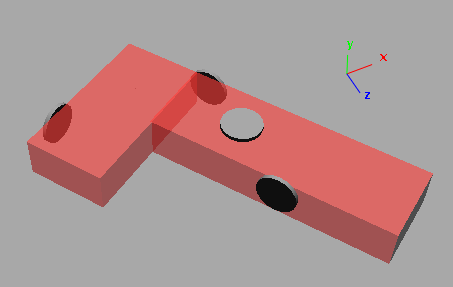
\includegraphics[width=6cm]{img/piece_alone.png}
			\caption{Piece overview. Top connector is for the robots, side connectors are for the other pieces.}
			\label{fig:piece_alone_overview}
		\end{figure}
	
		We created a set of four different pieces, each with different shapes and different connecting capabilities. See Figure~\ref{fig:pieces_types} for the different pieces.
		
		\begin{figure}[h]
			\centering
				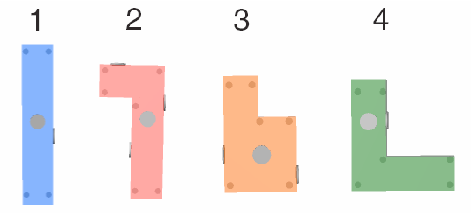
\includegraphics[width=8cm]{img/pieces_types.pdf}
			\caption{Four different pieces created, with their different connecting capabilities.}
			\label{fig:pieces_types}
		\end{figure}
		
		These pieces are endowed with several other capabilities:
		\begin{enumerate}
			\item They have a radio emitter/receiver to communicate with robots or other pieces. The communication range is set to 40cm for the pieces.
			\item They can activate or deactivate their connectors at will.
			\item They know what type they are and where are their connectors.
			\item They know the assembly plans to create the different final puzzles. They also know how they should be oriented for optimal assembly with a give other piece. We will see later that this can be relaxed.
			\item They are fairly intelligent, meaning that they have computational capabilities. The pieces can communicate with other robots, maintain a internal state of their situation.
		\end{enumerate}
		
		\subsubsection{Assembly plans} % (fold)
		\label{ssub:assembly_plans}
			We consider two final puzzles in our project. There are several way of assembling them. We first study two specific plans, but will generalize that when trying to control the chemical reactions network. The two plans and the different mid-assemblies resulting are presented in Figure~\ref{fig:assembly_plans}.
			
			\begin{figure}[h!]
				\centering
				\subfigure[First final puzzle plan] 
				{
					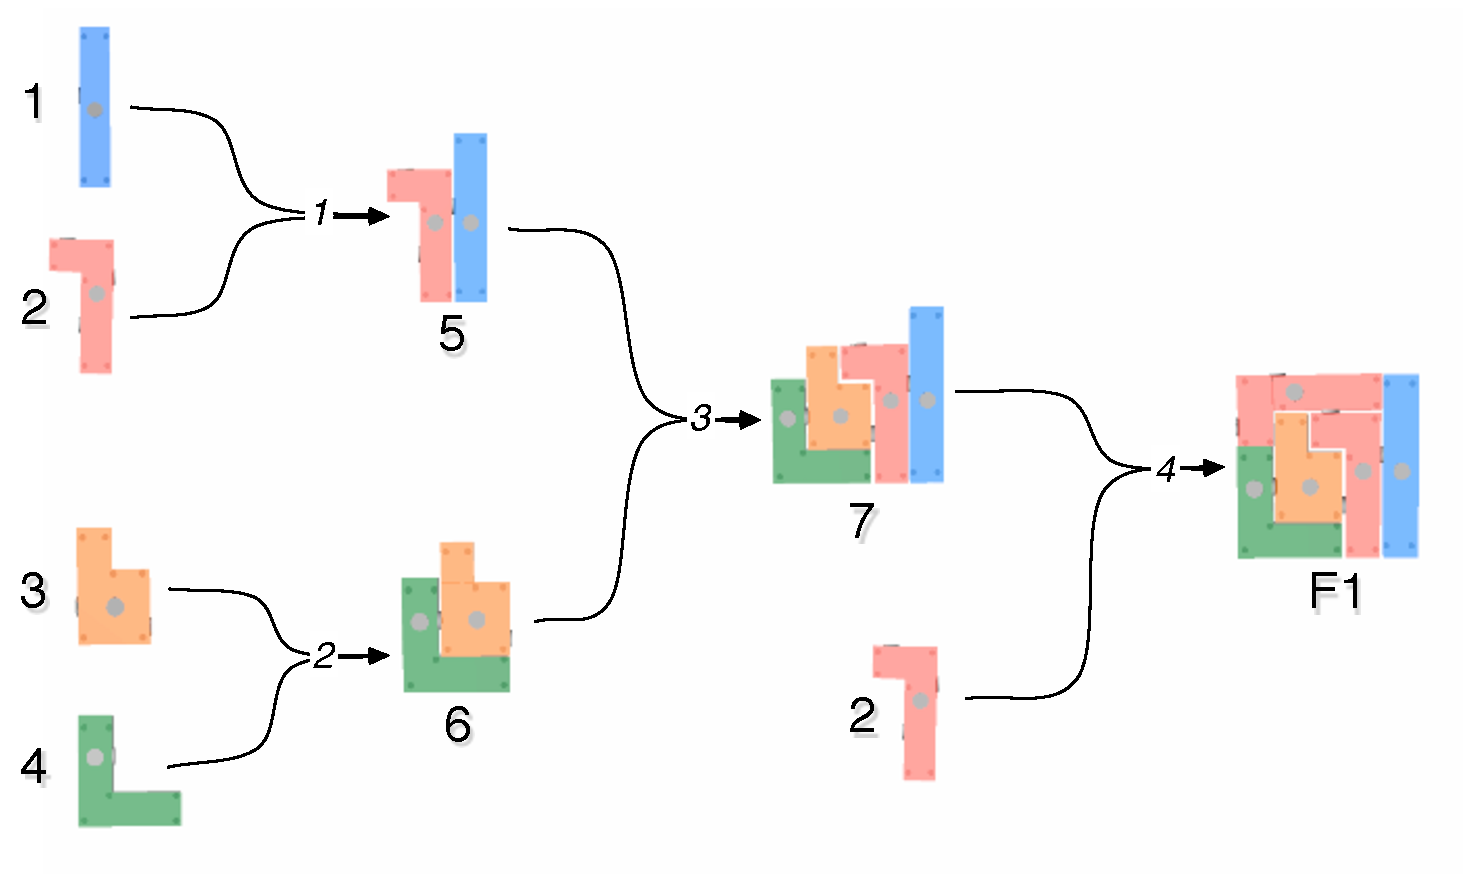
\includegraphics[width=11cm]{img/assembly_plan_f1.pdf}
					\label{fig:assembly_plans:f1}
			 	}
				\; % espacement entre figures. \quad \;
				\subfigure[Second final puzzle plan] 
				{
					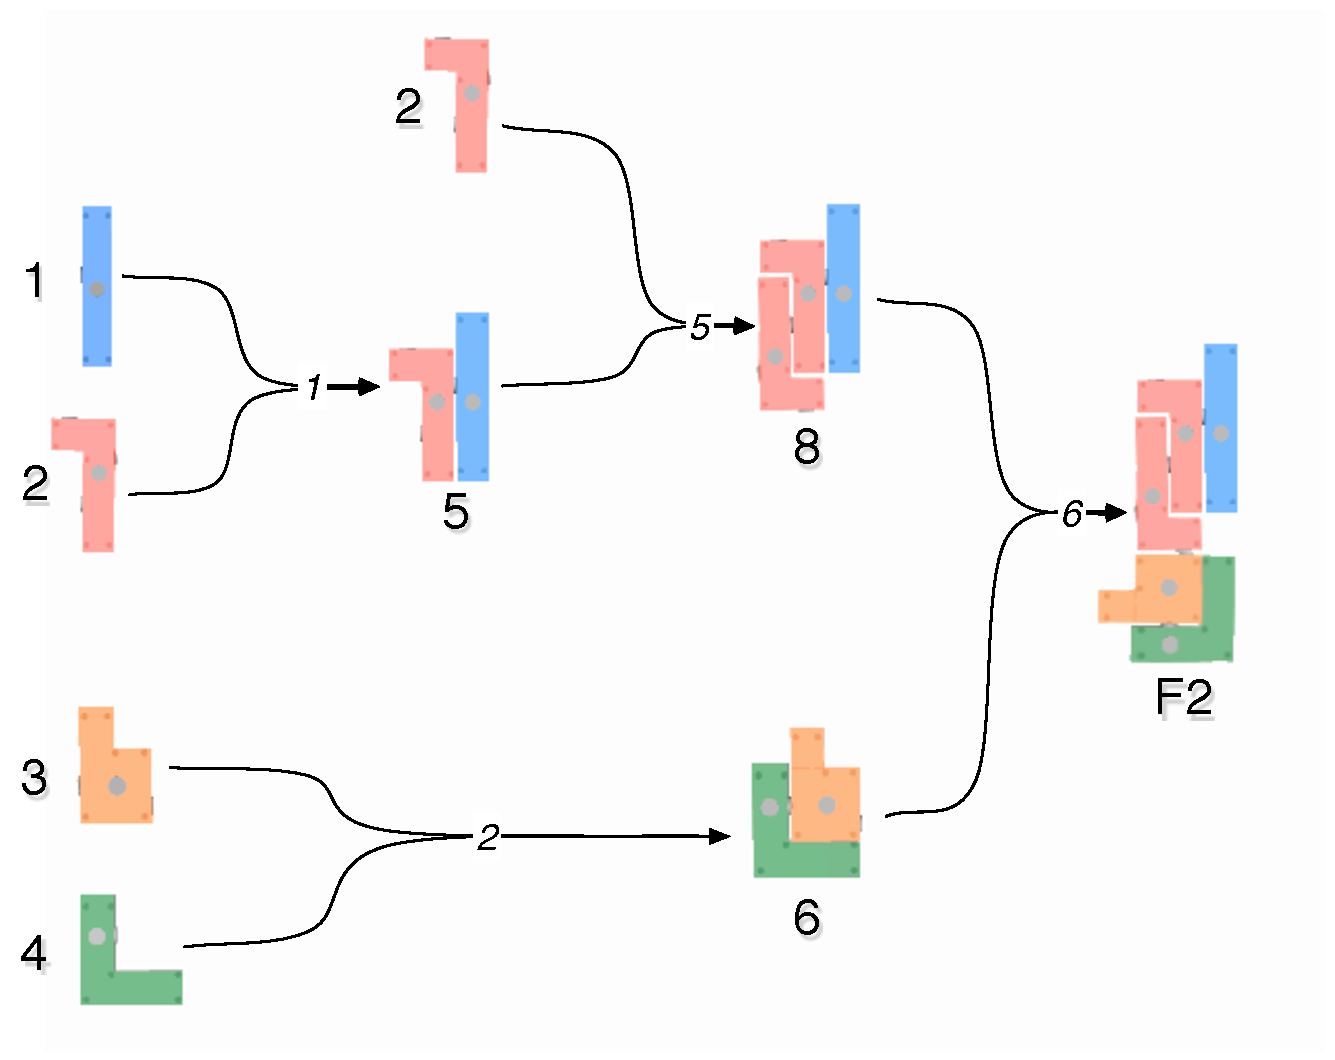
\includegraphics[width=11cm]{img/assembly_plan_f2.pdf}
					\label{fig:assembly_plans:f2}
			 	}
				\caption{Assembly plans for the two final puzzles considered. All groups of connected pieces (mid-assemblies or products) are given an unique name in a form of a number. Arrows show the assembly steps, with their name as number.}
			\label{fig:assembly_plans} %Cation general
			\end{figure}

		% subsubsection assembly_plans (end)
			
	% subsection pieces (end)
	
	\subsection{Robots} % (fold)
	\label{sub:robots}
	For the robots, we used the KheperaIII model available in Webots. It offered a small scale yet not too crude mobile robot for our first implementation.
	
	In order to manipulate the pieces, we equipped the robots with a protruding carrying arm (see Figure~\ref{fig:robot_overview}). This arm consists of a simple bar with a mobile Connector at its end. The Connector is allowed to turn around 360$^{\circ}$ using a rotational Servo, in order to orient the carried piece in any possible direction. The length of the arm is sufficient to rotate any mid-assembly without hitting the robot's body.

	\begin{figure}[h!]
		\centering
		\subfigure[KheperaIII robot.] 
		{
			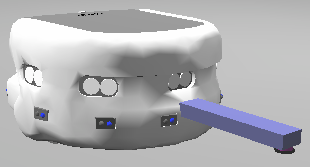
\includegraphics[height=3cm]{img/robot_overview_all.pdf}
			\label{fig:robot_overview_all}
	 	}
		\; % espacement entre figures. \quad \;
		\subfigure[Protruding arm, with rotating connector.] 
		{
			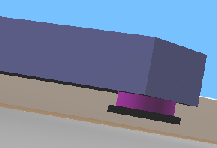
\includegraphics[height=3cm]{img/robot_overview_arm.pdf}
			\label{fig:robot_overview_arm}
	 	}
		\caption{KheperaIII robot model in Webots, with protruding arm.}
	\label{fig:robot_overview} %Cation general
	\end{figure}
	

	When being carried, the piece does not touch the ground, as they are very light-weight.
	
	The robots have similar components to the pieces:
	\begin{my_itemize}
		\item They have a radio emitter/receiver, to communicate with pieces and other robots. The communication range is set to 60cm for the robots. This local radio is also used as a bearing detection mechanism, giving the relative angle between two emitter/receivers. This is used when a robot needs to grab a piece, or when the piece has to be rotated by the rotating arm of a given angle.
		\item They can control the rotation of the servo at the tip of their protruding arm.
		\item They communicate with their carried piece to know what type it is and what is its relative angle.
		\item They know the assembly plans to create the final puzzles.
		\item They move around randomly in the arena, while avoiding other robots and walls using their infra-red distance sensors.
	\end{my_itemize}
	
	\subsubsection{Movement pattern} % (fold)
	\label{ssub:movement_pattern}
	We want our robots to be evenly distributed around the arena in average. This property, the \textit{well-mixed} property, allows us to use non-spatial mathematical models.
	
	\begin{figure}[h!]
		\centering
		\subfigure[Covered space, 3D] 
		{
			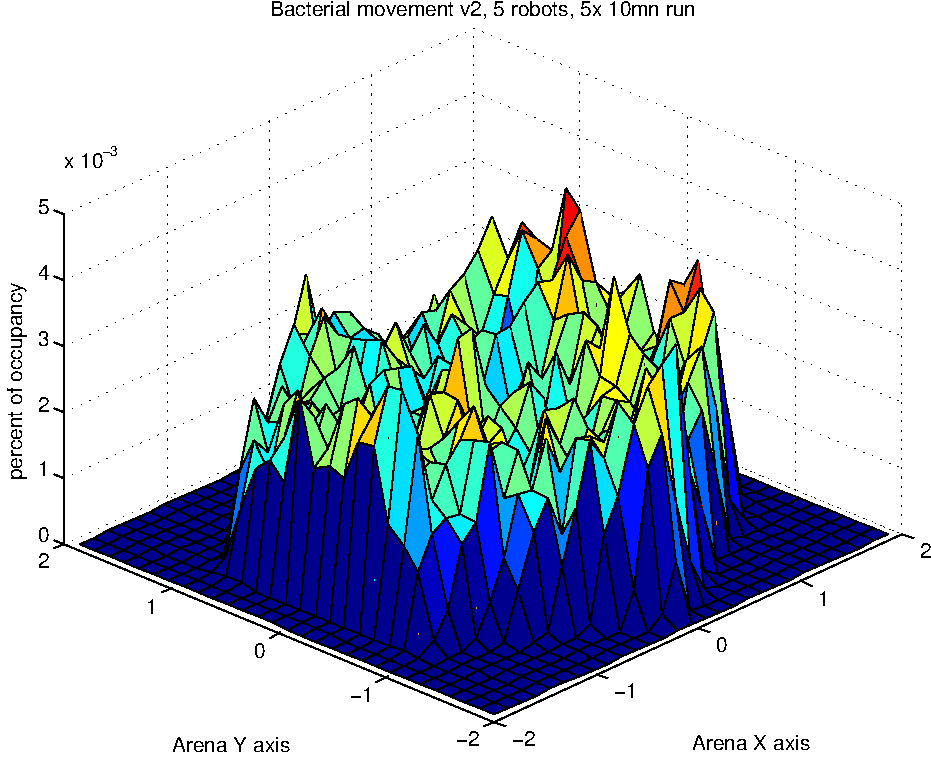
\includegraphics[width=6.5cm]{img/bacterial_covering_3d.pdf}
			\label{fig:img_bacterial_covering_3d}
	 	}
		\; % espacement entre figures. \quad \;
		\subfigure[Covered space, 2D] 
		{
			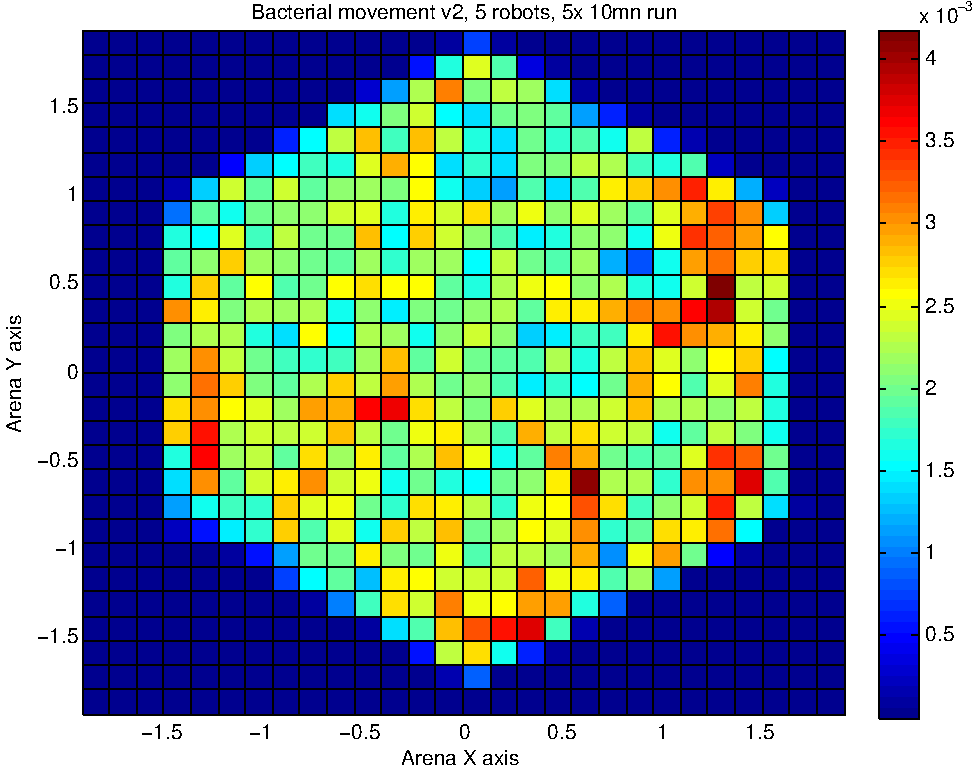
\includegraphics[width=6.5cm]{img/bacterial_covering_2d.pdf}
			\label{fig:img_bacterial_covering_2d}
	 	}
		\caption{Average coverage of the arena by 5 robots moving in a brownian-like motion, over 5 runs of 10 minutes.}
	\label{fig:covering_brownian} %Cation general
	\end{figure}
	
	In order to satisfy this property, the robots have to move around in a specific manner. We chose to make them move in a bacterial-like movement. This movement, ``chemotaxis'', allows bacteria to move around, search for nutriments and avoid dangers. It is based on a forward movement, and random ``tumbling''. A ``tumble'' is a random turn. The bacteria sample the concentration of nutriments or dangerous chemicals, and performs a temporal integration on them while moving. An increase in a nutriments concentration tends to reduce the number of tumbling, promoting movement towards the spacial gradient. When the gradient is constant, the bacteria performs tumbling at a constant rate~\cite{Berg:2000p10058, Adler:1975p7745, Macnab:1972p7813, Dhariwal:1926p7464}.

	In our case, we do not follow any gradient. We only make the robots move forward for a random distance, and then turn randomly around, before moving forward again. This creates a random movement that is supposed to cover more uniformly the space.
	
	We verified this assumption using Webots and our robots. See Figure~\ref{fig:covering_brownian} for the average space covered by five robots over 5 runs of 10 minutes each. We see that the space is nearly evenly covered, which shows that our property is ensured.
	
	
	% subsubsection movement_pattern (end)
	
	\subsubsection{Behavior} % (fold)
	\label{ssub:behavior}
		The robots and the pieces are placed randomly in an hexagonal arena of fixed size. They can only communicate in a local range: 40cm for robot to piece, 60cm for robot to robot. The behavior is then as follows:
		
		\begin{figure}[h]
			\centering
			\; % espacement entre figures. \quad \;
			\subfigure[Encountering between a robot and a piece. The robot aligns itself with the piece.] 
			{
				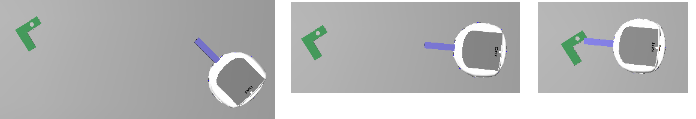
\includegraphics[width=10cm]{img/align_approach_piece.png}
				\label{fig:img_align_approach_piece}
		 	}
			\; % espacement entre figures. \quad \;
			\subfigure[Alignment of piece by the rotating connector] 
			{
				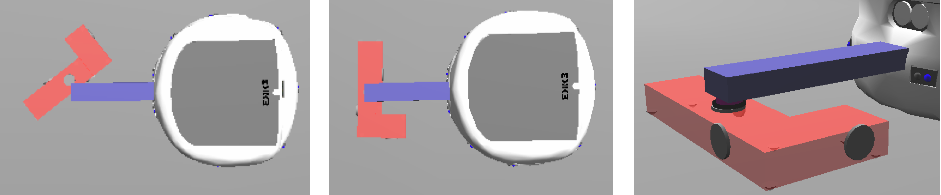
\includegraphics[width=10cm]{img/rotate_piece.png}
				\label{fig:img_rotate_piece}
		 	}
			\; % espacement entre figures. \quad \;
			\subfigure[Approach between two robots and assembling of pieces.] 
			{
				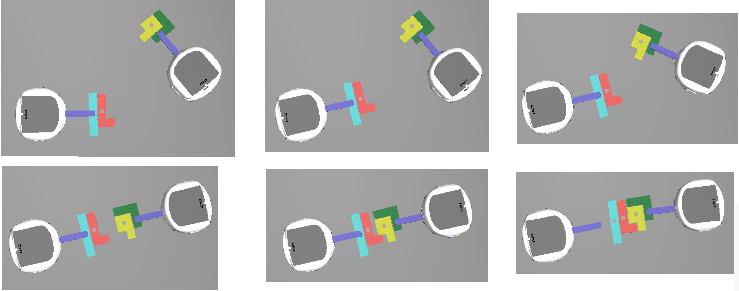
\includegraphics[width=10cm]{img/align_approach.png}
				\label{fig:img_align_approach}
		 	}
			\caption{Assembly behavior of robots and pieces.}
		\label{fig:behavior_webots_assembly} %Cation general
		\end{figure}
		
		
		\begin{my_itemize}
			\item Robots move around, searching for lying pieces. They avoid the walls and other robots using a Braitenberg vehicle controller. The move around randomly following the bacterial-like movement pattern presented before.
			\item Robots and pieces broadcast messages locally, telling their current configuration and state. A configuration is a unique name for a set of assembled pieces, for all possible assemblies present in the plans we are using to build the final puzzles.
			\item When a robot receives a message from a free piece (i.e. they are in a small communication range), it aligns with it, go towards it and carries it. This alignment uses relative range and bearing offered by the emitter/receiver nodes of Webots. See Figure~\ref{fig:img_align_approach_piece}.
			\item While carrying the piece, the robot start moving around again, searching for another robot with a compatible piece. Robots communicate with small range messages broadcasted at all time.
			\item When two robots carrying pieces come into communication ranges, they exchange message and look into the assembly plan. If their pieces correspond to no stored assembly step, they moves away from each other. 
			\item If their pieces can be assembled, the robot start an assembly procedure. According to the piece type and the assembly plan, the robot first orient their pieces so as to show the good connector in front. Again we use the relative range and bearing of emitter/receiver nodes to perform that alignment. This step will be relaxed in a experimental scenario to account for a random orientation of pieces for the assembly. See Figure~\ref{fig:img_rotate_piece}.
			\item Then the robot align each other. The robot starts to approach, allowing the pieces to lock to each other. When the two pieces are locked, one of the robot leaves, letting the other one with the assembled pieces. This robot resume searching for a new piece to assemble with, while the newly freed robot starts looking for a lying piece. See Figure~\ref{fig:img_align_approach}
		\end{my_itemize}
		
	% subsubsection behavior (end)
	
	% subsection robots (end)
	
	\subsection{Experiment platform} % (fold)
	\label{sub:experiment_platform}
	
		Our goal is to reproduce experiments extensively and study the data in Matlab. We thus need a pretty robust system, as well as a centralized way to prepare and store these experiments.
		
		The robustness is ensured by adding several checks and reset capabilities in the behaviors of the robots and pieces. There are still problems that could arise, for example due to physical simulation problems, or a discrepancy between the actual state of the simulation and the way the robots see it. We can only measure what the robots know, so this can create some problems.
		
		As a centralized medium for the experiments, we use a supervisor node in Webots. This supervisor takes care of the experiments and writes the results to different files. It resets the experiments after a maximum elapsed time and takes care of the initial random positions of all pieces and robots. When an assembly step occurs, robots send specific messages to that supervisor, which will save them accordingly.
		
	% subsection experiment_platform (end)
	
	\subsection{Python world generator} % (fold)
	\label{sub:python_world_generator}
		
		Webots does not provide an easy way of varying the components of a given world. However, as we want to control easily the number of robots, pieces, the size of the arena and several other parameters. Therefore, we created our own Webots world generator, in Python.
		
		This world generator is available online on the mailing group of Webots, as it was build to be easily extended. It takes the following inputs:
		
		\begin{my_itemize}
			\item A set of template files. They store parts of a classical Webots VRML world file, but with added free parameters in them.
			\item A input XML file describing the world to create. This file defines which templates to use and how many instances of them to create and finally assigns values to the free parameters.
		\end{my_itemize}
		
		It is easy to add new templates and extend this to different applications.
		
		This generator allows us to generate experimental worlds containing different numbers of pieces and robots easily. We study for now a world with 5 pieces and 4 or 5 robots, and a world with 15 pieces and 15 robots.
		
	% subsection python_world_generator (end)
% section webots_implementation (end)

\section{The robot transporters scenario} % (fold)
\label{sec:the_robot_transporters_scenario}

\paragraph{Characteristics:} % (fold)
\label{par:characteristics_}
Lying pieces, robots carry and assemble them.
% paragraph characteristics_ (end)

This system represents either a self-assembly task if we abstract the robots, or a transporting and assembly task. The pieces can not move and rely on the robots to create a puzzle.

\subsection{Simulation results} % (fold)
\subsubsection{Experiment 1: 5 pieces and 4 robots, final puzzle F1 only} % (fold)
\label{ssub:experiment_1_5_pieces_and_4_robots}

Setup:
\begin{my_itemize}
	\item Hexagonal arena, radius 2m.
	\item 100 experiments.
	\item 20 minutes maximum per experiment.
	\item Pieces and robots initialized at random positions.
	\item Pieces are aligned by the robots before an assembly.
	\item Robots follow the plan to create the final puzzle F1 only, given in Figure~\ref{fig:assembly_plans:f1}.
\end{my_itemize}


\begin{figure}[h!]
	\centering
	% \hspace{-30pt}
	\subfigure[Averaged populations of products over time.] 
	{
		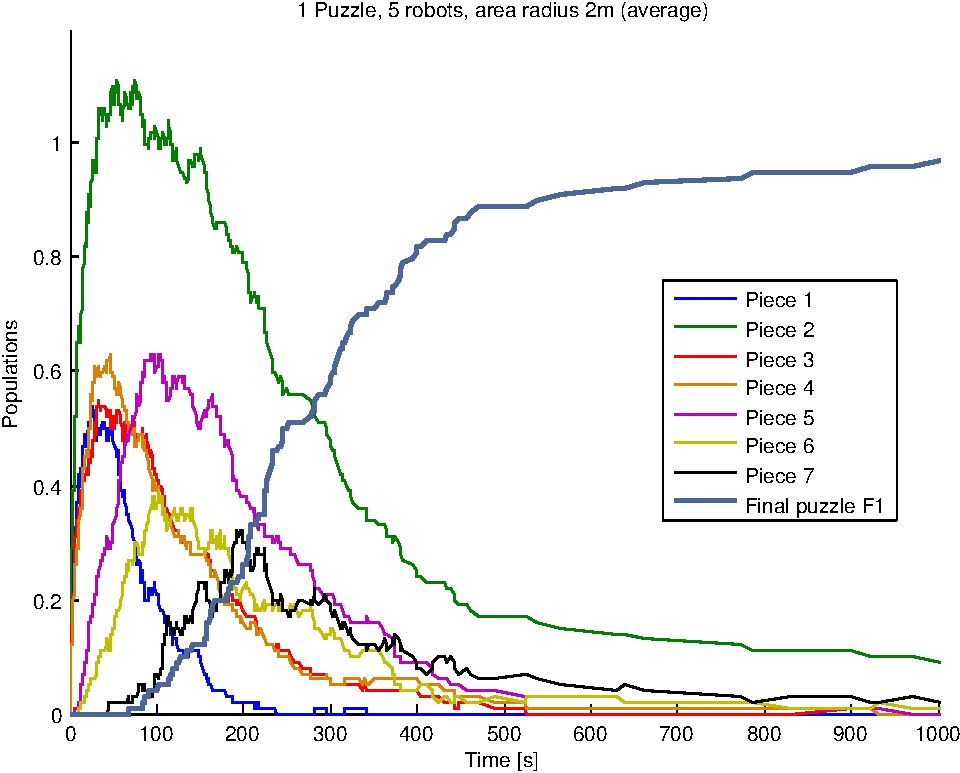
\includegraphics[width=9cm]{img/webots_measure_1puzzle_alone.pdf}
		\label{fig:transporters_experiment1:timeseries}
 	}
	% \; % espacement entre figures. \quad \;
	\subfigure[Histogram of the finishing times of the final puzzles F1. Red line at 400 seconds shows the 75\% quantile.] 
	{
		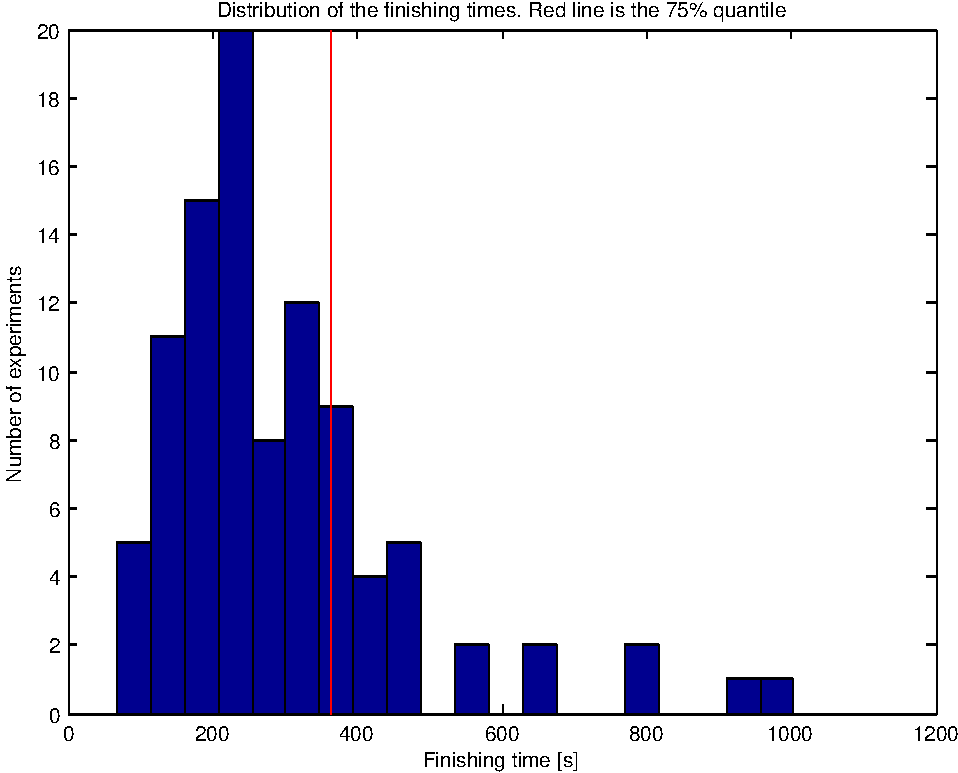
\includegraphics[width=9cm]{img/webots_measure_1puzzle_finishingtimes.pdf}
		\label{fig:transporters_experiment1:finishingtimes}
 	}
	\caption{Physical simulation results for the robot transporter scenario, Experiment 1: 5 pieces, 4 robots and final puzzle F1 only.}
\label{fig:transporters_experiment1} %Cation general
\end{figure}

We see on Figure~\ref{fig:transporters_experiment1:timeseries} that the final puzzle F1 follows an exponential saturating curve, tending toward 1. This is what we expected, as only one puzzle can be created. The curve does not attain exactly 1, meaning that some assemblies are not successful. Indeed, we have a success rate of assembly after 20 minutes of 96\%.

But looking at Figure~\ref{fig:transporters_experiment1:finishingtimes}, which shows the histogram of the times of creation of the final puzzles over all experiments, we see that 75\% of the puzzles are actually completed after 6 minutes and 40 seconds on average. This is a good results, as it means that most of the experiments were completed quickly.

% subsubsection experiment_1_5_pieces_and_4_robots (end)

\subsubsection{Experiment 2: 15 pieces and 15 robots, final puzzle F1 only} % (fold)
\label{ssub:experiment_2_15_pieces_and_15_robots_final_puzzle_f1_only}

Setup:
\begin{my_itemize}
	\item Hexagonal arena, radius 3m.
	\item 100 experiments.
	\item 20 minutes maximum per experiment.
	\item Pieces and robots initialized at random positions.
	\item Pieces are aligned by the robots before an assembly.
	\item Robots follow the plan to create the final puzzle F1 only, given in Figure~\ref{fig:assembly_plans:f1}.
\end{my_itemize}

\begin{figure}[h!]
	\centering
	\subfigure[Averaged populations of products over time.] 
	{
		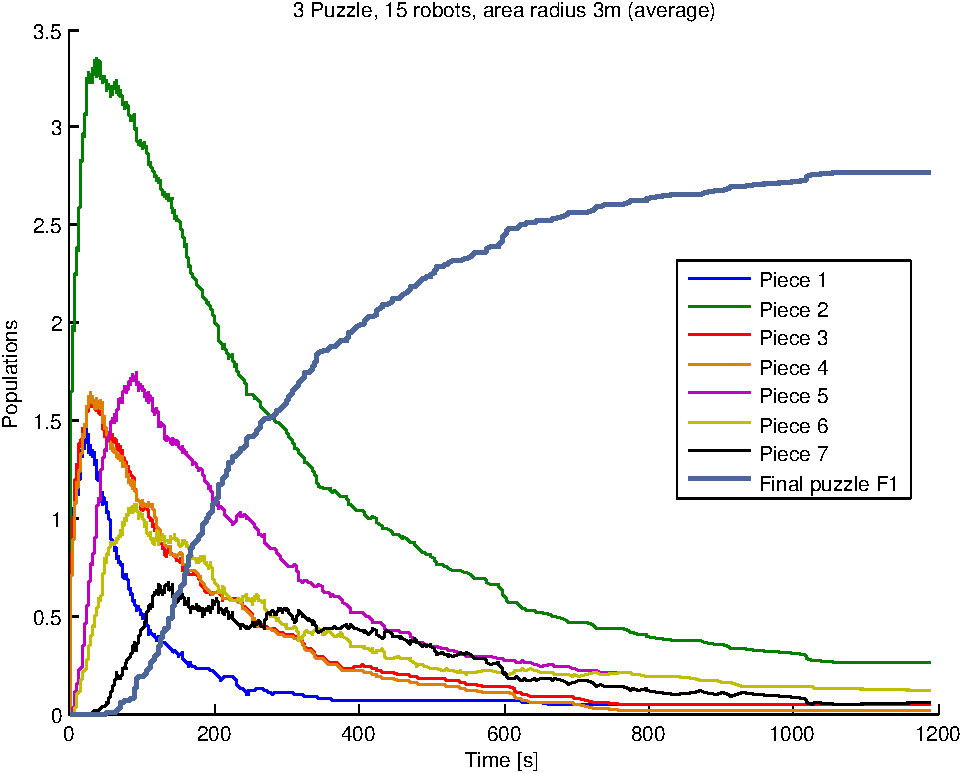
\includegraphics[width=9cm]{img/webots_measure_3puzzle_alone.pdf}
		\label{fig:transporters_experiment2:timeseries}
 	}
	\; % espacement entre figures. \quad \;
	\subfigure[Histogram of the finishing times of the final puzzles F1. Red line at 400 seconds shows the 75\% quantile.] 
	{
		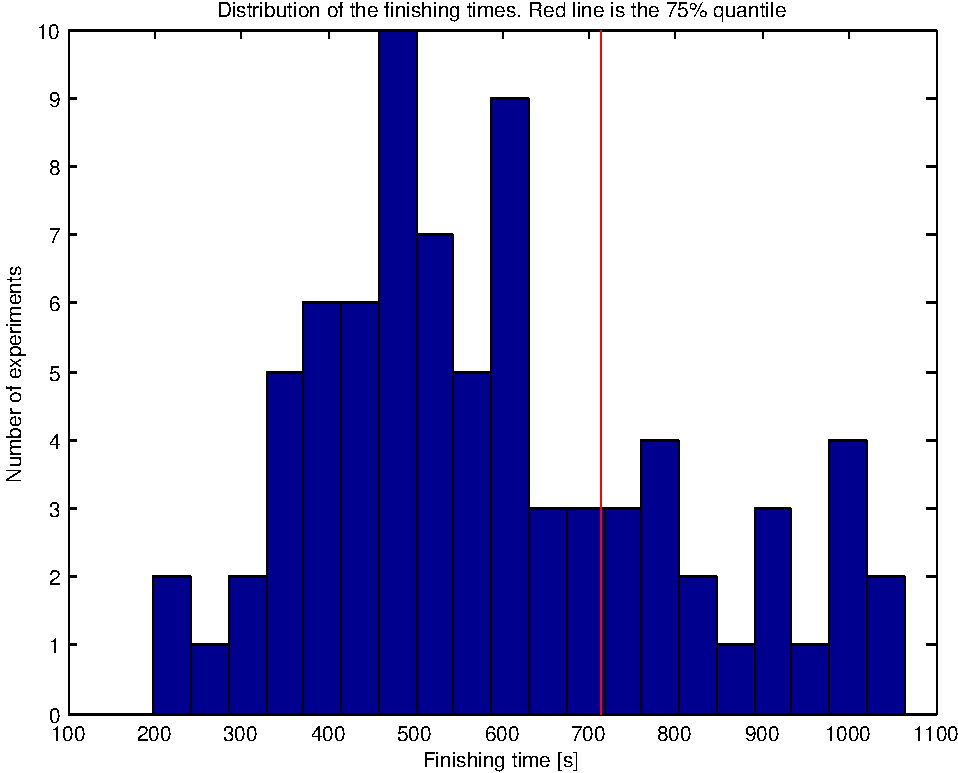
\includegraphics[width=9cm]{img/webots_measure_3puzzle_finishingtimes.pdf}
		\label{fig:transporters_experiment2:finishingtimes}
 	}
	\caption{Physical simulation results for the robot transporter scenario, Experiment 2: 15 pieces, 15 robots and final puzzle F1 only.}
\label{fig:transporters_experiment2} %Cation general
\end{figure}

Figure~\ref{fig:transporters_experiment2:timeseries} shows a similar behavior than before. The curve is smoother, due to the bigger amount of pieces and possible final puzzles. The curve again tends exponentially towards the maximal puzzle number, 3. But it converges to an even smaller number, as more assemblies goes wrong. After 20 minutes, we have a success rate of assembly of 3 puzzles of 80\% only. This shows that some things can still go wrong in our physical simulations, which affects the final assembly yield.

Looking at Figure~\ref{fig:transporters_experiment2:finishingtimes}, we see that the 75\% quantile for the successfully assembled 3 final puzzles is at 11 minutes. This is still a pretty good result, which shows that our approach is scalable to a higher number of pieces and robots, assuming that the space available for the movements does not become too small.

% subsubsection experiment_2_15_pieces_and_15_robots_final_puzzle_f1_only (end)

\subsubsection{Experiment 3: 5 pieces and 5 robots, final puzzles F1 and F2} % (fold)
\label{ssub:experiment_3_5_pieces_and_5_robots_final_puzzles_f1_and_f2}

Setup:
\begin{my_itemize}
	\item Hexagonal arena, radius 2m.
	\item 100 experiments.
	\item 20 minutes maximum per experiment.
	\item Pieces and robots initialized at random positions.
	\item Pieces are aligned by the robots before an assembly.
	\item Robots follow the plans to create the final puzzles F1 and F2. See Figure~\ref{fig:assembly_plans}.
\end{my_itemize}


\begin{figure}[h!]
	\centering
	\subfigure[Averaged populations of products over time.] 
	{
		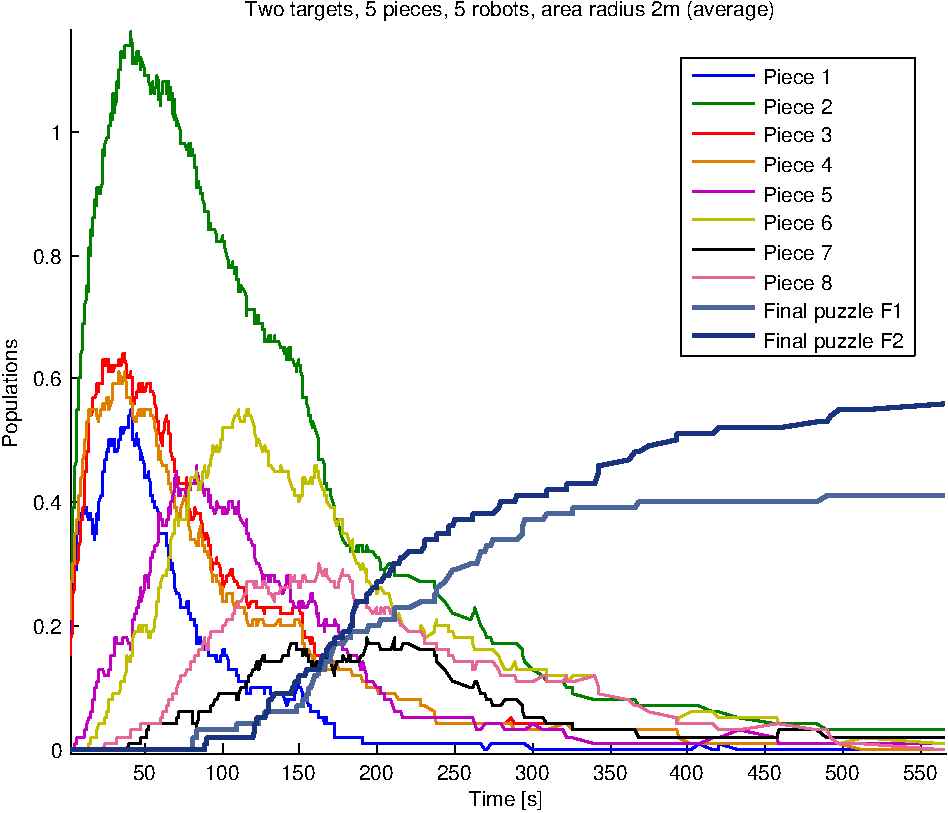
\includegraphics[width=9cm]{img/webots_measure_twotargets_1puzzle_alone.pdf}
		\label{fig:transporters_experiment3:timeseries}
 	}
	\; % espacement entre figures. \quad \;
	\subfigure[Histogram of the finishing times of either final puzzle F1 or F2. Red line at 400 seconds shows the 75\% quantile.] 
	{
		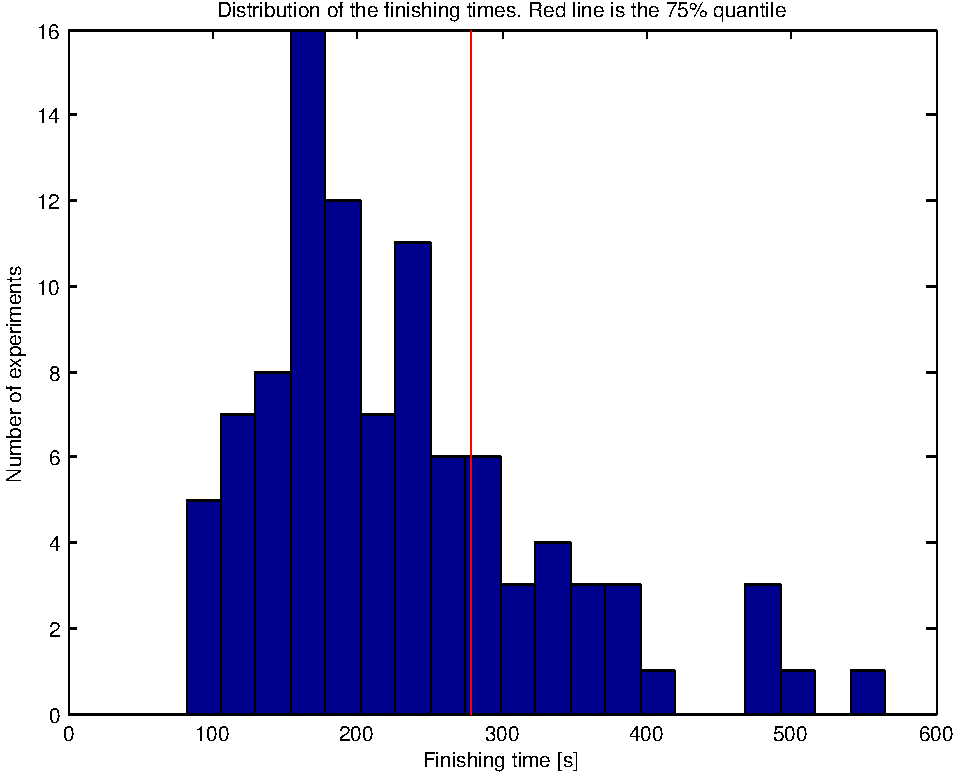
\includegraphics[width=9cm]{img/webots_measure_twotargets_1puzzle_finishingtimes.pdf}
		\label{fig:transporters_experiment3:finishingtimes}
 	}
	\caption{Physical simulation results for the robot transporter scenario, Experiment 3: 5 pieces, 5 robots and final puzzles F1 and F2.}
\label{fig:transporters_experiment3} %Cation general
\end{figure}

Figure~\ref{fig:transporters_experiment3:timeseries} shows an interesting result. We see that the two final puzzle converge to a value that sum (more or less) to $1$. But the distribution between the two assemblies is not even, we have $60\%$ of final puzzle $F2$ and $40\%$ of final puzzle $F1$. By looking at the assembly plans and the available initial pieces, we think it is due to reaction 5. This reaction uses piece 5, which is created early, and uses another piece 2, which is easily available (purple curve and green curve). Compared to reaction 3, which uses a piece 5 and a piece 6, which takes more time to be produced, there is less time dependence on the path to F2. This tends to promote it.

This discrepancy triggered the idea of being able to control the ratio between the two final puzzles, by modifying the system. This will be the subject of our Augmentation step and optimization of the model, Chapter~\ref{cha:chemical_reaction_networks_control_and_design} and \ref{cha:augmented_assembly_implementation}.

From Figure~\ref{fig:transporters_experiment3:finishingtimes}, we see that the 75\% quantile for the successfully assembled final puzzle is at 4 minutes 30 seconds, with a success ratio of $97\%$. This is again very good, few assemblies go bad, even with the two possible final puzzles.
% This is better than for experiment 1, which can be explained by the added robot. 

% subsubsection experiment_3_5_pieces_and_5_robots_final_puzzles_f1_and_f2 (end)

% \subsubsection{Experiment 4: random alignment of pieces before assemblies} % (fold)
% \label{ssub:experiment_4_random_alignment_of_pieces_before_assemblies}
% 
% Setup:
% \begin{my_itemize}
% 	\item Hexagonal arena, radius 2m.
% 	\item 100 experiments.
% 	\item 20 minutes maximum per experiment.
% 	\item Pieces and robots initialized at random positions.
% 	\item Carried pieces are rotated randomly when moving around.
% 	\item The pieces are not aligned before an assembly.
% 	\item Robots follow the plans to create the final puzzles F1 and F2. See Figure~\ref{fig:assembly_plans}.
% \end{my_itemize}
% 
% % subsubsection experiment_4_random_alignment_of_pieces_before_assemblies (end)

% subsection simulation_results (end)
% section the_robot_transporters_scenario (end)

\section{The self-assembling pieces scenario} % (fold)
\label{sec:the_self_assembling_pieces_scenario}
When the pieces can move around and assemble on their own, robots are not necessary anymore. This scenario is closer to a real nano self-assembly task, but at a macro-scale level.

We developed such a scenario in Webots, using the same pieces with several modifications:
\begin{my_itemize}
	\item The pieces are pushed by individual forces, of randomly chosen direction. The pieces have a low friction coefficient with the floor to allow easy movement.
	\item There are forces applied onto the pieces when they approach the walls too closely. This introduce a wall-avoidance in a smooth fashion. The repulsive force $F_r$ applied is directed toward the center of the arena and an amplitude inversely proportional to the current distance to the walls:
	\[
		F_r \sim \frac{1}{\left(\sqrt{x^2+y^2} - R_a sin(\frac{\pi}{3}) \right)^2} \cdot \left( 
		\begin{array}{c} -x \\
			-y \end{array} \right)
	\]
	$R_a sin(\frac{\pi}{3})$ is the radius of the incircle to the hexagonal arena of radius $R_a$. 
	\item The pieces attracts each others in a small radius. This was introduced to improve the encountering rate, which was not comparable to the one we had before. Indeed, a collision of two pieces is less likely than the encountering of two communication circles as we had before. This force attracts the pieces for some time, and then repulse then, to mimic a missed assembly.
\end{my_itemize}

All these modifications create a scenario where the assembly rates are much smaller than before, but which can still create some final puzzles. Unfortunately, due to robustness issues, we did not manage to get systematic experiments in time for that scenario. Its study will be done in further works.

% section the_self_assembling_pieces_scenario (end)

\section{The mixed assembly scenario} % (fold)
\label{sec:the_mixed_assembly_scenario}

We can combine the two last scenarios into this fully complex one. The pieces can move around and assemble on their own, but can also be carried around and assembled by robots.

In order to make the carrying possible, the pieces stop moving when a robot is trying to grab them. Moreover, a free piece cannot interact with a carried piece. The robot has to drop it first.

This scenario closely resembles a biological process with enzymatic components. The pieces assemble following their own dynamics, which are improved by the robots via their specific actions and orientation capabilities.

Again we did not manage to completely study this scenario. We leave it as further work, not without regrets.
% chapter puzzle_test_case_implementation (end)

\chapter{Mathematical model of the puzzle test-case} % (fold)
\label{cha:mathematical_model_of_the_puzzle_test_case}
	
\section{Model definition} % (fold)
\label{sec:model_definition}
	We introduce now the mathematical model used to represent our puzzle test-case system. As told earlier, we use a chemical reaction network framework (see Section~\ref{sec:chemical_reaction_networks} for background on this subject).

	We only consider the robot transporters scenario, the other scenario can be modeled in the same fashion.
	
	We assign a reaction to each assembly step in the creation of the final puzzles. Looking back at Figure~\ref{fig:assembly_plans}, each numbered assembly step corresponds to a reaction in our chemical reaction network.
	Furthermore, we add 4 new reactions, representing the grabbing of lying pieces by the robots.
	The products and reactants are the different mid-assemblies, plus the 3 lying free pieces and the robots. All reactions are second-order reactions, as they depend on the encountering of two different reactants upon reaction.
	
	We obtain the following chemical reaction network (Equation~\eqref{eq:reaction_network_transportersimple}):
	
	\begin{eqnarray}
		X_R + X_1^f ~~\xrightarrow{e_1} ~~ X_1 & \quad  & X_R + X_3^f ~~\xrightarrow{e_3} ~~ X_3 \nonumber \\
		X_R + X_2^f ~~\xrightarrow{e_2} ~~ X_2 & & X_R + X_4^f ~~\xrightarrow{e_4} ~~ X_4 \nonumber \\
		X_1 + X_2 ~~\xrightarrow{k_1} ~~ X_5 + X_R &  &  X_2 + X_7 ~~ \xrightarrow{k_4} ~~ X_{F1} + X_R\nonumber \\
		X_3 + X_4 ~~\xrightarrow{k_2} ~~ X_6 + X_R& & X_2 + X_5	~~ \xrightarrow{k_5} ~~ X_{8} + X_R \nonumber \\
		X_5 + X_6 ~~\xrightarrow{k_3} ~~ X_7 + X_R & & X_6 + X_8 ~~ \xrightarrow{k_6} ~~ X_{F2} + X_R
	\label{eq:reaction_network_transportersimple}
	\end{eqnarray}
	
	$X_R$ is a robot, $X_i^f$ are the free lying pieces, $X_k$ are the carried pieces and $X_{Fj}$ the final puzzles.
	
	The variables can be defined as the number of each piece type, where the number is a continuous function of time~\cite{Gillespie:1977p5555}. This network can then be transformed in the following associated ODE system (Equation~\eqref{eq:ode_transportersimple}):
	
	\begin{equation}
		\left\lbrace\begin{array}{lll}
			\dot{x_R} & = & -\sum_{l=1}^4 e_lx_Rx_l^f + k_1x_1x_2 + k_2x_3x_4 +  \\
			& & \qquad k_3x_5x_6 + k_4 x_2 x_7 + k_5 x_2 x_5 + k_6 x_6 x_8 \\
			\dot{x_1^f} & = & -e_1x_Rx_1^f \\
			\dot{x_2^f} & = & -e_2x_Rx_2^f \\
			\dot{x_3^f} & = & -e_3x_Rx_3^f \\
			\dot{x_4^f} & = & -e_4x_Rx_4^f \\
			\dot{x_1} & = & e_1x_Rx_1^f -k_1x_1x_2 \\
			\dot{x_2} & = & e_2x_Rx_2^f -k_1x_1x_2 -k_4x_2x_7 -k_5x_2x_5\\
			\dot{x_3} & = & e_3x_Rx_3^f -k_2x_3x_4 \\
			\dot{x_4} & = & e_4x_Rx_4^f -k_2x_3x_4 \\
			\dot{x_5} & = & k_1x_1x_2 -k_3x_5x_6 - k_5x_2x_5  \\
			\dot{x_6} & = & k_2x_3x_4 -k_3x_5x_6 - k_6x_6x_8 \\
			\dot{x_7} & = & k_3 x_5 x_6 -k_4 x_2 x_7 \\
			\dot{x_8} & = & k_5 x_2 x_5 -k_6x_6x_8 \\
			\dot{x}_{F1} & = & k_4x_2x_7 \\
			\dot{x}_{F2} & = & k_6x_6x_8 
		\end{array}\right.
		\label{eq:ode_transportersimple}
	\end{equation}
	
	Obviously, this notation is less compact, yet has the same meaning.
	
	We can also represent the network in matrix form:
	
	\[
		\mathbf{\dot{x}} = \mathbf{S} \mathbf{K} \mathbf{y}
	\]
	$\mathbf{S}$ is the stoichiometric matrix, containing the stoichiometric coefficients $m_r$ and $n_p$ as defined in Equation~\eqref{eq:general_chemical_reaction} in Section~\ref{sub:theory}. $\mathbf{K}$ is the matrix of stochastic constant rates. $y$ is a vector of compounds, in our case the set of all bilinear terms in Equation~\eqref{eq:ode_transportersimple} for example.
	
	We can also relax the $x_R$ and $x_i^f$ terms, if we decide to look only at the real assembly process therein. Doing so is consistent if we assume that we have a big number of robots to carry the pieces around, and that they grab the pieces very quickly compared to the actual assembly process. This approach is similar as doing a quasi-steady state simplification, for a multiscale system where the robots are acting quicker than the rest of the system. Such a relaxation simplifies the whole system and its analysis, we will use it in the next chapter.
% section model_definition (end)

	\subsection{Simulation of the model} % (fold)
	\label{sub:simulation_of_the_model}
		We simulate our models using two different approaches:
		\begin{enumerate}
			\item ODE solving. We use Matlab to solve numerically the system \eqref{eq:ode_transportersimple}, using a classical ode45. We use libSBML~\cite{Bornstein:2008p7529} for Matlab to write and read from SBML files onto ODE files.
			\item Stochastic Simulation Algorithm. We use the StochKit toolbox~\cite{Li:2008p11431}, developed by Petzold et al. StochKit is a simulation framework for stochastic simulations written in C++. It allows a very fast exact simulations of chemical reaction networks.
		\end{enumerate}
	% subsection simulation_of_the_model (end)
	
\section{Parameter fitting} % (fold)
\label{sec:parameter_fitting}
	
	\subsection{Theoretical value of reaction rates} % (fold)
	\label{sub:theoretical_value_of_reaction_rates}
	
		The chemical reaction network is easy constructed from the assembly plans considered, but we still need to find values for the stochastic constant rates~$k_i$ and~$e_l$.
	
		We decompose the stochastic constant rates as follows:
	
		\begin{equation}\label{eq:reaction_assembly_rate}
			k_i = p^e_i \cdot p^a_i
		\end{equation}
	
		where $p^e_i$ is the probability of an encounter between two elements and $p_i^a$ the probability of successful assembly.
	
		$p_i^a$ can be easily measured, or assumed to be $1$ if the robots manage to align the pieces correctly before each assembly step.
	
		If we assume that our model is non-spatial, i.e. that the probability that two product are at a given position is independent of the time and uniformly distributed over the available arena space, we can make an initial informed guess on the encountering probability. We take an approach used in~\cite{Correll:2007p8184, Correll:2007p8236, Correll:2006p8328}, giving the following relation for the encountering probability:
	
		\begin{equation} \label{eq:encountering_probability}
			p^e_i \sim \frac{1}{A_{total}}v_rTw_d^i
		\end{equation} 
	
		Where $A_{total}$ is the arena size, $v_r$ is the average speed of an element, $T$ is the timestep (fixed to $1$ in our case) and $w_d^i$ the width of detection of an element. This expression can actually be linked back to the literature on chemical process simulations~\cite{Gillespie:1992p8126, Puchalka:2004p4312, Turner:2004p4446}. For chemical process, the probability of collision depends on the volume swept by one molecule, which gives the probability that another molecule will collide it in the next $dt$. Equation~\eqref{eq:encountering_probability} is exactly the same, as shown on Figure~\ref{fig:volume_swept}. In our case, as we work in a 2D plan, we only have surface swept, which is exactly given by the right part of \eqref{eq:encountering_probability}. Dividing by the total arena size and assuming the elements are distributed uniformly in the arena, this gives directly the probability of encountering between two elements.
	
		\begin{figure}[h]
			\centering
			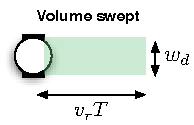
\includegraphics[width=4cm]{img/volume_swept.pdf}
			\caption{Graphical interpretation of the encountering probability and link to the volume swept used in chemical simulations.}
			\label{fig:volume_swept}
		\end{figure}
	
		In our test case, we measured $v_r$ over 50 simulation runs using the robot movement pattern described earlier, the average speed was $0.128 m/s$. $A_{total}$ is also easily computed ($=6 (R^2\frac{\sqrt{3}}{4})$, i.e. the sum of the six equilateral triangles of radius $R$). $w_d^i$ becomes the double of the communication radius between robots or pieces, as it defines the range for the start of an assembly.
	
	% subsection theoretical_value_of_reaction_rates (end)
	
	\subsubsection{Rates verification} % (fold)
	\label{ssub:rates_verification}
		We checked this initial guess by measuring the encountering rates in Webots. We create a world with one lying piece and one searching robot, we measure the time to encounter, over 200 experiments. As discussed in the theory of chemical reaction networks, these times are distributed following an exponential of the encountering probability. We load the times in Matlab, and fit an exponential distribution to get this probability (Figure~\ref{fig:img_encountering_exp_fitting}).
		\begin{figure}[h]
			\centering
				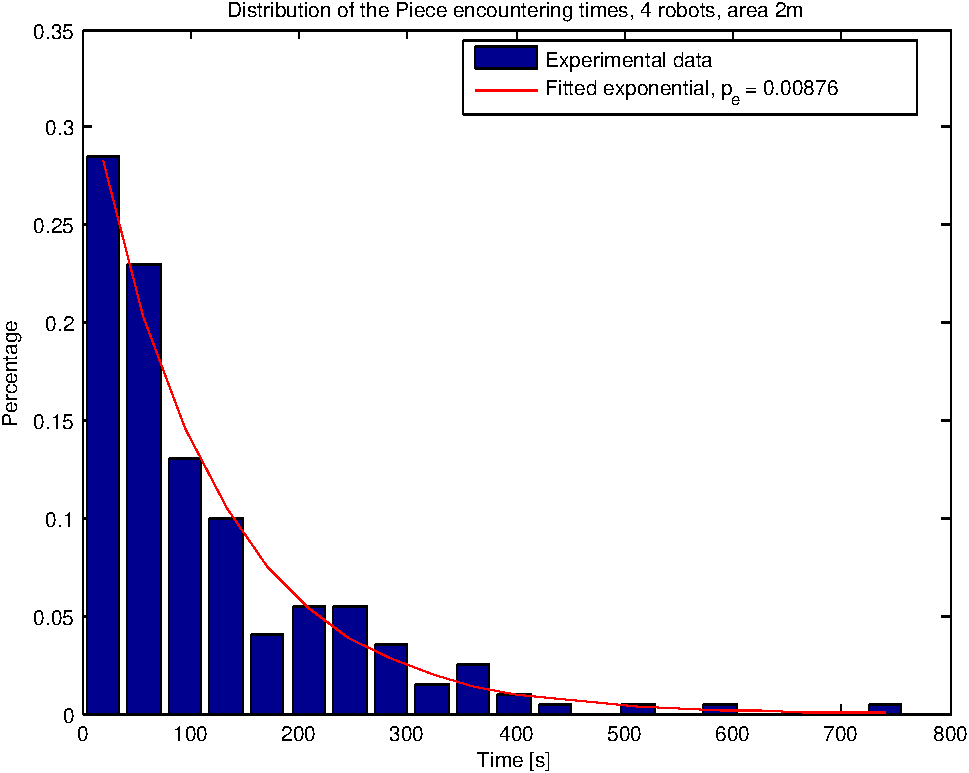
\includegraphics[width=9cm]{img/encountering_exp_fitting.pdf}
			\caption{Encountering times for the Webots experiment, with the fitted Matlab exponential.}
			\label{fig:img_encountering_exp_fitting}
		\end{figure}
		
		We also add ``dummy'' robots in the arena, that only avoid each other without looking for the piece. It measures the effect of overcrowding on the well-mixed property we're trying to ensure within our Webots simulation.
		
		\begin{figure}[h]
			\centering
				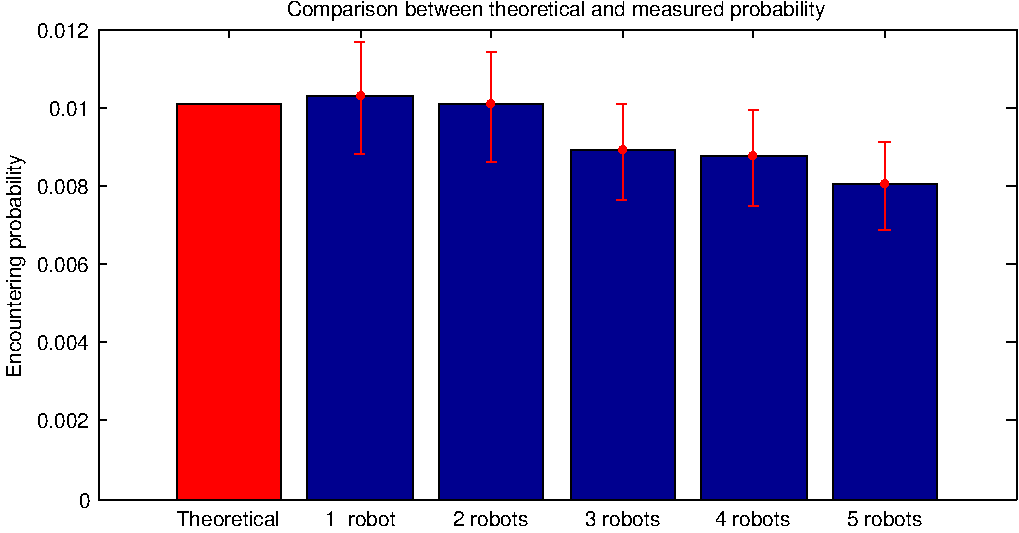
\includegraphics[width=11cm]{img/encounteringrate_withrobots.pdf}
			\caption{Comparison between the theoretical guess for the encountering probability $p_e^i$ and the measured encountering probability in Webots. The red intervals represents the confidence intervals for the fitted encountering probability.}
			\label{fig:img_encounteringrate_withrobots}
		\end{figure}
		
		The results of the comparison between the theoretical and measured rates of encountering are shown in Figure~\ref{fig:img_encounteringrate_withrobots}. We see that the theoretical guess is pretty accurate, even tough it is overestimated when more robots are present. The added robots seems to disturb the capacity of a robot to encounter a piece. This can be due to the fact that the robots perturbs the trajectories while avoiding each others, overcrowding some areas and forbidding the access to others.
		
		The same measurement was performed for robot to robot encountering and gave similar results. We do not show it here.
		
	% subsubsection rates_verification (end)	
% section parameter_fitting (end)

\section{Comparison with physical simulation} % (fold)
\label{sec:comparison_with_physical_simulation}
	
	We simulate the chemical reaction network \eqref{eq:reaction_network_transportersimple} using the two approaches presented in Section~\ref{sub:simulation_of_the_model}. Depending on the initial conditions for the number of robots and pieces, we have different experiments, following Section~\ref{sec:the_robot_transporters_scenario}.
	
	\subsubsection{Stochastic constant rates values} % (fold)
	\label{ssub:stochastic_constant_rates_values}
		Through all these experiments, the stochastic constant rates $e_l$ and $k_i$ take similar values, conditioned by specific parameters presented in each experiment setup.
		
		\begin{description}
			\item[Encountering rates] $e_l = \frac{1}{A_{total}}\cdot v_r \cdot w_d^p \quad \forall l \in \{1..4\}$.
			\item[Reaction rates] $k_i = p^a_i\cdot \frac{1}{A_{total}}\cdot v_r \cdot w_d^r \quad \forall i$.
			\item[Arena size] $A_{total}=3 \cdot R_a^2 \cdot \frac{\sqrt{3}}{2}$.
			\item[Average speed] $v_r = 0.128$ measured in Webots.
			\item[Piece communication width] $w_d^p = 2\cdot0.4m$, pieces are set to communicate in a $40cm$ radius.
			\item[Robot communication width] $w_d^r = 2\cdot0.6m$, robots are set to communicate in a $60cm$ radius.
			\item[Probability of successful assembly] $p^a_i$ depends on the experiment being studied, more precisely on the assembly plan used. We measured it in Webots, over 100 runs, for the assembly plan creating only the final puzzle F1 and for the assembly plan creating the final puzzles F1 and F2. Results will be specified in the experiments' setup.
		\end{description}
	
	% subsubsection stochastic_constant_rates_values (end)
	
	\subsection{Experiment 1: 5 pieces and 5 robots, final puzzle F1 only} % (fold)
	\label{sub:experiment_1_5_pieces_and_5_robots_final_puzzle_f1_only}
		Setup:
		\begin{description}
			\item[Initial conditions:] $X_R = 5, X_1^f=1, X_2^f=2, X_3^f=1, X_4^f=1, X_i=0, X_{Fk}=0$.
			\item[Experiment duration:] 20 minutes.
			\item[Number of experiments (Stochastic simulation only):] 100.
			\item[Arena size:] $R_a = 2m$.
			\item[Probability of successful assembly:] all $p^a_i$ where more or less equal to $0.98$. Thus we set $p^a_i = 0.98$.
		\end{description}
				
		See Figure~\ref{fig:models_comparison_experiment1} for the comparison between the simulated chemical reaction networks and the Webots physical simulation. The results from the Webots simulation are taken from Section~\ref{ssub:experiment_1_5_pieces_and_4_robots}. We show the averaged populations over 20 minutes.
				
		\begin{figure}[h!]
			%\centering
			\subfigure[ODE simulation vs physical Webots simulation] 
			{
				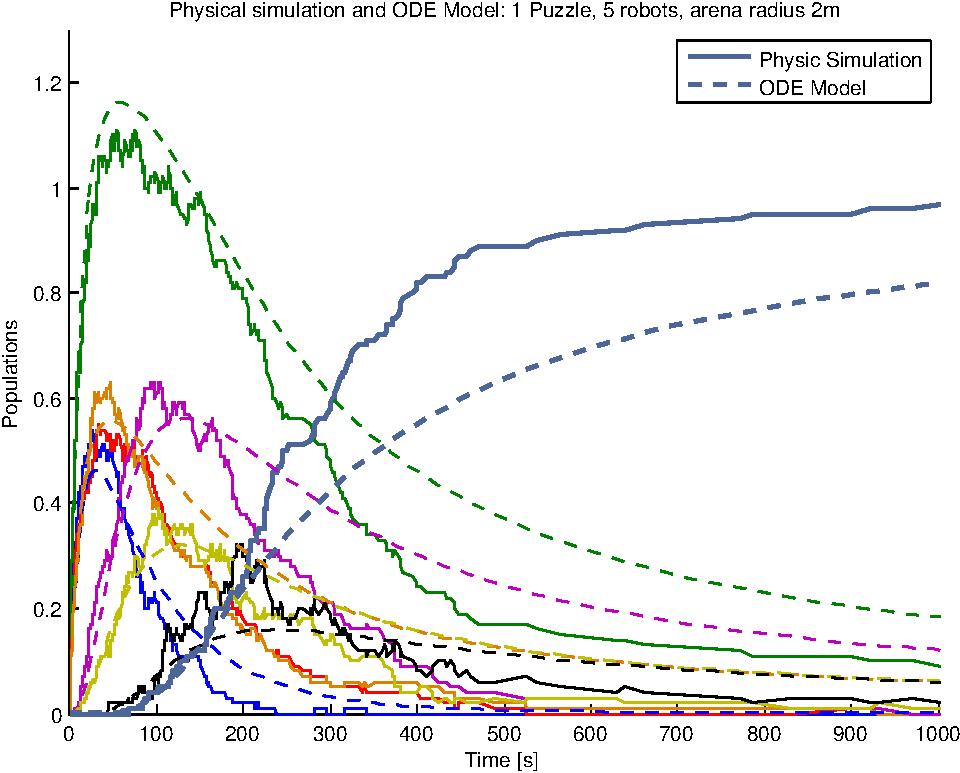
\includegraphics[width=7cm]{img/odereal_1puzzle.pdf}
				\label{fig:models_comparison_experiment1:odereal}
		 	}
			\: % espacement entre figures. \quad \;
			\subfigure[Stochastic simulation vs physical Webots simulation] 
			{
				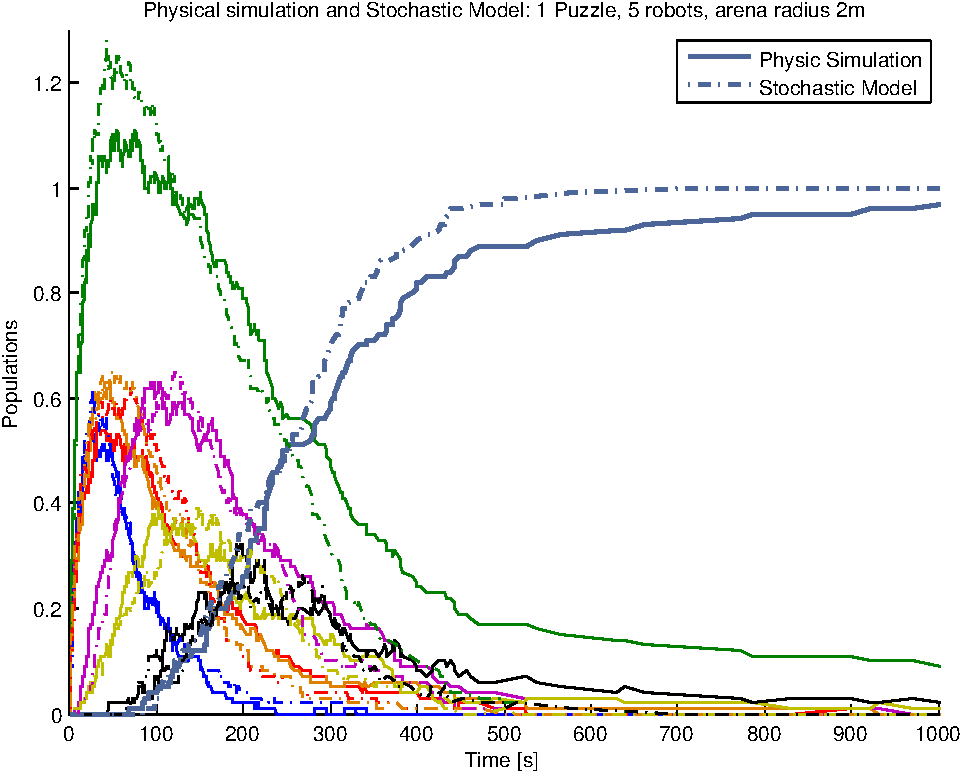
\includegraphics[width=7cm]{img/stochreal_1puzzle.pdf}
				\label{fig:models_comparison_experiment1:stochreal}
		 	}
			\caption{Comparison between the models simulations and the physical Webots simulation for the puzzle test-case, scenario 1, experiment 1.}
		\label{fig:models_comparison_experiment1} %Caption general
		\end{figure}
			
		We see that they fit closely to the physical simulation. Two differences arise:
		
		\begin{my_itemize}
			\item The ODE simulation population values are too small, because of the slow copy number of components (Figure~\ref{fig:models_comparison_experiment1:odereal}). When doing an ODE approximation, one assumes that the number of components is big enough so that using continuous numbers does not have much effects. This is not the case here, where we work with numbers smaller than $10$. On the other hand, the Stochastic simulation accurately captures this property, as it works with discrete numbers. 
			\item The stochastic simulation attains 1, whereas the physical simulation stays below (Figure~\ref{fig:models_comparison_experiment1:stochreal}). These results show that, while there are problems in the Webots simulation (pieces stuck together, blocked against the walls), this is not taken into account in the model. We could modify the model by introducing ways of deactivating some pieces to try to fit this difference. But we do not take much interest in that for this current work.
		\end{my_itemize}
		
	% subsection experiment_1_5_pieces_and_5_robots_final_puzzle_f1_only (end)
	
	\subsection{Experiment 2: 15 pieces and 15 robots, final puzzle F1 only} % (fold)
	\label{sub:experiment_2_15_pieces_and_15_robots_final_puzzle_f1_only} 
		Setup:
		\begin{description}
			\item[Initial conditions:] $X_R = 15, X_1^f=3, X_2^f=6, X_3^f=3, X_4^f=3, X_i=0, X_{Fk}=0$.
			\item[Experiment duration:] 20 minutes.
			\item[Number of experiments (Stochastic simulation only):] 100.
			\item[Arena size:] $R_a = 3m$.
			\item[Probability of successful assembly:] $p^a_i = 0.98$.
		\end{description}
			
		Under the same assumptions than for experiment 1, see Figure~\ref{fig:models_comparison_experiment2} for the comparison in this scenario.			
			
		\begin{figure}[h!]
			%\centering
			\subfigure[ODE simulation vs physical Webots simulation] 
			{
				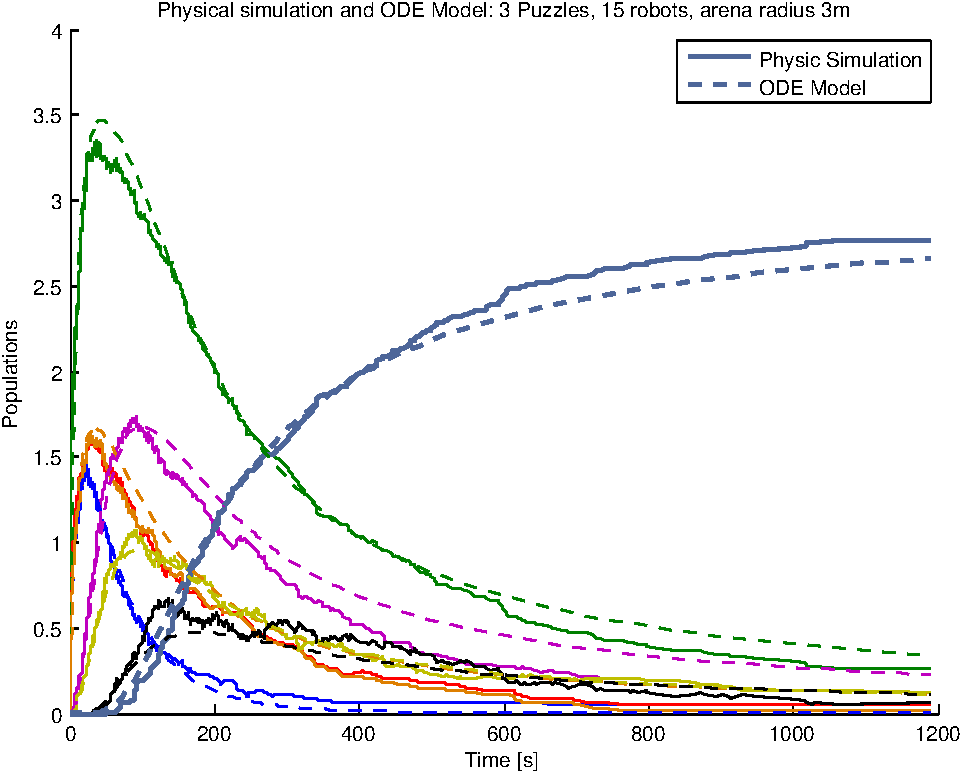
\includegraphics[width=7cm]{img/odereal_3puzzle.pdf}
				\label{fig:models_comparison_experiment2:odereal}
		 	}
			\: % espacement entre figures. \quad \;
			\subfigure[Stochastic simulation vs physical Webots simulation] 
			{
				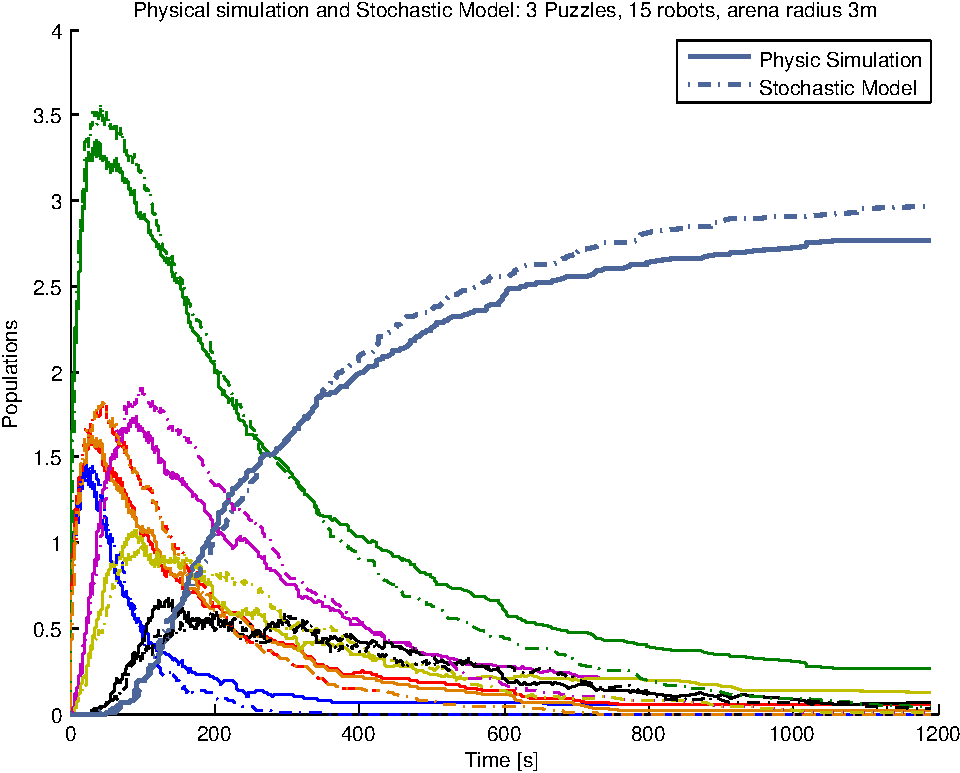
\includegraphics[width=7cm]{img/stochreal_3puzzle.pdf}
				\label{fig:models_comparison_experiment2:stochreal}
		 	}
			\caption{Comparison between the models simulations and the physical Webots simulation for the puzzle test-case, scenario 1, experiment 2.}
		\label{fig:models_comparison_experiment2} %Caption general
		\end{figure}
			
		The results are similar to experiment 1. With a higher number of elements, the ODE simulation is closer to the correct physical simulation. The stochastic simulation is still very accurate but attains the maximal number of puzzles whereas the physical simulation converge to a lower value.
		
	% subsection experiment_2_15_pieces_and_15_robots_final_puzzle_f1_only (end)
	
	\subsection{Experiment 3: 5 pieces and 5 robots, final puzzles F1 and F2} % (fold)
	\label{sub:experiment_3_5_pieces_and_5_robots_final_puzzles_f1_and_f2}
	
		Setup:
		\begin{description}
			\item[Initial conditions:] $X_R = 5, X_1^f=1, X_2^f=2, X_3^f=1, X_4^f=1, X_i=0, X_{Fk}=0$.
			\item[Experiment duration:] 20 minutes.
			\item[Number of experiments (Stochastic simulation only):] 100.
			\item[Arena size:] $R_a = 2m$.
			\item[Probability of successful assembly:] Results of the measures are shown in Table~\ref{tab:assembly_success_experiment3}. We see that now, the probabilities are not equal and depend on the assembly step. Especially, the success of reaction 5, to create piece 8, is significantly smaller. $p^a_i$ is set accordingly for each reaction $i$.
		\end{description}
				
		\begin{table}
			\begin{center}
			\begin{tabular}{|c|c|c|c|c|c|c|}
			 \hline
				\textbf{Reaction} $\mathbf{i}$ & 1 & 2 & 3 & 4 & 5 & 6 \\
			 \hline
				$\mathbf{p^a_i}$ & 0.9777 & 0.9074 & 0.9636 & 0.9737 & 0.833 & 1.0 \\
			 \hline
			\end{tabular}
			\end{center}
			\caption{Probability of successful assembly for experiment 3. Measured over 100 experiments.}
			\label{tab:assembly_success_experiment3}
		\end{table}
		
		See Figure~\ref{fig:models_comparison_experiment3} for the results.
		
		\begin{figure}[h!]
			%\centering
			\subfigure[ODE simulation vs physical Webots simulation] 
			{
				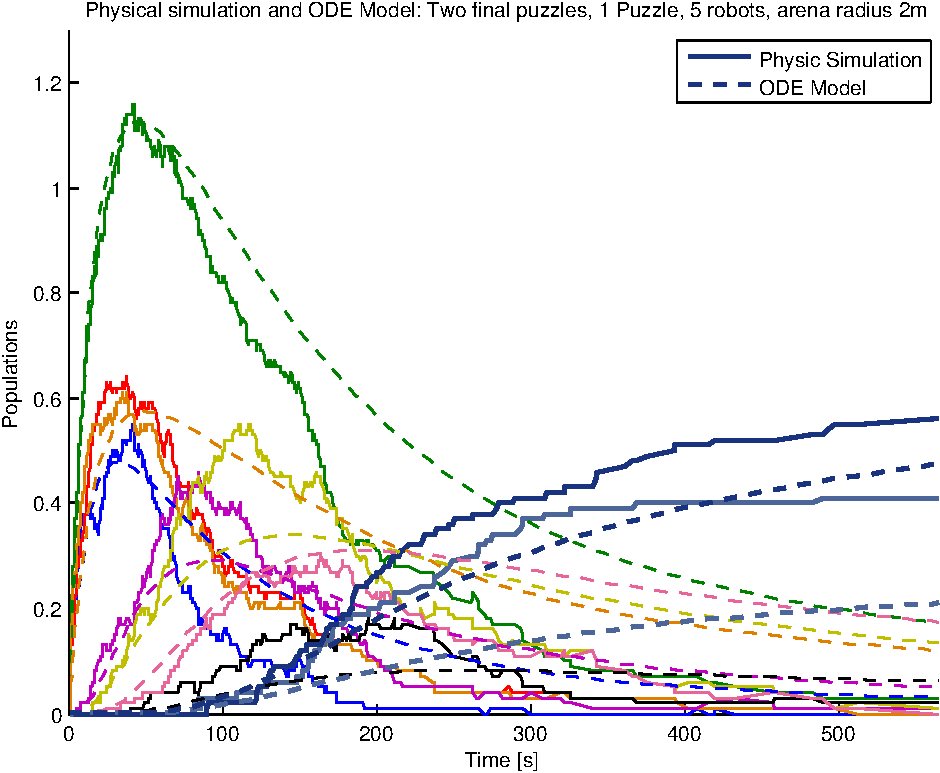
\includegraphics[width=7cm]{img/odereal_2finals_1puzzle.pdf}
				\label{fig:models_comparison_experiment3:odereal}
		 	}
			\: % espacement entre figures. \quad \;
			\subfigure[Stochastic simulation vs physical Webots simulation] 
			{
				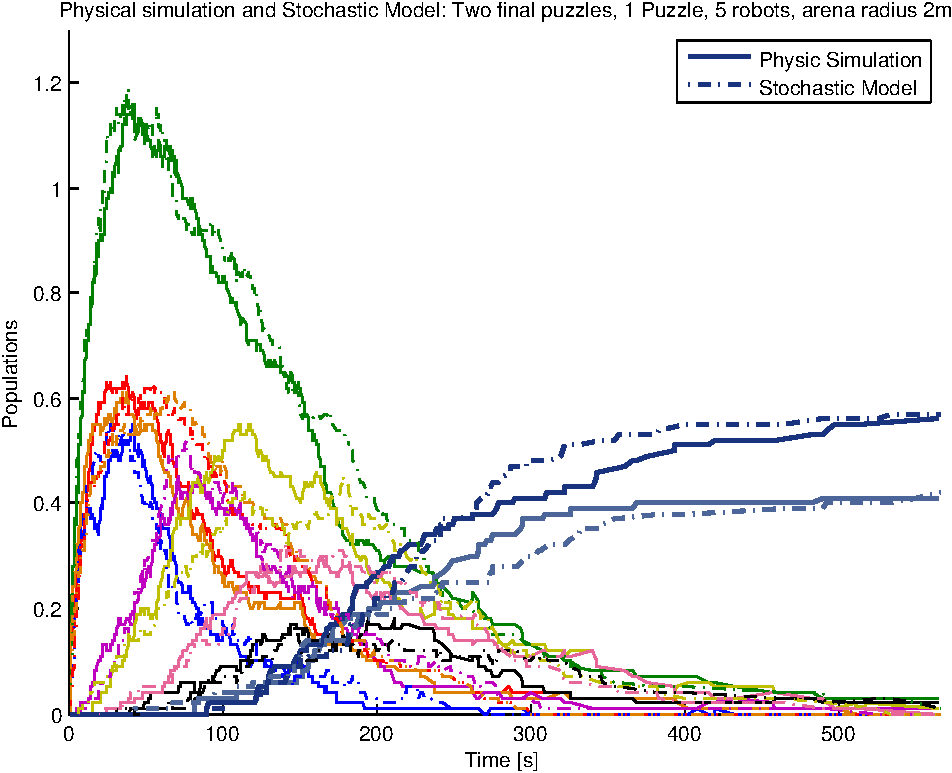
\includegraphics[width=7cm]{img/stochreal_2finals_1puzzle.pdf}
				\label{fig:models_comparison_experiment3:stochreal}
		 	}
			\caption{Comparison between the models simulations and the physical Webots simulation for the puzzle test-case, scenario 1, experiment 3.}
		\label{fig:models_comparison_experiment3} %Caption general
		\end{figure}
		
		We see that the ODE model fails to capture the time to convergence, and underestimates the speed of variations. It also seems that they do not converge to the same values, which could be a problem. However, using the Stochastic simulation with the exact same rates, we see that the fitting is much better. The low copy numbers again has a big impact on the capacity to use the ODE model as an approximation.
			
		But the rates we use for the ODE model produce a good fit when using the Stochastic simulation, which shows that our model accurately describes the physical system's dynamics. We thus think that, if the copy number is big enough, the analysis with the ODE model should be sufficient.
		
		We confirm this hypothesis by performing the same two final puzzles experiment, with 15 pieces and 15 robots and a bigger arena (like Experiment 2). The parameters are adapted accordingly. We obtain the results shown in Figure~\ref{fig:models_comparison_experiment3bis}.
		
		\begin{figure}[h!]
			%\centering
			\subfigure[ODE simulation vs physical Webots simulation] 
			{
				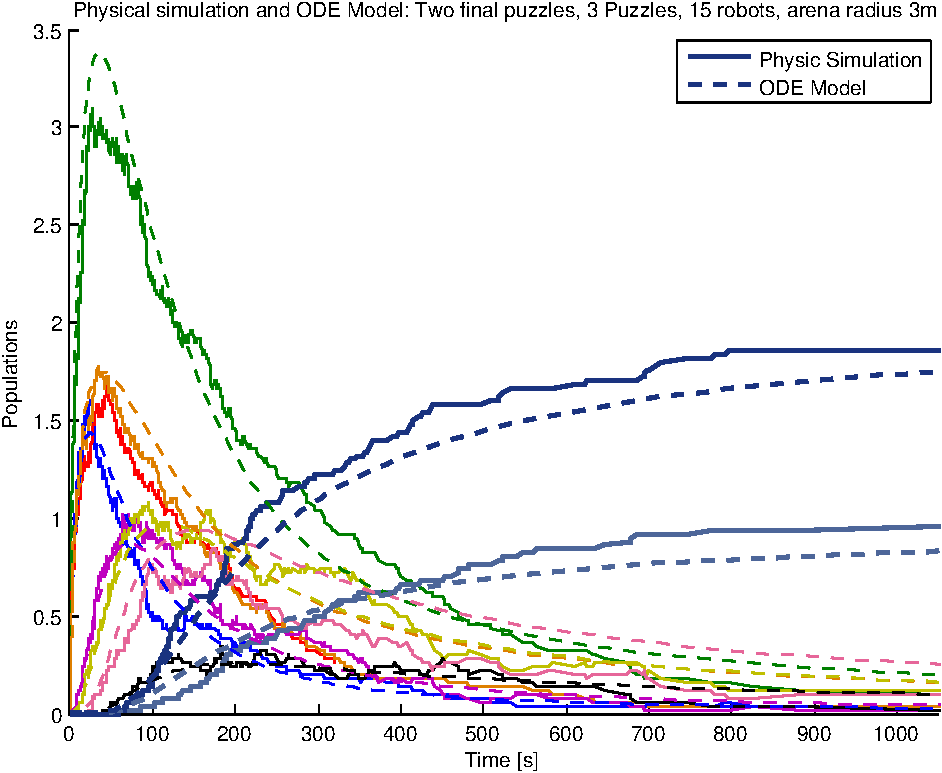
\includegraphics[width=7cm]{img/odereal_2finals_3puzzle.pdf}
				\label{fig:models_comparison_experiment3bis:odereal}
		 	}
			\: % espacement entre figures. \quad \;
			\subfigure[Stochastic simulation vs physical Webots simulation] 
			{
				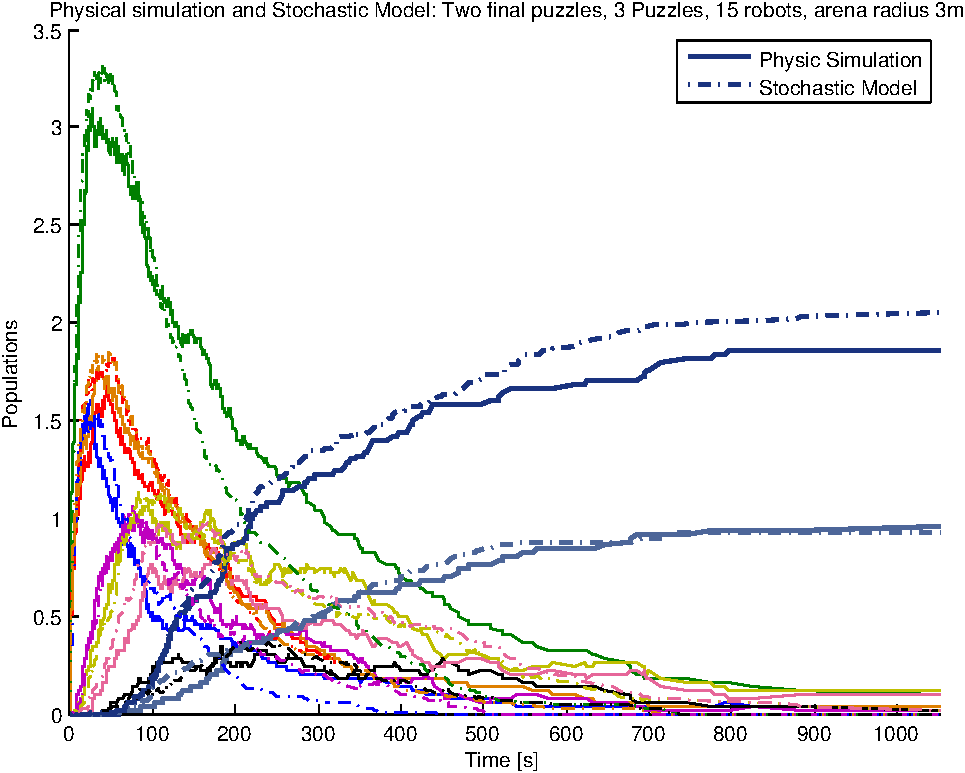
\includegraphics[width=7cm]{img/stochreal_2finals_3puzzle.pdf}
				\label{fig:models_comparison_experiment3bis:stochreal}
		 	}
			\caption{Modified experiment 3 with 15 pieces and 15 robots, to show the effect of a larger copy number.}
		\label{fig:models_comparison_experiment3bis} %Caption general
		\end{figure}
		
		This confirms our assumption that the only problem with the ODE model discrepancy of convergence is the low copy number. In this new scenario, the fitting of the ODE simulation is good and converge to the physical values (Figure~\ref{fig:models_comparison_experiment3bis:odereal}). This tells us that we can indeed use the ODE as a model, but only for a copy number large enough. We will take advantage of that fact in the next chapter.
		
		
	% subsection experiment_3_5_pieces_and_5_robots_final_puzzles_f1_and_f2 (end)
	
% section comparison_with_physical_simulation (end)

\section{Final considerations} % (fold)
\label{sec:final_considerations}
	
	The comparison between the models and the Webots physical simulations shows a close fit of our model to the experimental data. It proves that this model is accurate for our test-case and considered problem. The stochastic simulation captures the correct behavior when the number of elements is small, which is in accordance with the assumptions on algorithms differences.
	
	Therefore, we will use directly the model into an optimization process, before mapping back the new model onto the physical simulation. This approach makes sense, as thanks to the accuracy of our model, we can then hope that the physical simulation will behave in the same way. The only constraint is that we need to work with big copy numbers with the ODE, to avoid convergence problems.
	
	Some problems are still present.
	For example, the initial guess for the encountering probability becomes wrong when the number of robots and pieces grows. The guess relies on a strong non-spatiality constraint, which our physical simulation can not ensure in several cases. Our models do not capture the failures of the physical simulations, which hinder the overall performance and reliability of the assembly process. 
% section final_considerations (end)
% chapter mathematical_model_of_the_puzzle_test_case (end)

% % empty page
\pagebreak
\thispagestyle{empty}
\begin{center}\tiny \sc This page intentionally left blank.\end{center}
\pagebreak


\chapter{Chemical reaction networks control and design} % (fold)
\label{cha:chemical_reaction_networks_control_and_design}
	Having successfully modeled our puzzle test-case using a Chemical Reaction Network, we turn to the next step: modifying this model so that
it behaves in a desired way.

This modification could be making it more efficient (i.e. optimizing it for a given metric) or just attaining a specific goal (i.e. create a specific final distribution). We define the control problem as follows:
\begin{quote}
	Let a system of chemical reactions $R$, defined by a matrix of rate constants $K$, a stoichiometry
matrix $S$ and a vector of products and reactants $y$. Let the initial condition $x_0$ be known also. What should be the matrix $K_c$ so that the system
converges as close as possible to a desired equilibrium $\hat{X}$. Moreover, can we find the matrix $K_{f}$ that converge as close as possible to $\hat{X}$ at
the fastest rate?
\end{quote}

This is a design problem as well as an optimization problem. In the second proposition, we are optimizing for fast convergence subject to a constraint on the equilibrium.

\textit{This part has been done in close collaboration with Spring Berman.}

\section{Overview of possibilities} % (fold) \label{sec:overview_of_possibilities}

	Our first goal was to use a previous optimization scheme used by S. Berman~\cite{ref:BermanTRO08, Halasz:2007p10106}, namely optimizing the Mixing-time of a Markov chain~\cite{Randall:2006p11793, NEthier:1986p4833, Sun:2005p4975}. Unfortunately, our problem is not a Markov chain. Our model is a continuous-time Markov process, with nonlinear rates. Actually, it is possible to represent it as a Markov chain, an approach taken by Klavins for his optimization technique~\cite{Klavins:2007p2600}: we have to consider every possible macro-states or marking of the system starting from an initial condition, by discretizing all possible values taken by the products, and then creating or measuring the probabilities to jump from one macro-state to another. Obviously, this approach runs into a combinatorial explosion when the number of species and their populations increase, which forbids us from using it. Other approaches using Markov chains~\cite{Runolfsson:2007p9740, Tierney:1994p9783} are also abandoned because of this problem.
	
	Therefore, we looked into the chemical reaction networks literature for an optimization scheme taking advantage of the control we have on the stochastic constant rates.
	
	We found papers focusing on the reachability of networks, namely knowing what parts of the state space could be attained knowing the system dynamics~\cite{Berman:2007p10105, Bastin:1993p10351, Kloetzer:2006p9623, Bastin:1990p10531, Batt:2007p9650}. These works apply more to bioreactors and show little interest designing the reaction rates and more on controlling already present reactions.
	Other works, on the other hand, rely too much on a control theory methodology, for example by adding a feedback to the system~\cite{OteroMuras:2008p10653, Iglesias:2007p9153, Belta:2002p12009, Belta:2006p9642}. As we want to modify only the rates, these were not helpful.
	
	Eventually, we found an interesting study in~\cite{Schuster:1987p11838}. The authors propose an analysis and optimization of the rates of a chain of reactions, with respect to several objectives. Those objectives closely resembles the two propositions we are trying to solve, we will therefore use ideas from their work, although our approach is original. However, they are working with reaction chains, which offers simplifications and results that are not available for our more complex reaction network.
	
% section overview_of_possibilities (end)

\section{Methodology} % (fold) \label{sec:methodology}

	\subsection{Changes on our models} % (fold)
	\label{sub:changes_on_our_models}

		Starting from the chemical reaction network \eqref{eq:reaction_network_transportersimple}, we make several modifications in order to satisfy our methodology:
		
		\begin{my_enumerate}
			\item We remove the robots from the system. We assume that the number of robots is bigger or equal to the number of pieces and that the robots find and carry the piece very quickly with respect to the time between assemblies. Under those assumptions, we can remove the robots in a quasi steady-state assumption, looking only at the dynamics of the products.
			\item We add backward reactions to every existing assembling reaction. They correspond to the degradation of a product into its reactants. Such reactions are needed when we will prove that our new system has only one globally asymptotically stable equilibrium.
		\end{my_enumerate}
		
		The new chemical reaction network is:
		
		\begin{eqnarray}
			X_1 + X_2 ~~{\mathop{\rightleftharpoons}_{k_1^-}^{k_1^+}}~~ X_5 & \quad &  X_2 + X_7 ~~{\mathop{\rightleftharpoons}_{k_4^-}^{k_4^+}}~~ X_{F1} \nonumber \\
			X_3 + X_4 ~~{\mathop{\rightleftharpoons}_{k_2^-}^{k_2^+}}~~ X_6 & & X_2 + X_5 ~~{\mathop{\rightleftharpoons}_{k_5^-}^{k_5^+}}~~ X_8 \nonumber \\
			X_5 + X_6 ~~{\mathop{\rightleftharpoons}_{k_3^-}^{k_3^+}}~~ X_7 & & X_6 + X_8 ~~{\mathop{\rightleftharpoons}_{k_6^-}^{k_6^+}}~~ X_{F2}
			\label{eq:modified_system:reactions}
		\end{eqnarray}

		
		In the thermodynamic limit~\cite{Gillespie:2007p1788}, the physical system represented by \eqref{eq:modified_system:reactions} can be abstracted to a linear ordinary differential equation (ODE) model:
		
		\begin{equation}\label{eq:ODEequations}
			\left\lbrace\begin{array}{lll}
				\dot{x}_1 &=& - k_1^+ x_1 x_2 + k_1^- x_5  \\
				\dot{x}_2 &=& - k_1^+ x_1 x_2 - k_5^+ x_2 x_5 - k_4^+ x_2 x_7 + k_1^- x_5 + k_{5}^- x_8 + k_4^- x_{F1}  \\
				\dot{x}_3 &=& - k_2^+ x_3 x_4 + k_2^- x_6 \\
				\dot{x}_4 &=& - k_2^+ x_3 x_4 + k_2^- x_6  \\
				\dot{x}_5 &=& 	k_1^+ x_1 x_2 - k_1^- x_5 - k_3^+ x_5 x_6 + k_3^- x_7 - k_5^+ x_2 x_5 + k_{5}^- x_8  \\
				\dot{x}_6 &=&   k_2^+ x_3 x_4 - k_2^- x_6 - k_3^+ x_5 x_6 + k_3^- x_7 - k_{6}^+ x_6 x_8 + k_{6}^- x_{F2} \\
				\dot{x}_7 &=& 	k_3^+ x_5 x_6 - k_3^- x_7 - k_4^+ x_2 x_7 + k_4^- x_{F1} \\
				\dot{x}_8 &=& 	k_5^+ x_2 x_5 - k_{5}^- x_8 - k_{6}^+ x_6 x_8 + k_{6}^- x_{F2} \\
				\dot{x}_{F1} &=& k_4^+ x_2 x_7 - k_4^- x_{F1} \\
				\dot{x}_{F2} &=& k_{6}^+ x_6 x_8 - k_{6}^- x_{F2}
			\end{array}
			\right.
		\end{equation}
		
		Define a matrix $\mathbf{M} \in \mathbb{R}^{10 \times 12}$ in which
		each entry $m_{ji}$, $j=1,...,10$, of column $\mathbf{m}_i$ is
		defined as the coefficient of piece type $j$ in complex $i$ ($0$ if
		the piece type is absent). For instance, the column corresponding
		to the complex $X_1 + X_2$ is $[1~1~0~0~0~0~0~0~0~0]^T$.
		Now	represent the rate associated with reaction $(i,j) \in \mathcal{E}$
		as $k_{ij}$ and define a matrix $\mathbf{K} \in \mathbb{R}^{12
		\times 12}$ with entries:

		\begin{equation}
			K_{ij} =  \left\{
				\begin{array}{lll}
					k_{ji} &\mbox{ if }& i \neq j~, ~~(j,i) \in \mathcal{E}~, \\
					0 &\mbox{ if }& i \neq j~, ~~(j,i) \notin \mathcal{E}~,\\
					-\sum_{(i,l)\in {\mathcal E}} k_{il} &\mbox{ if }& i=j~.
				\end{array} \right. \label{eq:Kdef}
		\end{equation}
		
		Finally, define a vector $\mathbf{y(x)} \in \mathbb{R}^{12}$ in
		which entry $y_i$ is the piece variable or products of variables
		associated with complex $i$:
		
		\begin{equation} \mathbf{y(x)} = [x_1
			x_2~~x_5 ~~x_3 x_4 ~~x_6 ~~x_2 x_7 ~~x_{F1}~~x_5 x_6~~ x_7~~x_2 x_5
			~~x_8~~ x_6 x_8 ~~x_{F2}]^T~. \label{eq:ydef1}
		\end{equation}

		Then the ODE model \eqref{eq:ODEequations} can be written in the
		following form~\cite{Chaves:2004p11839}:
		
		\begin{equation}
			\mathbf{\dot{x}} = \mathbf{M}\mathbf{K}\mathbf{y}(\mathbf{x})~,
			\label{eq:matrixODE}
		\end{equation}

		One set of conservation constraints on the piece quantities is:
		\begin{equation}
			\left\lbrace
				\begin{array}{lll}
					x_3 - x_4 &=& N_1 \\
					x_1+x_5+x_7+x_8+x_{F1}+x_{F2} &=& N_2 \\
					x_2+x_5+x_7+2(x_8+x_{F1}+x_{F2}) &=& N_3 \\
					x_3+x_6+x_7+x_{F1}+x_{F2} &=& N_4
				\end{array}
			\right.
			\label{eq:cons}
		\end{equation}
		where $N_i$, $i=1,...,4$, are computed from the initial piece
		quantities.
		
		It should be possible to find the equilibrium points as closed form formulas, but our attempts in that direction were unsuccessful. We thus propose another approach.

	% subsection changes_on_our_models (end)
	
	\subsection{Approach} % (fold)
	\label{sub:approach}
		Our optimization relies on the following hypotheses:
		
		\begin{my_enumerate}
			\item The system \eqref{eq:matrixODE} is deterministic and its dynamics depend only on the rates $\mathbf{K}$ and the initial conditions.
			\item The system, while nonlinear in $x_i$, converge to an unique positive equilibrium given an initial condition and a matrix $\mathbf{K}$.
			\item The system \eqref{eq:matrixODE} is nonlinear in $x_i$ but linear in $k_i$.
			\item $\mathbf{K}$ governs the rate of convergence of the system.
			\item $\mathbf{M}\mathbf{K}\mathbf{y}(\mathbf{x}) = 0$ only at the equilibrium point.
		\end{my_enumerate}
		
		Hypothesis 1 derives from the definition of an ODE and on the fact that we keep the network fixed during the system evolution. Hypothesis 2 will be proved in Section~\ref{sub:convergence_of_chemical_reaction_networks}, it is a main result in the success of our approach. Hypothesis 3 comes from the observation of the system \eqref{eq:ODEequations}. Hypothesis 4 will be discussed in Section~\ref{sub:design_of_optimal_rates}. Hypothesis 5 is discussed in Section~\ref{sub:design_of_optimal_rates}.
		
		Then, under those hypothesis, it is possible to find an objective function linear in $k_i$, using $\mathbf{M}\mathbf{K}\mathbf{y}(\mathbf{x^d}) = 0$ as a set of constraints on the desired converged values of $x^d$ and solve it using a convex optimization algorithm.
		
		The complete derivation and discussion is presented in Section~\ref{sub:design_of_optimal_rates}.
		
	% subsection approach (end)

	\subsection{Convergence of chemical reaction networks} % (fold)
	\label{sub:convergence_of_chemical_reaction_networks}
		
		\begin{theorem}\label{thm:unique_equilibrium}
		System \eqref{eq:ODEequations} subject to \eqref{eq:cons} has a
		unique equilibrium $\mathbf{\bar{x}} > \mathbf{0}$.
		\end{theorem}
		
		\begin{proof}
		
		Each steady state of the system can be classified
		as either a {\it positive} steady state, $\{ \mathbf{\bar{x}}
		~|~\mathbf{M}\mathbf{K}\mathbf{y(\bar{x})} = \mathbf{0}, ~\bar{x}_i > 0 \; \forall i\}$, or a {\it boundary} steady state, $\{ \mathbf{\bar{x}}
		~|~\mathbf{M}\mathbf{K}\mathbf{y(\bar{x})} = \mathbf{0}, ~\bar{x}_i
		= 0 \mbox{ for some } i\}$, which can be found by solving
		$\mathbf{y(\mathbf{\bar{x}})} = \mathbf{0}$~\cite{Chaves:2004p11839}.
		
		From definition \eqref{eq:ydef1} of $\mathbf{y(x)}$, the boundary
		steady states for the system satisfy
		
		\begin{eqnarray}
		\bar{x}_5 = \bar{x}_6 = \bar{x}_7 = \bar{x}_8 = \bar{x}_{F1} =
		\bar{x}_{F2} = 0~, \nonumber \\
		\bar{x}_1 \bar{x}_2 = \bar{x}_3 \bar{x}_4 = \bar{x}_2 \bar{x}_7=
		\bar{x}_5 \bar{x}_6 = \bar{x}_2 \bar{x}_5 = \bar{x}_6 \bar{x}_8 =
		0~.
		\end{eqnarray}
		It can be concluded that in each boundary steady state, all $x_i =
		0$ except for one of the four combinations of variables $(x_1,x_3),
		(x_1,x_4), (x_2,x_3), (x_2,x_4)$.  Since we only consider systems
		that can produce $x_{F1}$ and $x_{F2}$, it is not possible for the
		system to reach any of these steady states; each one lacks two piece
		types needed for the final assemblies.

		The {\it deficiency} $\delta$ of a reaction network has been introduced 
		as a measure giving insights and proofs on the stability and the existence of equilibrium of a class of reaction networks~\cite{Feinberg:1987p9428, Craciun:2005p10148, Craciun:2006p9417, Feinberg:1995p9419, Feinberg:1997p9425, Bernstein:1999p10604, Craciun:2006p10142}. It is one of the two attempts at proving convergence and stability of chemical reaction network, the other one is based on so-called species-reaction graphs analysis~\cite{Sontag:2007p9303, Angeli:2008p9287, Sontag:2004p9319, Chaves:2004p9259, Sontag:2001p9286}.
		
		$\delta$ is calculated has the number of complexes minus the number of {\it linkage classes}, each of which
		is a set of complexes connected by reactions, minus the network {\it
		rank}, which is the rank of the matrix whose rows are each obtained
		by subtracting a column of $\mathbf{M}$ associated with a reactant
		in a particular reaction from a column associated with a product
		\cite{Feinberg:1987p9428}.  It can be shown that each of the six
		linkage classes in our system has rank $1$ and the rank of the
		entire network is $6$; from this the deficiency of each linkage
		class is calculated to be $0$ and the deficiency of the entire
		network is $0$ as well. Also, we observe that no complex in any
		linkage class transforms into a complex in another linkage class.
		These properties, along with the fact that the system kinetics are
		mass-action, satisfy the criteria for applying the Deficiency One
		Theorem in~\cite{Feinberg:1987p9428}, which gives the result that
		the system can have no more than one positive steady state.

		Now we must show that there exists a positive steady state, which
		would be unique by the Deficiency One result.  Since the network
		rank of the system is the sum of the ranks of the linkage classes,
		the linkage classes constitute a {\it direct partition} of the
		network~\cite{Feinberg:1995p9419}.  Also, since each linkage class
		has deficiency $0$ and is {\it weakly reversible}, meaning that
		there is a reaction pathway connecting each pair of complexes, each
		linkage class contains exactly one positive steady state by the
		Deficiency Zero Theorem~\cite{Feinberg:1987p9428}.  By Lemma 8.2.3
		of~\cite{Feinberg:1995p9419}, these properties imply that the system
		admits a positive steady state.
			
		\end{proof}
		
		We still lack a proof on the stability of this unique equilibrium. If the deficiency zero theorem~\cite{Feinberg:1987p9428} can be extended to support not only \textit{weakly reversible} but also \textit{block weakly reversible} networks, then we would get such a result. A remark in~\cite{Chaves:2004p9259} support that fact, but we did not manage to get a formal proof as of today. However, the empirical experiments we are doing show that the equilibrium is stable, so we will assume this fact from now on. 
	% subsection convergence_of_chemical_reaction_networks (end)
	
	\subsection{Design of optimal rates} % (fold)
	\label{sub:design_of_optimal_rates}
			
		We consider the problem of designing the assembly system
		described by model \eqref{eq:ODEequations} subject to
		\eqref{eq:cons} to produce desired quantities of pieces. The derivation is similar for other systems.
		
		\subsubsection{System and equilibrium definition} % (fold)
		\label{ssub:system_and_equilibrium_definition}
		The assembly system will be most productive if it yields the target
		quantities as quickly as possible.  This objective will be posed as
		the design of a set of {\it optimal rates} $k_i^+, k_i^-$, $i=1,...,6$, for
		model \eqref{eq:ODEequations} that minimizes the convergence time
		of the resulting system to a target vector of piece quantities,
		$\mathbf{x^d}$.
		
		Note that although the quantities of only the final
		assemblies, $X_{F1}$ and $X_{F2}$, may need to be specified in
		practice, the optimization problem requires that target quantities
		of intermediate components be defined as well, as will be discussed
		later in this section.

		The rates $k_i^+, k_i^-$ can be chosen so that the assembly system yields a
		target piece distribution $\mathbf{x^d}
		> \mathbf{0}$ starting from {\it any} initial distribution of
		pieces:
		
		\begin{my_enumerate}
			\item First, specify target numbers of the intermediate and final assemblies, $x_i^d$, $i=5,...,8$.
			\item Then define piece quantities $x_j^d$, $j=1,...,4$, in terms of these numbers according to the	conservation equations \eqref{eq:cons}.
			\item Finally define $\mathbf{y^d} = \mathbf{y(x^d)}$ according to definition \eqref{eq:yExp}.
		\end{my_enumerate}
		
		This vector $y^d$ represents the steady-state quantities of the pieces and piece products associated with each complex.
		If the system described in the form \eqref{eq:matrixODE} converges to $\mathbf{y^d}$, then it converges to the
		target quantities $x_i^d$, $i=5,...,8$, since eight components of
		$\mathbf{y^d}$ are equal to these variables. Convergence to $x_j^d$, $j=1,...,4$ is also ensured since each of these quantities is a
		function of $x_i^d$, $i=5,...,8$ by conservation laws.
		
		By Theorem \ref{thm:unique_equilibrium}, model \eqref{eq:ODEequations} always converges to a single positive
		equilibrium $\mathbf{\bar{y}}$. Therefore, system convergence to
		$\mathbf{y^d}$ can be guaranteed by specifying that
		$\mathbf{\bar{y}} \equiv \mathbf{y^d}$ through the following
		constraint on the rate matrix $\mathbf{K}$ in model	\eqref{eq:matrixODE}:
		
		\begin{equation}
			\mathbf{M}\mathbf{K}\mathbf{y^d} = \mathbf{0}~.
			\label{eq:equilConstr}
		\end{equation}

		To control more easily the goal in term of final puzzles, we introduce the fraction $\alpha$:
		\begin{equation} \label{eq:alpha}
			\alpha = \frac{x_{F1}}{x_{F1}+x_{F2}}
		\end{equation}
		The target final assemblies can be defined in such a way that their
		sum, $x_{F1}+x_{F2}$, is constant and the fraction $\alpha$ is directly a tunable parameter. The sum
		$x_{F1}+x_{F2}$ is expressed in terms of a conservation law, which
		means that one of the target quantities $x_i^d$, $i \in
		\{1,...,4\}$, must be implicitly defined. For instance, using the
		third conservation equation in \eqref{eq:cons} and a target
		value for $x_2^d$:

		\begin{eqnarray}
			x_{F1}^d &=& \tfrac{1}{2}~ \alpha ~\left(N_2-(x_2^d+x_5^d+x_7^d+2 x_8^d)\right)~ \\
			x_{F2}^d &=& \tfrac{1}{2}~ (1-\alpha) ~\left(N_2-(x_2^d+x_5^d+x_7^d+2 x_8^d)\right)~,
		\end{eqnarray}

		Whatever the selection of independent piece quantities, it must be
		ensured that the remaining piece quantities are positive to have a
		feasible $\mathbf{x^d}$ (positive equilibrium).
		
		% subsubsection system_and_equilibrium_definition (end)
		
		\subsubsection{Convergence time} % (fold)
		\label{ssub:convergence_time}
		
		Now we consider the aspect of minimizing the convergence time of the
		system to the target equilibrium $\mathbf{x^d}$.  We can define
		measures of this time by reformulating the system in terms of new
		variables.  Define $v_j$, $j=1,...,6$, as the difference between
		the forward and reverse fluxes associated with reaction $j$ in
		system \eqref{eq:modified_system:reactions}.
		
		For instance, if we label reaction $1$ as the one in which $X_1 + X_2$ is the
		reactant and $X_5$ is the product, then $v_1 = k_1 x_1 x_2 - k_2
		x_5$.  Let $\mathbf{v(x)} = [v_1~...~v_{6}]^T$.  Denote the
		stoichiometric matrix of the system by $\mathbf{S} \in
		\mathbb{R}^{10 \times 6}$, which is defined such that model
		\eqref{eq:ODEequations} can be written as~\cite{bib:Heinrich1996}:

		\begin{equation}
			\mathbf{\dot{x}} = \mathbf{S} \mathbf{v(x)}~.
		\end{equation}

		%The entries $s_{ij}$ of $\mathbf{S}$ for this model are $-1$, $0$,
		%or $1$.

		Our assembly system is similar to a model of a biochemical network
		with mass action kinetics.  The dynamical properties of such
		networks are often analyzed by linearizing the ODE model of the
		system about a steady state and studying the properties of the
		associated Jacobian matrix $\mathbf{J} = \mathbf{S} \mathbf{G}$,
		where the entries of $\mathbf{G}$ are $g_{ij} = dv_i/dx_j$ (see
		\cite{bib:Jamshidi2008} for an overview and further references).
		
		Denoting the eigenvalues of $\mathbf{J}$ by $\lambda_i$, $\tau_i =
		1/|Re(\lambda_i)|$ are measures of the characteristic times,
		referred to as {\it relaxation times}, in which different modes
		(dynamically independent variables) of the the system converge to a
		stable steady state after perturbation~\cite{bib:Heinrich1977, bib:Jamshidi2008}.
		
		Since the $\lambda_i$ are negative at a	stable steady state, one way to yield fast convergence is to choose
		rates $k_i$ that minimize the largest negative $\lambda_i$, as was done for a
		linear chain of enzymatic reactions in~\cite{Schuster:1987p11838}.
		
		However, in our system it is very difficult to find analytical
		expressions for the $\lambda_i$, so we must explore other ways of
		quantifying the convergence time.

		Various measures of average relaxation times in biochemical networks
		have been defined, but they are applicable only under certain
		conditions, such as a linear reaction sequence
		\cite{bib:Heinrich1991}.  For instance, one such measure was
		minimized in the optimization of rates for the linear chain in
		\cite{Schuster:1987p11838}.  For our system, we can use a general
		estimate of the relaxation time for each reaction $j$ that is given
		in~\cite{bib:Heinrich1996}.  It is derived by linearizing the system
		model around its equilibrium point, which in our case is the target
		distribution $\mathbf{x^d}$ enforced by equation~\eqref{eq:equilConstr}:

		\begin{equation}
		\tau_j = \left( \sum_{i=1}^{12} (-s_{ij}) \frac{d v_j}{d x_i}
		\right)^{-1} \label{eq:tau}
		\end{equation}

		This expression is evaluated at $\mathbf{x^d}$. Since each reaction	$j$ in system \eqref{eq:modified_system:reactions} is of
		the form $X_k + X_l
		~~{\mathop{\rightleftharpoons}_{k_j^-}^{k_j^+}}~~ X_m$, the net flux
		$v_j$ is $k_j^+ x_k x_l - k_j^- x_m$, and the entries of column $j$
		in $\mathbf{S}$ are all $0$ except for $s_{kj} = s_{lj} = -1$ and
		$s_{mj} = 1$. Thus, taking advantage of this fact and applying equation \eqref{eq:tau} at $\mathbf{x^d}$, we get that the
		relaxation time for each reaction is

		\begin{equation}
			\tau_j = (k_j^+(x_k^d + x_l^d) + k_j^-)^{-1}~. \label{eq:tauSys}
		\end{equation}
		
		Which gives us a measure of speed of convergence.

		% subsubsection convergence_time (end)
		
		\subsubsection{Objective functions} % (fold)
		\label{ssub:objective_functions}
		
		Define $\mathbf{k} \in \mathbb{R}^{12}$ as the vector of all rates
		$k_i^+, k_i^-$. Using characterization \eqref{eq:tauSys} of reaction
		relaxation times, we define two possible objective functions
		$f:\mathbb{R}^{12} \rightarrow \mathbb{R}$ to {\it maximize} in
		order to produce fast convergence to $\mathbf{x^d}$.
		
		The first is the average inverse relaxation time,

		\begin{equation}
			f_{ave}(\mathbf{k}) = \tfrac{1}{10} \sum_{j=1}^{10} \tau_j^{-1}~.
		\end{equation}

		The second is the minimum inverse relaxation time,

		\begin{equation}
			f_{min}(\mathbf{k}) = \min \{ \tau_1^{-1}, \ldots, \tau_{10}^{-1}\}~.
		\end{equation}

		% subsubsection objective_functions (end)
		
		\subsubsection{Convex program definition} % (fold)
		\label{ssub:convex_program_definition}
		
		Finally, we map the rates onto actual adjustable parameters of the physical
		assembly system. Those adjustable parameters will be defined as the optimization variables.
		
		\begin{description}
			\item[Backward rates] Each reverse rate $k_j^-$ will be defined simply as a probability
			per unit time of breaking up an assembly, $p_j^- \in \{0, 1\}$, which can be
			adjusted: 
			\begin{equation} \label{eq:backward_rate_opt}
				k_j^- = p_j^-
			\end{equation}
			\item[Forward rates] We use the formula \eqref{eq:reaction_assembly_rate} defined in Section~\ref{sub:theoretical_value_of_reaction_rates}. We extend it by adding a probability of starting the assembly $p_j^+  \in \{0, 1\}$ which can be adjusted:
			\begin{equation} \label{eq:forward_rate_opt}
				k_j^+ = p^e_j \cdot p^a_j \cdot p_j^+
			\end{equation}
			$p_j^e$ is the encountering probability defined by \eqref{eq:encountering_probability}, dependent on some parameters and $p_j^a$ is the assembly success rate, which we measure as explained in Section~\ref{ssub:stochastic_constant_rates_values}.
		\end{description}

		Let $\mathbf{p} \in \mathbb{R}^{12}$ be the vector of all adjustable
		probabilities, $p_j^+$ and $p_j^-$. Then we define an optimization Problem P as follows:
		
		\paragraph{P:} ~maximize ~~ $f(\mathbf{k(p)})$

		\vspace{1.5mm}

		\hspace{2.5mm} subject to ~~$\mathbf{M}\mathbf{K(p)}\mathbf{y^d} =
		\mathbf{0}$, ~~$\mathbf{0} \leq \mathbf{p} \leq \mathbf{1}$~.
		\vspace{2mm}
		
		% paragraph p1_ (end)

		\noindent Depending on the objective function used, we define Problem P1 and Problem P2:
		
		\paragraph{P1:} ~maximize ~~ $f_{ave}(\mathbf{k(p)})$

		\vspace{1.5mm}

		\hspace{4.5mm} subject to ~~$\mathbf{M}\mathbf{K(p)}\mathbf{y^d} =
		\mathbf{0}$, ~~$\mathbf{0} \leq \mathbf{p} \leq \mathbf{1}$~.
		\vspace{2mm}
		
		% paragraph p1_ (end)
		
		\paragraph{P2:} ~maximize ~~ $f_{min}(\mathbf{k(p)})$

		\vspace{1.5mm}

		\hspace{4.5mm} subject to ~~$\mathbf{M}\mathbf{K(p)}\mathbf{y^d} =
		\mathbf{0}$, ~~$\mathbf{0} \leq \mathbf{p} \leq \mathbf{1}$~.
		\vspace{2mm}
		
		% paragraph p1_ (end)
		
		Since this problem can be formulated as the minimization of a linear
		combination of the entries of $\mathbf{p}$ subject to a set of
		linear equality and inequality constraints on $\mathbf{p}$, it is a
		linear program, which can be solved efficiently.
		
		% subsubsection convex_program_definition (end)
		
	% subsection design_of_optimal_rates (end)
	
	\subsection{Optimization implementation} % (fold)
	\label{sub:optimization_implementation}
		In order to optimize the convex programs P1 and P2, we use a framework for Matlab, YALMIP\cite{Lofberg:2004p11461}. It allows us to define our optimization variables, objective function and constraints and to apply a semidefinite programming solving algorithm, running in polynomial time~\cite{Lofberg:2004p11461}.
	% subsection optimization_implementation (end)
% section methodology (end)



\section{Results and limitations} % (fold)
\label{sec:results_and_limitations}
		
	We start with problem P1, which uses the first objective function $f_{ave}$, optimizing the average inverse relaxation time. We take the system \eqref{eq:modified_system:reactions} and optimize it according to our methodology:
	
	\begin{my_itemize}
		\item As discussed in Section~\ref{sub:experiment_3_5_pieces_and_5_robots_final_puzzles_f1_and_f2}, and because our optimization rely on an underlying ODE approximation, we use an initial condition with a big copy number of pieces to avoid convergence problems. We use 60 pieces \{1, 3, 4, 5\}, 120 pieces 2 and no other mid-assemblies.
		\item For the forward rates, we assume that we can only optimize the probability of starting an assembly, $p_j^+$. This probability comes in addition to the probability of encounter and the probability of successful assembly, as shown in Equation~\eqref{eq:forward_rate_opt}. It can take values from $0$ to $1$.
		\item For the backward rates, we optimize the probability of breaking up an assembly $p_j^-$, as Equation~\eqref{eq:backward_rate_opt}. It can take values from $0$ to $1$.
		\item Our goal is to control the ratio $\alpha$ between the final number of F1 and F2 puzzles, Equation~\eqref{eq:alpha}. The converged number of other pieces are set to the smaller values still consistent with conservation laws and non-negativity constraints.
	\end{my_itemize}
	
	We optimize the system for $\alpha \in \{0.01, 0.02, 0.03, \ldots, 0.99\}$ and store the obtained rates for all 6 reactions.
	
	It turns out that nearly all rates keep constant values. All the forward rates are put to their maximal values. Backward rates all take constant positive values, except the backward rates of reactions 4 and 6, which vary continuously with respect to $\alpha$. Table~\ref{tab:optimized_rates_p1} displays the optimized probabilities.
	
	\begin{table}[h!]
		\begin{center}
		\begin{tabular}{|c|c|c|c|c|c|c|}
			\hline
			\textbf{Reaction} $\mathbf{j}$ & \textbf{1} & \textbf{2} & \textbf{3} & \textbf{4} & \textbf{5} & \textbf{6} \\
			\hline
			\textbf{Optimized} $\mathbf{p^+_j}$ & \multicolumn{6}{c|}{1.0} \\
			\hline
			\textbf{Optimized} $\mathbf{p^-_j}$ & 0.01885 & 0.00754 & 0.00377 & \textit{continuous} & 0.00942 & \textit{continuous} \\
			\hline
		\end{tabular}
		\end{center}
		\caption{Values of optimized rates for varying $\alpha$, under objective function P1 for system \eqref{eq:modified_system:reactions}. \textit{Continuous} rates evolve continuously with respect to $\alpha$.}
		\label{tab:optimized_rates_p1}
	\end{table}
	
	The case of the continuously varying rates is very interesting. Those rates corresponds to the backward reaction coming from the two final puzzles F1 (reaction 4) and F2 (reaction 6). Their evolution with respect to $\alpha$ is shown in Figure~\ref{fig:img_optimized_rates_alpha_p1}.
	 
	\begin{figure}[h!]
		\centering
			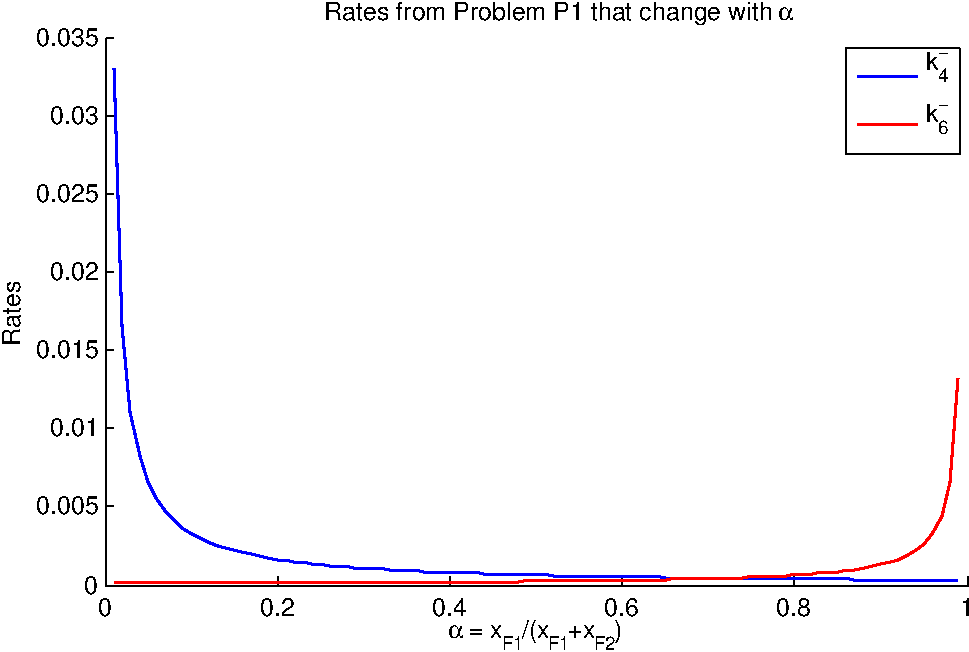
\includegraphics[width=8cm]{img/optimized_rates_alpha_p1.pdf}
		\caption{Backward rates changing continuously with respect to $\alpha$ under objective function P1 for system \eqref{eq:modified_system:reactions}.}
		\label{fig:img_optimized_rates_alpha_p1}
	\end{figure}
		
	Having constant rates for every reaction except those two give several informations:
	
	\begin{my_itemize}
		\item The network is highly flexible, allowing every ratio of final puzzles only by changing two specific backward rates. The non final reactions are kept to an activity low enough so as not to destroy to yield, but still high enough to be able to redistribute the materials when the final reactions are breaking up the final puzzles to converge to a desired ratio. Controlling only the disassembly rate of the two final puzzles is enough to attain any ratio $\alpha$, while optimizing the yield and time to convergence.
		\item All the forward rates are put to their maximum value. This could show that using non-maximum forward rates decreases the convergence rate, but further tests about that hypothesis are necessary. In an informal discussion, G.~Mermoud confirmed similar results in previous works of his with self-assembly processes.
	\end{my_itemize}
	
	Doing the optimization of problem P2, under objective function $f_{min}$ leads to slightly different results. This time the forward rates and backwards rates of reactions 4 and 6 are varying continuously. The forwards rate are not all maximum. Table~\ref{tab:optimized_rates_p2} presents the results for P2.
	
	\begin{table}[h!]
		\begin{center}
		\begin{tabular}{|c|c|c|c|c|c|c|}
			\hline
			\textbf{Reaction} $\mathbf{j}$ & \textbf{1} & \textbf{2} & \textbf{3} & \textbf{4} & \textbf{5} & \textbf{6} \\
			\hline
			\textbf{Optimized} $\mathbf{p^+_j}$ & 0.36 & 0.666 & 1.0 & \textit{continuous} & 0.4705 & \textit{continuous}\\
			\hline
			\textbf{Optimized} $\mathbf{p^-_j}$ & 0.006855 & 0.005027 & 0.00377 & \textit{continuous} &  0.00443 & \textit{continuous} \\
			\hline
		\end{tabular}
		\end{center}
		\caption{Values of optimized rates for varying $\alpha$, under objective function P2 for system \eqref{eq:modified_system:reactions}. \textit{Continuous} rates evolve continuously with respect to $\alpha$.}
		\label{tab:optimized_rates_p2}
	\end{table}
	
	Again with that objective function, the real control of the ratio $\alpha$ is carried on by the last two reactions in the construction of the final assemblies. This time the forward rates have a stronger role in that, but this has yet to be verified that this method is better. See Figure~\ref{fig:img_optimized_rates_alpha_p2} for the continuous variation of rates with respect to $\alpha$.
	
	\begin{figure}[h!]
		\centering
			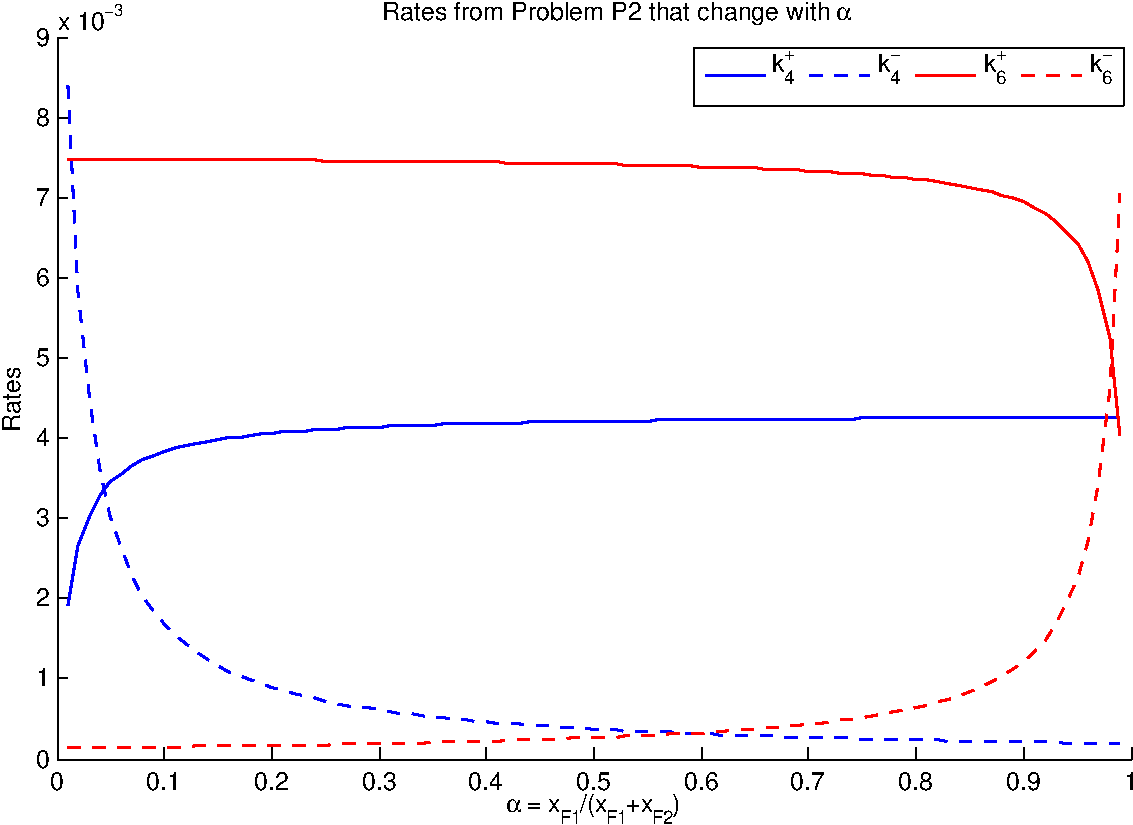
\includegraphics[width=8cm]{img/optimized_rates_alpha_p2.pdf}
		\caption{Forward and backward rates changing continuously with respect to $\alpha$ under objective function P2 for system \eqref{eq:modified_system:reactions}.}
		\label{fig:img_optimized_rates_alpha_p2}
	\end{figure}
	
	\subsection{Comparison between objective functions and strategies} % (fold)
	\label{sub:comparison_between_objective_functions_and_strategies}
	
		To compare the two functions, we plot the time-evolution of the ratio of the final puzzles F1 and F2 for three different $\alpha$: $0.1$, $0.5$ and $0.9$, see Figure~\ref{fig:optim_objfct_comparison} a), c) and e). The horizontal dotted lines show the target ratios and both objective function are shown (plain for P1, dashed for P2).
	
		\begin{figure}[h!]
			\centering
			\subfigure[$\alpha = 0.1$, Linear x axis.] 
			{
				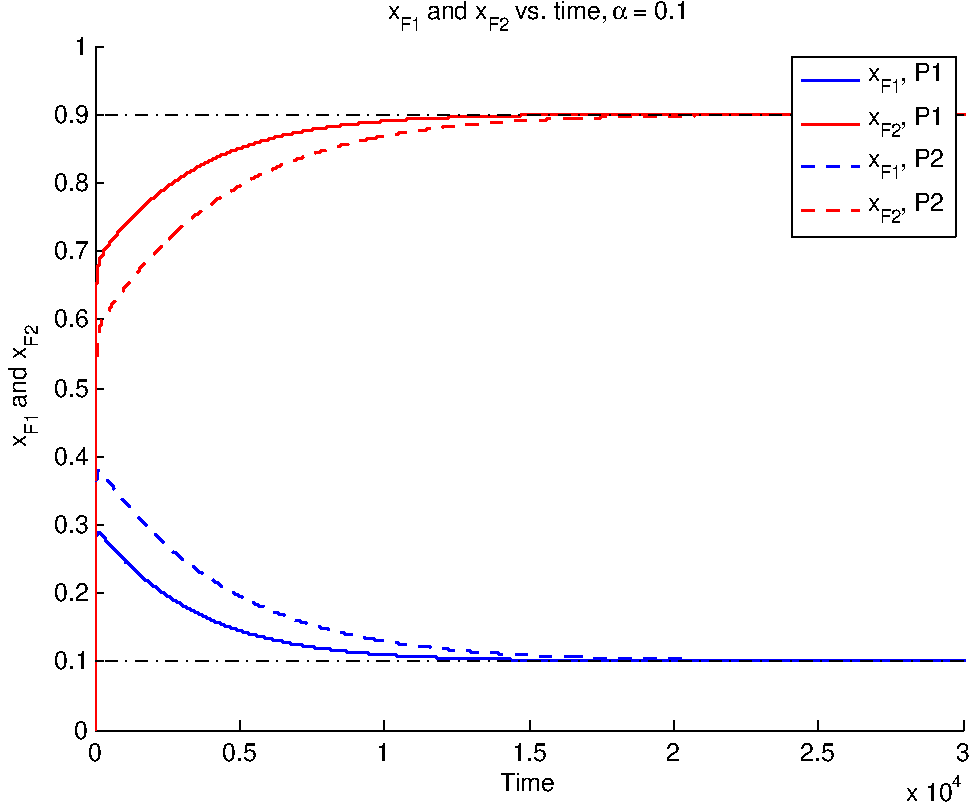
\includegraphics[width=6.5cm]{img/optim_conv_alpha01_lin.pdf}
				\label{fig:optim_objfct_comparison:alpha01_lin}
		 	}
	%		\: % espacement entre figures. \quad \;
			\subfigure[$\alpha = 0.1$, Log x axis.] 
			{
				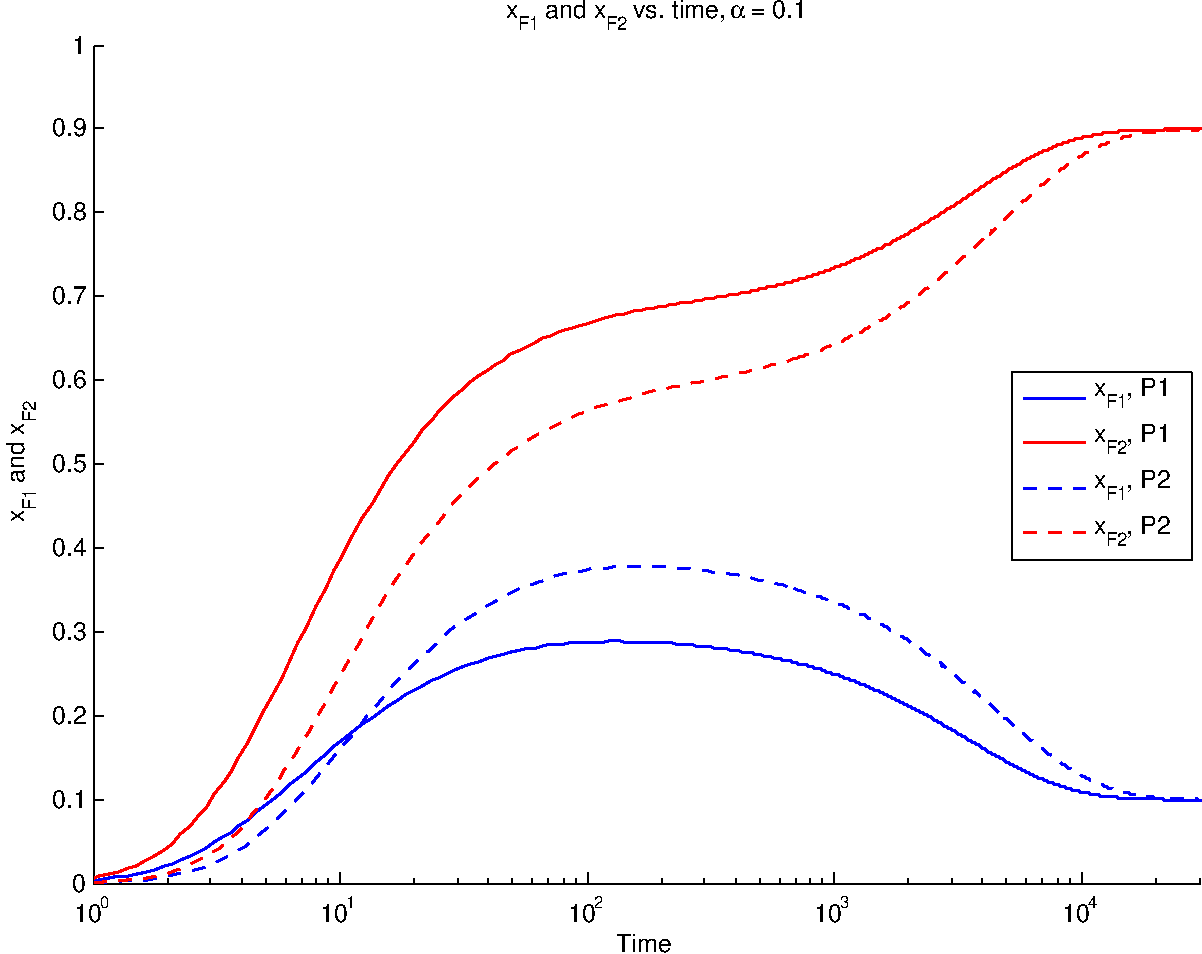
\includegraphics[width=6.5cm]{img/optim_conv_alpha01_log.pdf}
				\label{fig:optim_objfct_comparison:alpha01_log}
		 	}
	%		\: % espacement entre figures. \quad \;
			\subfigure[$\alpha = 0.5$, Linear x axis.] 
			{
				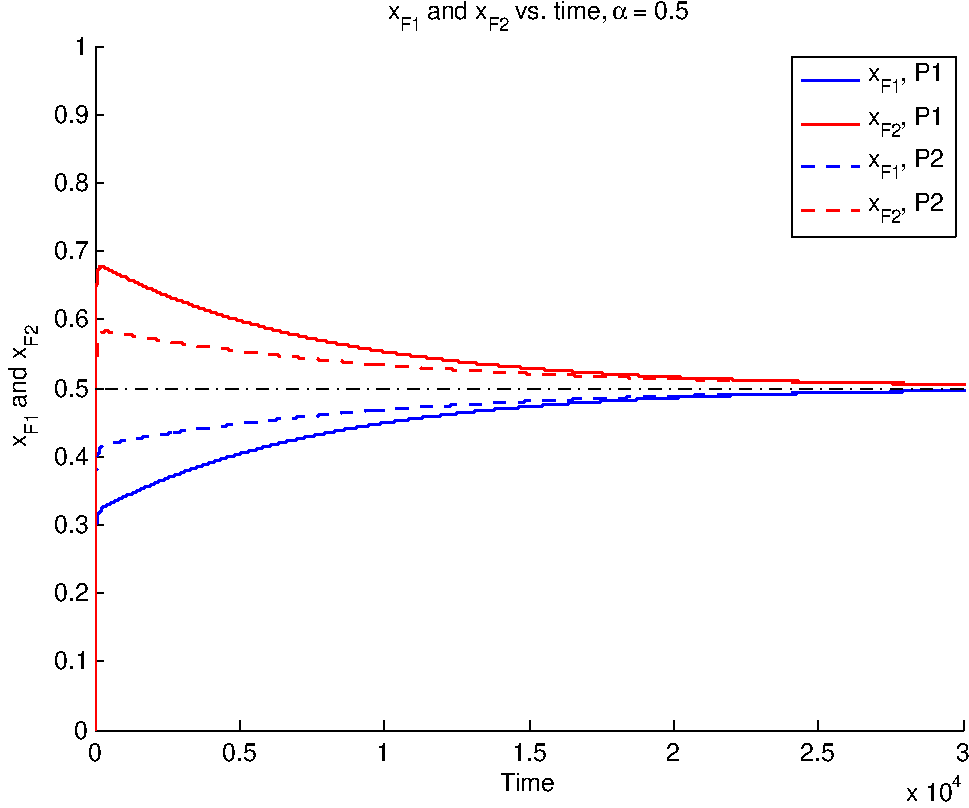
\includegraphics[width=6.5cm]{img/optim_conv_alpha05_lin.pdf}
				\label{fig:optim_objfct_comparison:alpha05_lin}
		 	}
	%		\: % espacement entre figures. \quad \;
			\subfigure[$\alpha = 0.5$, Log x axis.] 
			{
				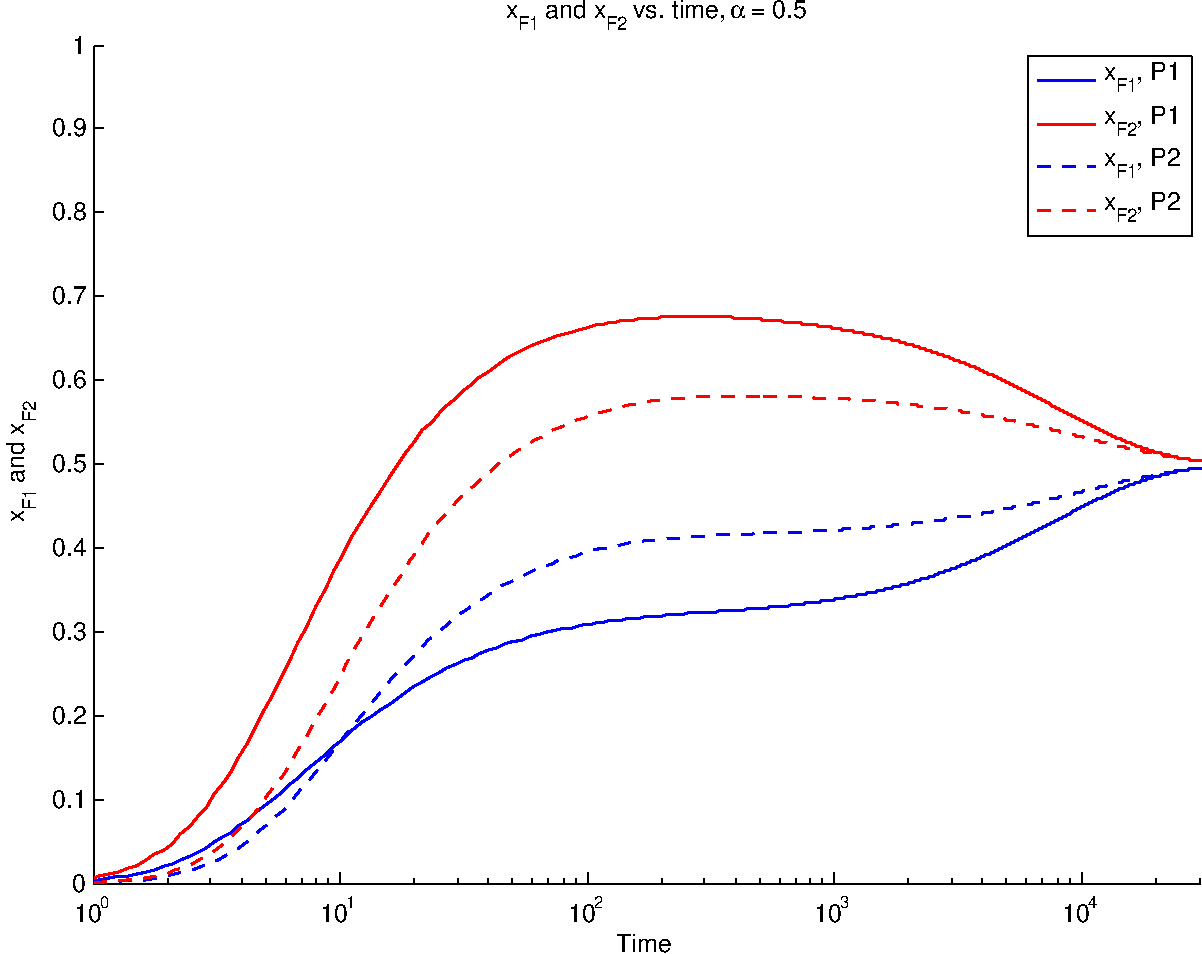
\includegraphics[width=6.5cm]{img/optim_conv_alpha05_log.pdf}
				\label{fig:optim_objfct_comparison:alpha05_log}
		 	}
	%		\: % espacement entre figures. \quad \;
			\subfigure[$\alpha = 0.9$, Linear x axis.] 
			{
				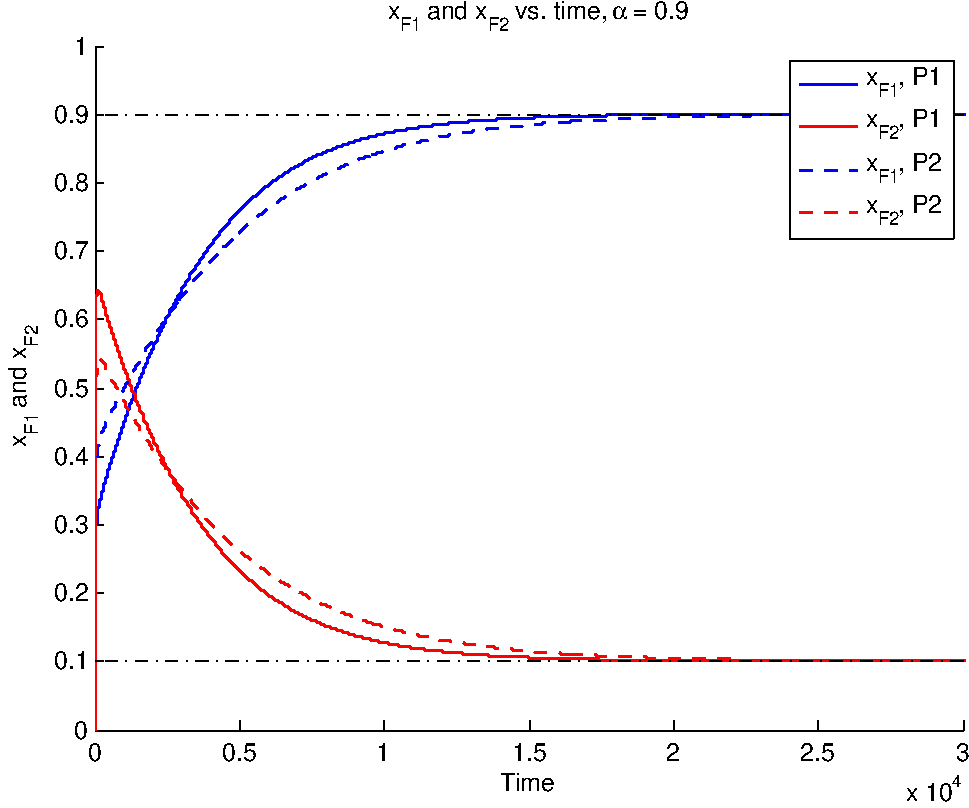
\includegraphics[width=6.5cm]{img/optim_conv_alpha09_lin.pdf}
				\label{fig:optim_objfct_comparison:alpha09_lin}
		 	}
	%		\: % espacement entre figures. \quad \;
			\subfigure[$\alpha = 0.9$, Log x axis.] 
			{
				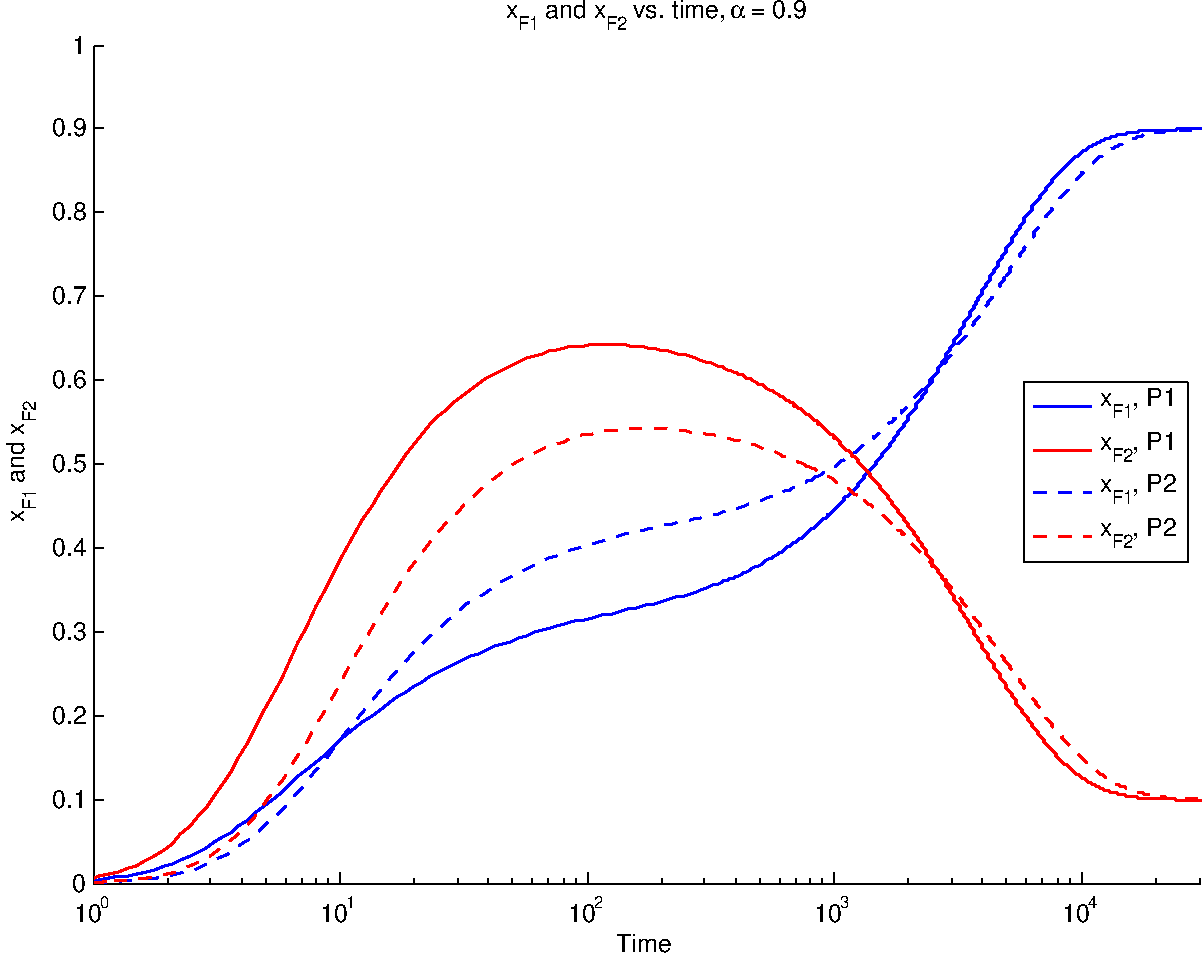
\includegraphics[width=6.5cm]{img/optim_conv_alpha09_log.pdf}
				\label{fig:optim_objfct_comparison:alpha09_log}
		 	}
			\caption{Comparison of convergence of final assemblies over time after optimizing P1 and P2. Time unit is seconds.}
		\label{fig:optim_objfct_comparison} %Caption general
		\end{figure}
		
		
		We see that P1 is converging quicker than P2 to the equilibrium for $\alpha=0.1$ and $\alpha=0.9$, but is slower for $\alpha=0.5$. It is still unclear if it is only due to the values of the forward rates, as hypothesized. The overall speed of convergence is actually pretty slow, especially when trying to produce $50\%$ of both puzzles. This could be problematic, but is in fact linked to the global behavior of the system, as we show now.
	
		Looking at semi-logarithmic plots of the same data, Figure~\ref{fig:optim_objfct_comparison} b), d) and f), we clearly see two regime of convergence:
	
		\begin{my_itemize}
			\item A quick convergence to an unique equilibria, independent of the chosen $\alpha$, till $t=10^2 s$. We hypothesize that this equilibrium depends on the network topology and forward rates.
			\item A ``redistribution'' regime starting from there, which makes the system converge to the final $\alpha$ desired. This regime is much slower than the first one. The final reactions with optimized rates only act during that regime.
		\end{my_itemize}
	
		If we think in the state space of final assemblies, it means that the system first converge quickly to its intrinsic equilibrium, and then moves around slowly due to the redistribution of final puzzles until it arrives to the desired equilibrium.

		This is a very interesting and quite counterintuitive result, as one might think that it would be best to go directly towards the desired equilibrium. The optimization process we use seems to point out that going quickly to the intrinsic equilibrium and then moving from there is a better strategy. Of course, this might be an artifact of the linear optimization we do, so a verification with another optimization process should be performed. This will be done in further works.
	
	% subsection comparison_between_objective_function_and_strategies (end)
	
		% \item The overall convergence to a desired equilibrium 
		% 
		% It means that the optimized way to converge to an equilibrium is the following:
		% 	\begin{my_itemize}
		% 		\item First converge as quickly as possible towards the equilibrium given by the system without backward reactions.
		% 		\item The backward reactions starts their full effect when the number of final puzzles is big enough.
		% 		\item The system slowly converge.
		% 	\end{my_itemize}
	
	\subsection{Online adaptation of the desired final puzzles ratio} % (fold)
	\label{sub:online_adaptation_of_the_desired_final_puzzles_ratio}
		We finish by showing the application of the rate optimization to the ``green manufacturing'' process shortly presented in Section~\ref{sec:definition_of_the_puzzle_test_case}. A ``green manufacturing'' process is a direct application of the flexibility offered by a non-specific assembly task. In that process, we reuse finished products (in our case, final puzzles) in order to create new products, depending on the current demand. We ``recycle'' the products into new ones. This is possible because our system possess the capabilities to create both products, and because we fix what it is supposed to create by optimizing the rates of assembly as shown in this chapter.
		
		We show such an example of online adaptation to a new goal, by simulating the following experiment:
		
		\begin{my_itemize}
			\item Through all this experiment, we use the optimized goals under objective function P1, see Table~\ref{tab:optimized_rates_p1} and Figure~\ref{fig:img_optimized_rates_alpha_p1}.
			\item We initialize the system with a first goal of a $60\%$ ratio of final puzzle F2 ($\alpha=0.4$). We let the system run till $t_1 = 1000 s$.
			\item We change the rates to the one optimized to create a ratio of $99\%$ final puzzle F1 ($\alpha=0.99$). We let the system run till $t_2 = 6000 s$.
			\item We change the rates to a goal of $99\%$ of final puzzle F2 ($\alpha=0.01$). We let the system run till $t_3 = 11000 s$.
			\item We change for the last time the rates for a goal of $50\%$ of each final puzzle ($\alpha=0.5$). We let the system run till $t_4 = 21000 s$.
		\end{my_itemize}
		
		The result is shown in Figure~\ref{fig:optim_online_adaptation}. We see that the system is capable of adapting smoothly to abrupt new commands in the desired targets. It attains the desired ratio when converged. The convergence time is pretty slow when approaching the desired ratio, yet the disruption of the previous steady state occurs quickly. The target of $50\%$ of both puzzles is slower to attain.
				
	\begin{figure}[h!]
		\centering
			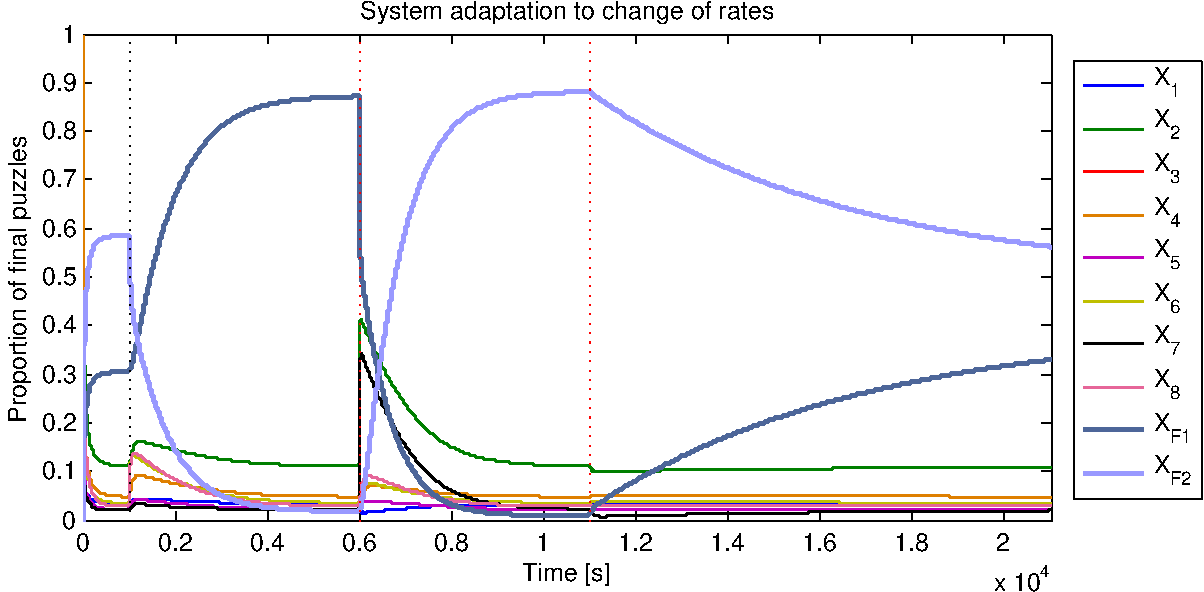
\includegraphics[width=13cm]{img/optim_online_adaptation.pdf}
		\caption{Change of reaction rates during an experiment. System adapts smoothly to the new equilibrium. Rates are changed at the times indicated by the dotted vertical lines. First goal is 60\% of F2, second is 100\% of F1, third is 100\% of F2 and fourth is 50\% of each.}
		\label{fig:optim_online_adaptation}
	\end{figure}
	
	A good result is the speed of adaptation to new commands, and the strong redistribution effect of commands asking for near $100\%$ ratios. We think it is also possible to design a control policy stabilizing quicker to a slow target ($50\%$ for example) by switching between a $100\%$ F1 and a $100\%$ F2 command, slowly damping the oscillations till we attain the desired distribution. This is a similar approach to the one shown in~\cite{Julius:2007p4774, Julius:2008p4775} for the control of switching in \textit{E. Coli}. More tests are still necessary to assess the validity of this process, but the behavior we obtain already offers us a large variety of adaptable behaviors. 
	
	% subsection inline_adaptation_of_the_desired_final_puzzles_ratio (end)
	
% section results_and_limitations (end)




\section{Beyond control, direct optimization of the plan?} % (fold)
\label{sec:beyond_control_direct_optimization_of_the_plan_}
	Can our optimization scheme optimize directly a set of assembly plans? We addressed that problem in Section~\ref{sec:considerations_on_the_assembly_plan}, while speaking about the optimal plans. In his work, Klavins~\cite{Klavins:2007p2600} constructs an optimal assembly plan using graph grammars. This is a discrete optimization, i.e. choosing what reactions to use to build an optimal plan. On the other hand, given optimized rates, it is possible to see if some reactions are promoted or deactivated. This corresponds to a continuous optimization of the assembly plan, effective while the system is behaving. We think our optimization is able to perform such a continuous optimization. We will alter our model in order to test that hypothesis.
	
	We add new assembly steps to create additional pathways to the final assemblies. In addition to plans shown in Figures~\ref{fig:assembly_plans}, we add two new plans, that reuse parts of the old ones, see Figures~\ref{fig:assembly_plans_added}. The new assembly steps are shown in boldface. We call those new plans ``sequential plans'', as they assemble one piece at a time without parallel processes. Our goal is to see how the algorithm treats these new pathways, more precisely if it ``shuts down'' the ones which are not optimal or useful. Remark that we do not consider the case of all possible types of reactions in the system, but only a selected sub-set of them. Using the complete set for the optimization of the plan is let for further work.
	
	\begin{figure}[h!]
		\centering
		\subfigure[New added first final puzzle plan] 
		{
			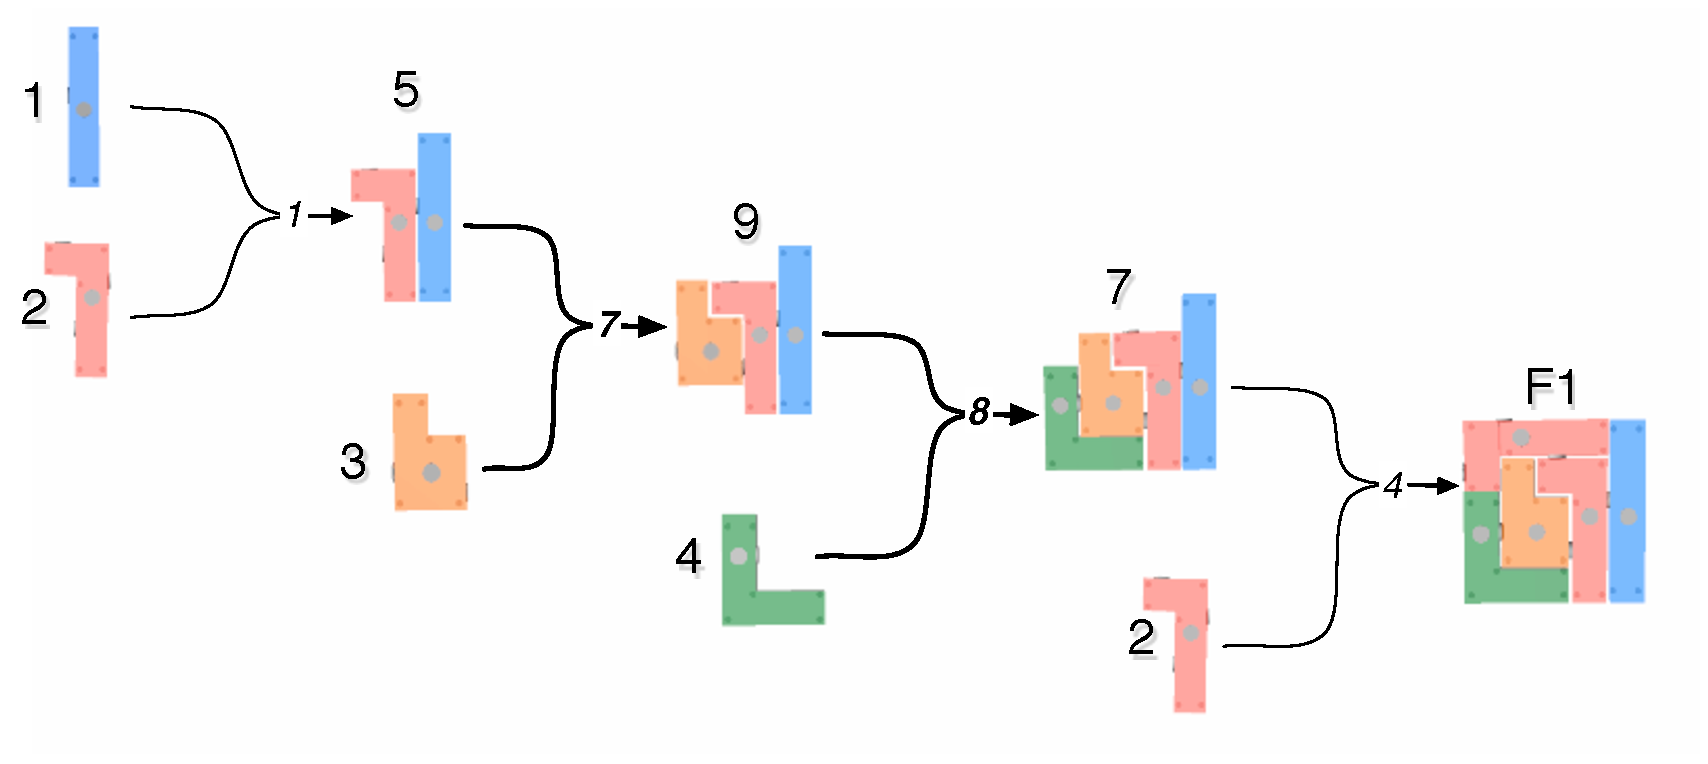
\includegraphics[width=11cm]{img/assembly_plan_f1_added.pdf}
			\label{fig:assembly_plans_added:f1}
	 	}
		\; % espacement entre figures. \quad \;
		\subfigure[New added second final puzzle plan] 
		{
			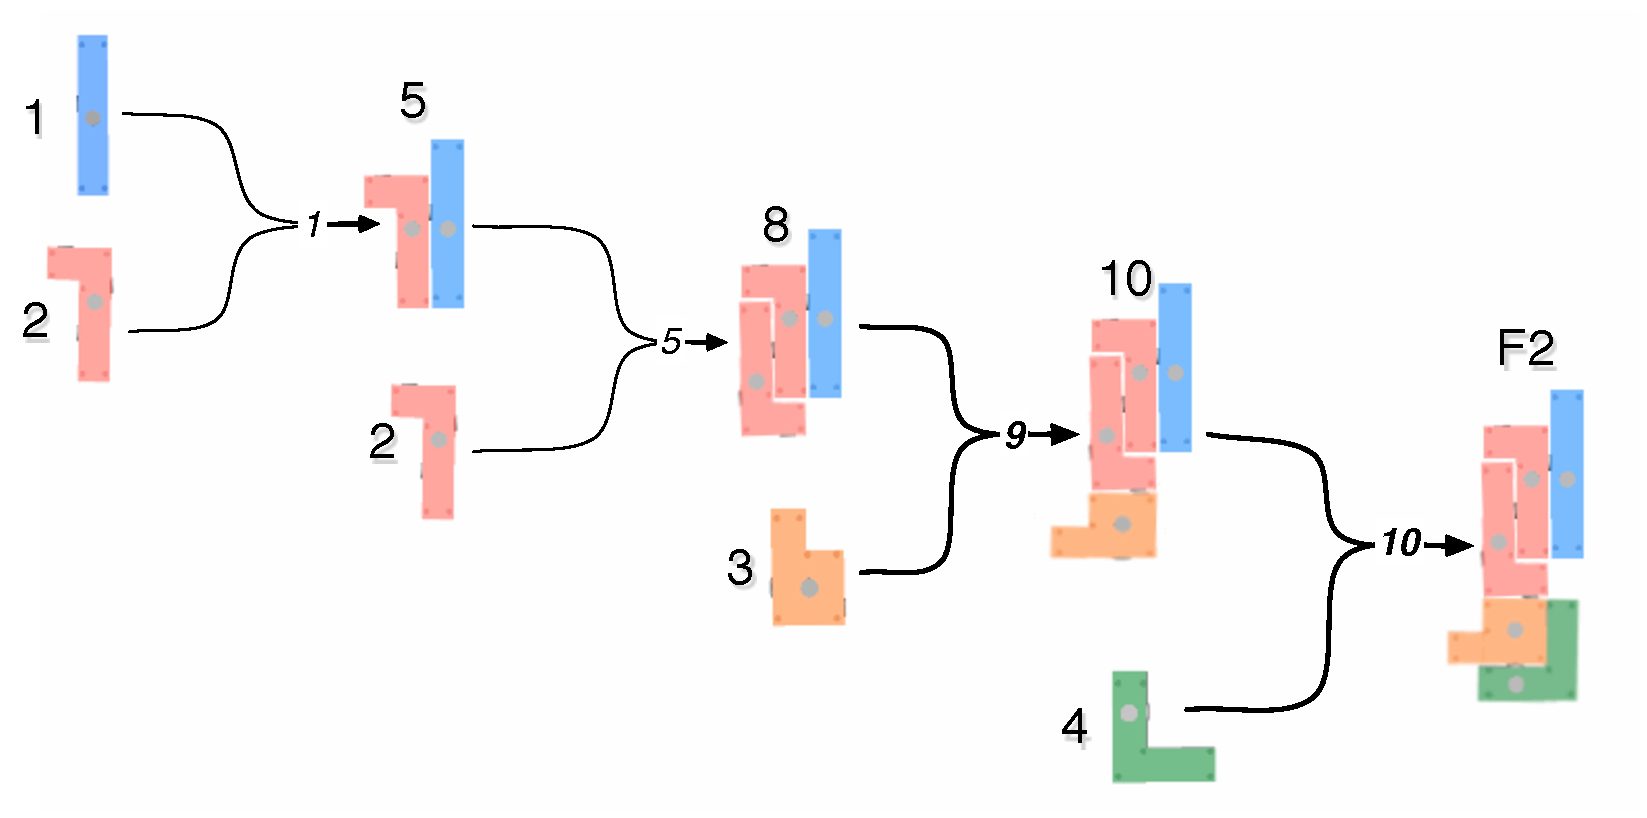
\includegraphics[width=11cm]{img/assembly_plan_f2_added.pdf}
			\label{fig:assembly_plans_added:f2}
	 	}
		\caption{New plans created by adding 4 new assembly steps, written in boldface. We call those plans the ``sequential plans'', as they act by assembling one piece after another without parallel processes.}
	\label{fig:assembly_plans_added} %Cation general
	\end{figure}
		
	The 4 added assembly steps translate into the following reactions to be added to the set \eqref{eq:modified_system:reactions}:
	\begin{eqnarray}
		X_3 + X_5 ~~{\mathop{\rightleftharpoons}_{k_{7}^-}^{k_{7}^+}}~~ X_{9} & \quad & X_3 + X_8 ~~{\mathop{\rightleftharpoons}_{k_{9}^-}^{k_{9}^+}}~~ X_{10} \nonumber \\
		X_4 + X_{9} ~~{\mathop{\rightleftharpoons}_{k_{8}^-}^{k_{8}^+}}~~ X_7 & & X_4 + X_{10} ~~{\mathop{\rightleftharpoons}_{k_{10}^-}^{k_{10}^+}}~~ X_{F2}
	\label{eq:reactionsExp}
	\end{eqnarray}
	
	With these added reactions, the ODE equations for the system are:
	
	\begin{equation} \label{eq:ODEequationsExp}
		\left\lbrace\begin{array}{lll}
			\dot{x}_1 &=& - k_1^+ x_1 x_2 + k_1^- x_5    \\
			\dot{x}_2 &=& - k_1^+ x_1 x_2 - k_5^+ x_2 x_5 - k_4^+ x_2 x_7 + k_1^- x_5 + k_{5}^- x_8 + k_4^- x_{F1}  \\
			\dot{x}_3 &=& - k_2^+ x_3 x_4 + k_2^- x_6 - k_{7}^+ x_3 x_5 + k_{7}^- x_{9} - k_{9}^+ x_3 x_8 + k_{9}^- x_{10}  \\
			\dot{x}_4 &=& - k_2^+ x_3 x_4 + k_2^- x_6 - k_{8}^+ x_4 x_9 + k_{8}^- x_{7} - k_{10}^+ x_4 x_{10} + k_{10}^- x_{F2}  \\
			\dot{x}_5 &=& 	k_1^+ x_1 x_2 - k_1^- x_5 - k_3^+ x_5 x_6 + k_3^- x_7 - k_5^+ x_2 x_5 \\
			 &  & + k_{5}^- x_8 - k_{7}^+ x_3 x_5 + k_{7}^- x_{9}  \\
			\dot{x}_6 &=&   k_2^+ x_3 x_4 - k_2^- x_6 - k_3^+ x_5 x_6 + k_3^- x_7 - k_{6}^+ x_6 x_8 + k_{6}^- x_{F2}  \\
			\dot{x}_7 &=& 	k_3^+ x_5 x_6 - k_3^- x_7 - k_4^+ x_2 x_7 + k_4^- x_{F1} + k_{8}^+ x_4 x_9 - k_{8}^- x_{7}   \\
			\dot{x}_8 &=& 	k_5^+ x_2 x_5 - k_{5}^- x_8 - k_{6}^+ x_6 x_8 + k_{6}^- x_{F2} - k_{9}^+ x_3 x_8 + k_{9}^- x_{10} \\
			\dot{x}_9 &=& 	k_{7}^+ x_3 x_5 - k_{7}^- x_{9} - k_{8}^+ x_4 x_{9} + k_{8}^- x_{7}   \\
			\dot{x}_{10} &=& k_{9}^+ x_3 x_8 - k_{9}^- x_{10} - k_{10}^+ x_4 x_{10} + k_{10}^- x_{F2}   \\
			\dot{x}_{F1} &=& k_4^+ x_2 x_7 - k_4^- x_{F1}  \\
			\dot{x}_{F2} &=& k_{6}^+ x_6 x_8 - k_{6}^- x_{F2} + k_{10}^+ x_4 x_{10} - k_{10}^- x_{F2} \\
		\end{array}
		\right.
	\end{equation}

	Like system \eqref{eq:ODEequations}, this system can be written in
	the form \eqref{eq:matrixODE}.  In this case, the vector of
	complexes is defined as
		
	\begin{eqnarray}
		\mathbf{y(x)} = &&[x_1 x_2,~x_5,~x_3 x_4,~x_6,~x_2 x_7,~ x_{F1},~ x_5
		x_6,~ x_7,~ x_2 x_5, \nonumber \\
		&& x_8,~ x_6 x_8,~ x_{F2},~ x_3 x_5,~ x_{9},~ x_4 x_{9},~ x_3
		x_8,~ x_{10},~ x_4 x_{10}]^T~. \label{eq:yExp}
	\end{eqnarray}

	%[diff labels for S, K, y in expanded system?]

	One set of conservation constraints on the piece quantities in this system is:
	\begin{equation}\label{eq:consExp}
		\left\lbrace\begin{array}{lll}
			x_1+x_5+x_7+x_8+x_{F1}+x_{F2}+x_{9}+x_{10} &=& N_5 \\
			x_2+x_5+x_7+2 x_8+2 x_{F1}+2 x_{F2}+x_{9}+2 x_{10} &=& N_6 \\
			x_3+x_6+x_7+x_{F1}+x_{F2}+x_{9}+x_{10} &=& N_7\\
			x_4 + x_6 + x_7 + x_{F1} + x_{F2} &=& N_8 
		\end{array}
		\right.
	\end{equation}
	
	where $N_i$, $i=5,...,8$, are computed from the initial piece
	quantities.
	
	\subsection{Optimized rates and induced effective plan} % (fold)
	\label{sub:optimized_rates}
		We apply our optimization procedure with Problem P1 and P2 as before. The results for the convergence are shown in Figure~\ref{fig:exp_optim_objfct_comparison}. As Problem P2 is quicker in general and shows more interest dynamics, we will only study it for the rest of this section.
		
			\begin{figure}[h!]
				%\centering
				\subfigure[$\alpha = 0.1$, Log x axis.] 
				{
					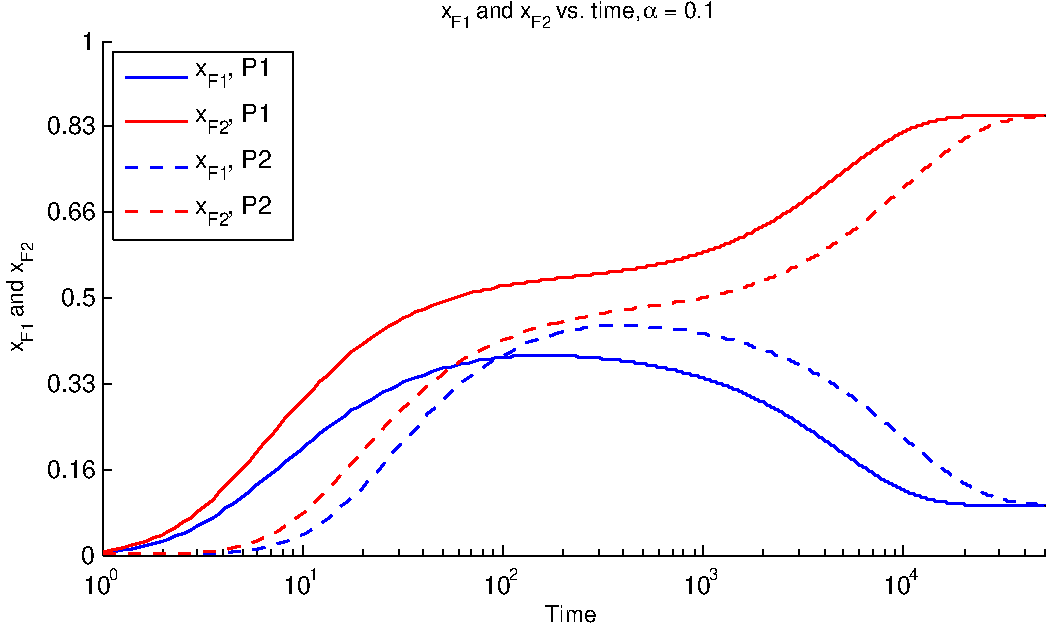
\includegraphics[width=7.2cm]{img/optim_exp_conv_alpha01.pdf}
					\label{fig:exp_optim_objfct_comparison:alpha01_log}
			 	}
		%		\: % espacement entre figures. \quad \;
				\subfigure[$\alpha = 0.5$, Log x axis.] 
				{
					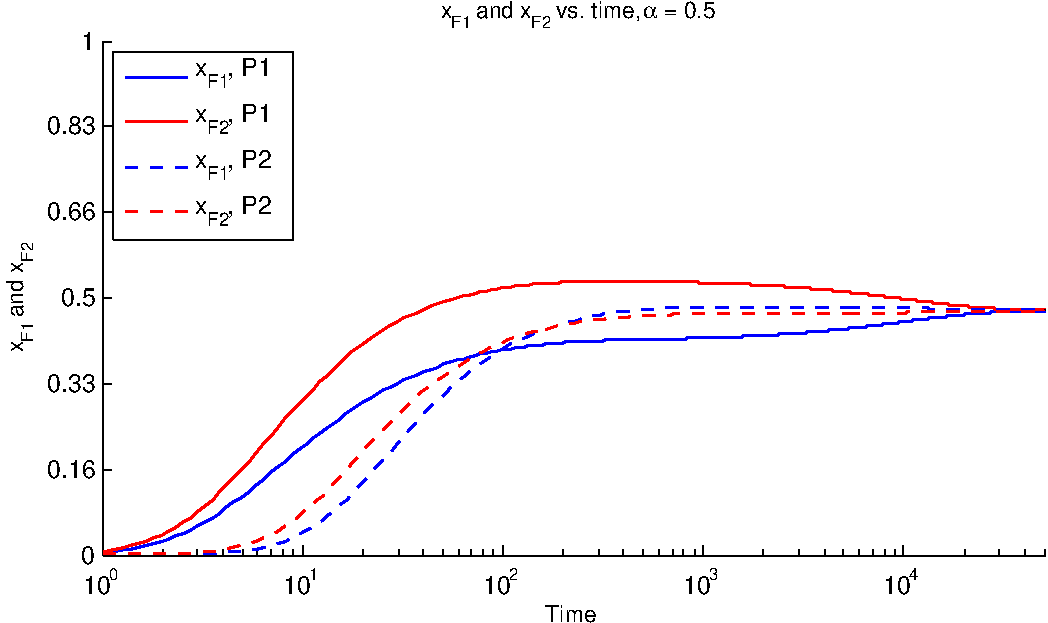
\includegraphics[width=7.2cm]{img/optim_exp_conv_alpha05.pdf}
					\label{fig:exp_optim_objfct_comparison:alpha05_log}
			 	}
		%		\: % espacement entre figures. \quad \;
				\begin{center}
					\subfigure[$\alpha = 0.9$, Log x axis.] 
					{
						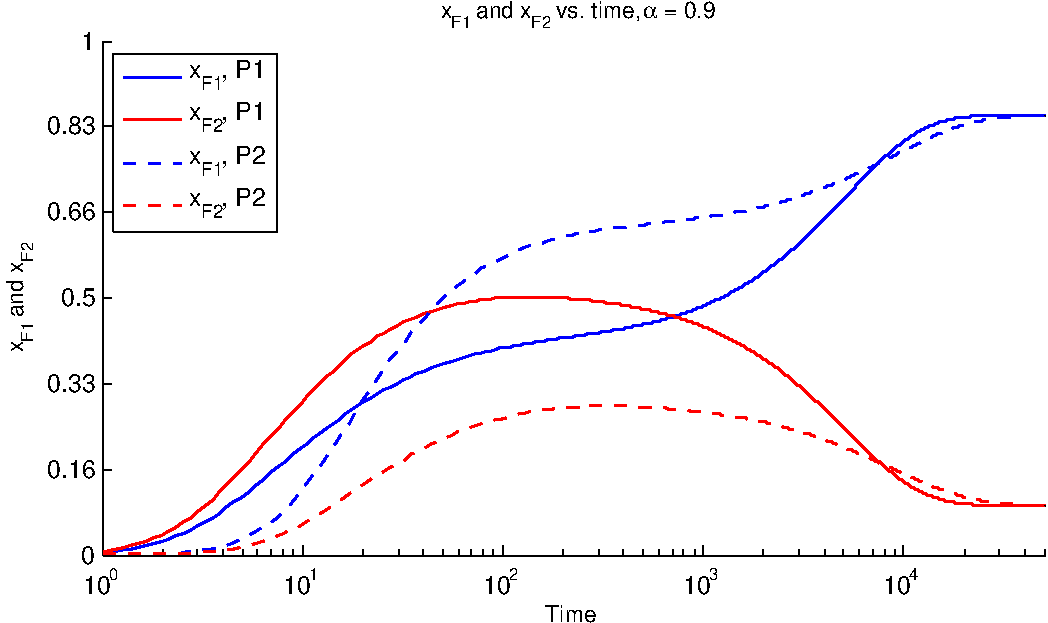
\includegraphics[width=7.2cm]{img/optim_exp_conv_alpha09.pdf}
						\label{fig:exp_optim_objfct_comparison:alpha09_log}
			 			}
				\end{center}
				\caption{Expanded system. Comparison between the two objective functions P1 and P2 when showed with semi-logarithmic x axis.}
			\label{fig:exp_optim_objfct_comparison} %Caption general
			\end{figure}
		
		The resulting probabilities $p_i^+, p_i^-$ for problem P2 are nearly all continuously varying. The only exceptions are $p_3^+$, $p_6^+$ and $p_9^+$ which are all at $1.0$. The variation of the rates for the values of $\alpha$ are shown in Figure~\ref{fig:exp_optim_varying_rates}.
		
		\begin{figure}[h!]
			\centering
			\subfigure[Forward rates varying continuously] 
			{
				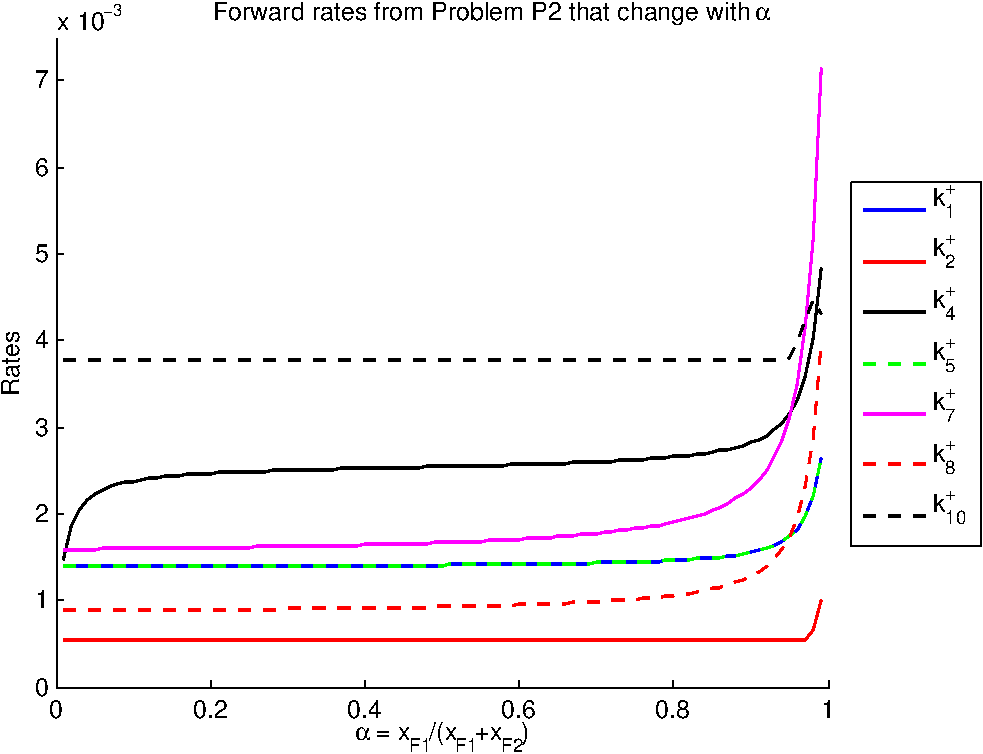
\includegraphics[width=10cm]{img/optim_exp_forward_rates.pdf}
				\label{fig:exp_optim_varying_rates:forward}
		 	}
	%		\: % espacement entre figures. \quad \;
			\subfigure[Backward rates varying continuously] 
			{
				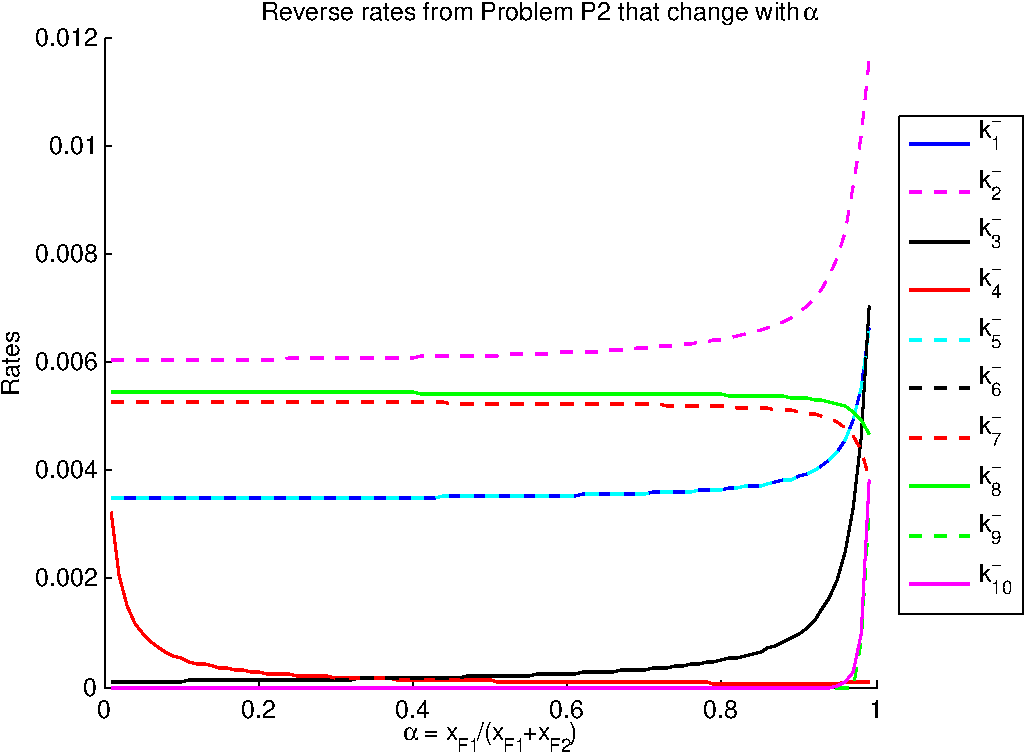
\includegraphics[width=10cm]{img/optim_exp_backward_rates.pdf}
				\label{fig:exp_optim_varying_rates:backward}
		 	}
	%		\: % espacement entre figures. \quad \;
				\caption{Optimized rates of expanded system under problem P2, for $\alpha \in {0.01, 0.99}$. Remark: $k_6^-$ curve is the same as $k_3^-$.}
		\label{fig:exp_optim_varying_rates} %Caption general
		\end{figure}
		
		Looking at the values of the rates at specific positions, we can make observation on the actual plan promoted by the optimization. The reactions, though still present, will be promoted or deactivated when their corresponding forward and backward rates are modified. This corresponds to a continuous optimization of the plan, in contrast with a discrete optimization performed by Klavins\cite{Klavins:2007p2600}.
		
		In general, the value of the rates show the following hierarchy between reactions and pathways:
		\begin{itemize}
			\item $k_2^+$ is small and $k_2^-$ is big compared to other rates. This deactivates Reaction 2.
			\item To compensate the absence of piece 6, the sequential pathways represented by reactions 7 and 8 for F1 and reactions 9 and 10 for F2 are really active.
			\item The small amount of pieces 6 that would result from breaking of assemblies are quickly reuse via the reactions 3 and 6, which have of full forward rate, or destroyed by the backward rate of reaction 2.
		\end{itemize}
		
		We see three different regimes for the rates, and the resulting continuous assembly plans:
		\begin{my_enumerate}
			\item Near $\alpha=0.1$, the only changing rates are $k_4^+$ and $k_4^-$. They are changing toward a deactivation of Reaction 4, which is the only one creating F1 puzzles. The network then automatically tends to create more F2 puzzles, which seems to be a constant characteristic of the system we are studying.
			\item Between $\alpha=0.2$ and $\alpha = 0.8$, the rates $k_4^+$ and $k_6^-$ seems to have to most effect. They act by promoting the creation of F1 and slowing the creation of F2. During that period, the networks tends to produce a $50\%$ ratio by itself, as shown by the convergence profile in Figure~\ref{fig:exp_optim_objfct_comparison:alpha05_log}: the first convergence arrives close to a $50\%$, no redistribution is needed (to compare with Figure~\ref{fig:optim_objfct_comparison:alpha05_log} of the previous system)
			\item Near $\alpha = 0.9$, the behavior changes dramatically. Reactions 7, 8 and 4, leading to the creation of F1 are promoted extensively (increase in forward rate, decrease in backward rate). At the same moment, reactions 6 and 10, creating F2, are deactivated. This promotes the creation of F1 puzzles.
		\end{my_enumerate}
		
		We see then that this optimization works with these general tendencies:
		
		\begin{my_itemize}
			\item Remove assembly 6 from the possible pool of pieces, to liberate all initial pieces for other reactions. This means removing the initial plans we were using an use the new introduced one, see Figure~\ref{fig:assembly_plans_added}
			\item Use the sequential steps to create the final puzzles. This is a counter-intuitive results, but it may be linked to an added flexibility with having a large pool of initial pieces, that can be used at precise assembly steps without temporal dependences between reactions.
			\item Modify the reactions leading to the final assemblies to change the ratio, and do not touch the ``general'' part of the system. This is in agreement with the behavior we observed in last section.
			\item As the system is more prone to create F2 than F1, it is easier to control the system in one direction than the other. To create a big ratio of F1, the overall behavior of the system is changed, leading to a nearly new plan. This plan correspond to the sequential one we added in Figure~\ref{fig:assembly_plans_added:f1}.
		\end{my_itemize}
		
	% subsection optimized_rates (end)
	
	So in conclusion, it is possible to get insights into the kind of behaviors and continuous plans promoted by the optimization. The algorithm promoted the use of sequential plans, with the addition of ``rewiring'' the system when the goal to attain is in contradiction with the intrinsic behavior of the system (e.g. to create the big ratio of F1).
	
	These results are not that intuitive, i.e. one would think that using parallel assembly steps is more efficient for the convergence time. But comparing the results, we see that the ``sequential plan'' is much quicker for $\alpha=0.5$, and slightly worse for the two others ($4\cdot 10^4~seconds\mbox{ instead of } 3 \cdot 10^4~seconds$).
	However, it has to be checked that such an optimization would give similar results for a more complicated set of assembly plans, especially the ``full set assembly plan'' consisting of all possibles reactions of the system.
% section beyond_control_direct_optimization_of_the_plan_ (end)

% chapter chemical_reaction_networks_control_and_design (end)

% % empty page
\pagebreak
\thispagestyle{empty}
\begin{center}\tiny \sc This page intentionally left blank.\end{center}
\pagebreak

\chapter{Augmented assembly implementation} % (fold)
\label{cha:augmented_assembly_implementation}
	\section{Top-bottom approach} % (fold)
\label{sec:top_bottom_approach}
	This chapter will cover the last step in our methodology: going back from the modified model to the physical system, while applying the introduced modifications.

	This is a Top-bottom approach, which is of growing interests nowadays. This method becomes interesting when the behavior of the low-level parts is hard to create, when the global behavior does not simply follow from the behavior of the low-level parts or when we want to low-level parts to follow directives given at a higher level.

	In our case, our problem is that we do not know how to modify the behavior of the low-level parts (i.e. the robots and pieces and their interactions) so as to create a high-level goal. When working on the mathematical model level, we can define our high-level goals more easily.

	The main difficulty of this approach is to create a mapping from the high-level to the low-level.
% section top_bottom_approach (end)

\section{Rates mapping} % (fold)
\label{sec:rates_mapping}
	In our case, this problem is actually simpler, because we have a direct dependance between rates in the mathematical model and behavior of the robots.
	
	Especially, we created a bidirectional relation between the stochastic constant rates of our mathematical model and physical capacities or behavior of our robots and pieces. The mapping from the model to the physical system is thus straightforward:
	\begin{description}
		\item[Backward probability $p_i^-$:] A robot carrying an assembly draws a random number at each timestep and compare it to the $p_i^-$ corresponding to its carried assembly $i$. Precisely:
		
		\textit{if} $U(0,1) < p_i^-\cdot T \rightarrow $ \textit{disasssemble assembly} $i$.
		
		where $T$ is the timestep of the physical simulation. This is needed because $p_i^-$ is a backward rate per second.
		\item[Forward probability $p_i^+$:] As shown in Equation~\eqref{eq:forward_rate_opt}, this probability is used when an assembly is starting. Before actually doing the assembly, a random number is drawn and compared to it:
		
		\textit{if} $U(0,1) < p_i^+\cdot T \rightarrow $ \textit{perform assembly step} $i$.
	\end{description}
	
	When a disassembly is triggered, the carrying robot drops one of the assemblies on the ground and resume searching with the remaining carried assembly. This dropped assembly should then be grabbed by another robot in order to be attached again.
	
	These behavior should directly create the change of rates needed for the modified mathematical model.
	
	When such a bidirectional mapping is not that easily available, we have to discover that mapping. A possibility would be to create an iterative process between a modification of low-level parameters and a measure of the resulting rate modification in the model.
% section rates_mapping (end)

\section{Augmentation results and implications} % (fold)
\label{sec:augmentation_results_and_implications}

	We choose to implement the set of optimized probabilities shown in Table~\ref{tab:optimized_probabilities_augmented}. It has been found by solving problem P1 in Section~\ref{sec:results_and_limitations}.
	
	\begin{table}
		\begin{center}
		\begin{tabular}{|c|c|c|c|c|c|c|c|}
			\hline
			\multicolumn{2}{|c|}{\textbf{Reaction} $\mathbf{j}$} & \textbf{1} & \textbf{2} & \textbf{3} & \textbf{4} & \textbf{5} & \textbf{6} \\
			\hline
			 	& $\alpha = 0.01$ & \multicolumn{6}{c|}{} \\
			$\mathbf{p^+_j}$ & $\alpha = 0.5$ & \multicolumn{6}{c|}{1.0} \\
				& $\alpha = 0.99$ & \multicolumn{6}{c|}{} \\
			\hline
			& $\alpha = 0.01$ &  &  &  & 0.033074 &  & 0.000134 \\
			$\mathbf{p^-_j}$ & $\alpha = 0.5$ & 0.018852 & 0.007541 & 0.003770 & 0.000661 & 0.009426 & 0.000265 \\
			& $\alpha = 0.99$ &  &  &  &  0.000334 &  & 0.013229 \\
			\hline
		\end{tabular}
		\end{center}
		\caption{Set of optimized probabilities used for the Top-down mapping. Reactions from system \eqref{eq:modified_system:reactions}.}
		\label{tab:optimized_probabilities_augmented}
	\end{table}
	
	\subsection{Stochastic model} % (fold)
	\label{sub:stochastic_model}
		We start by verifying the behavior with the stochastic simulation of our model with backward rates. We modify Equation~\eqref{eq:ode_transportersimple} to add the backward reactions while still modeling the robots and free pieces. Our model takes into account the dropped pieces when a disassembly occurs. The results for 1 puzzle are shown in Figure~\ref{fig:stoch_augm_1puzzle}. The results are similar for 3 puzzles, so we do not show them here.
		
			\begin{figure}[h!]
				%\centering
				\subfigure[$\alpha = 0.01$] 
				{
					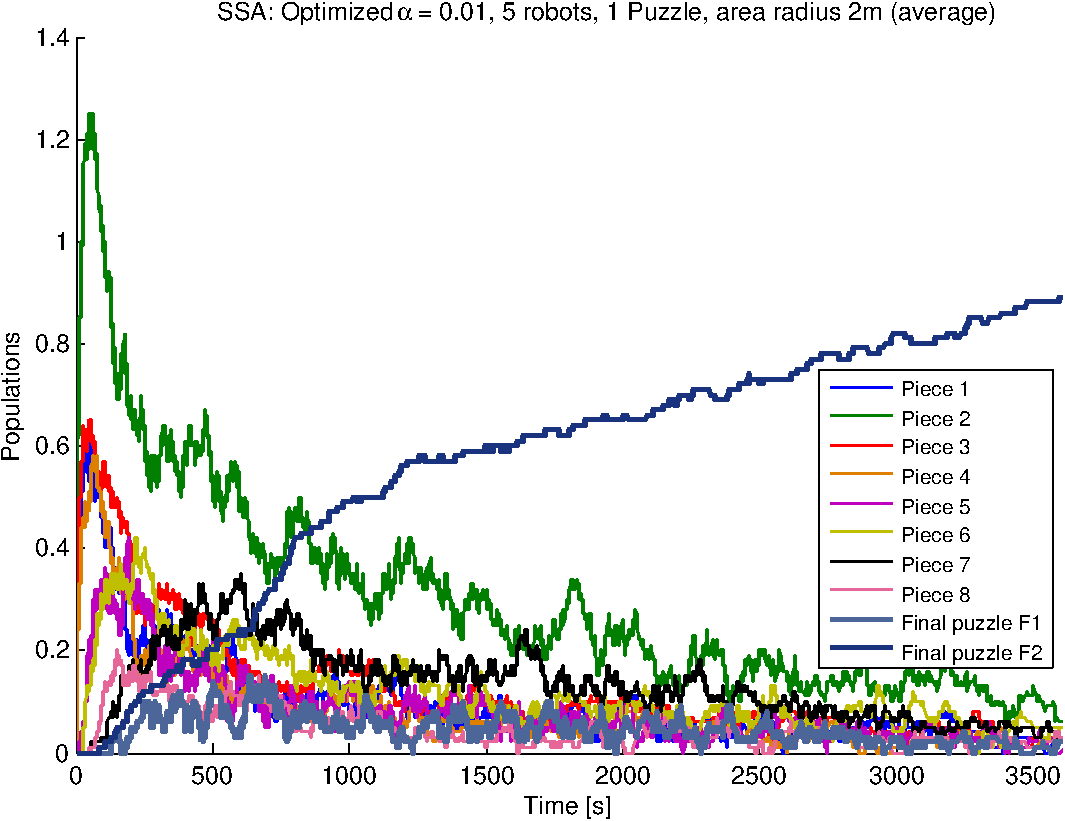
\includegraphics[width=7.2cm]{img/augm_stoch1puzzle_5robots_alpha001.pdf}
					\label{fig:stoch_augm_1puzzle:alpha001}
			 	}
		%		\: % espacement entre figures. \quad \;
				\subfigure[$\alpha = 0.5$] 
				{
					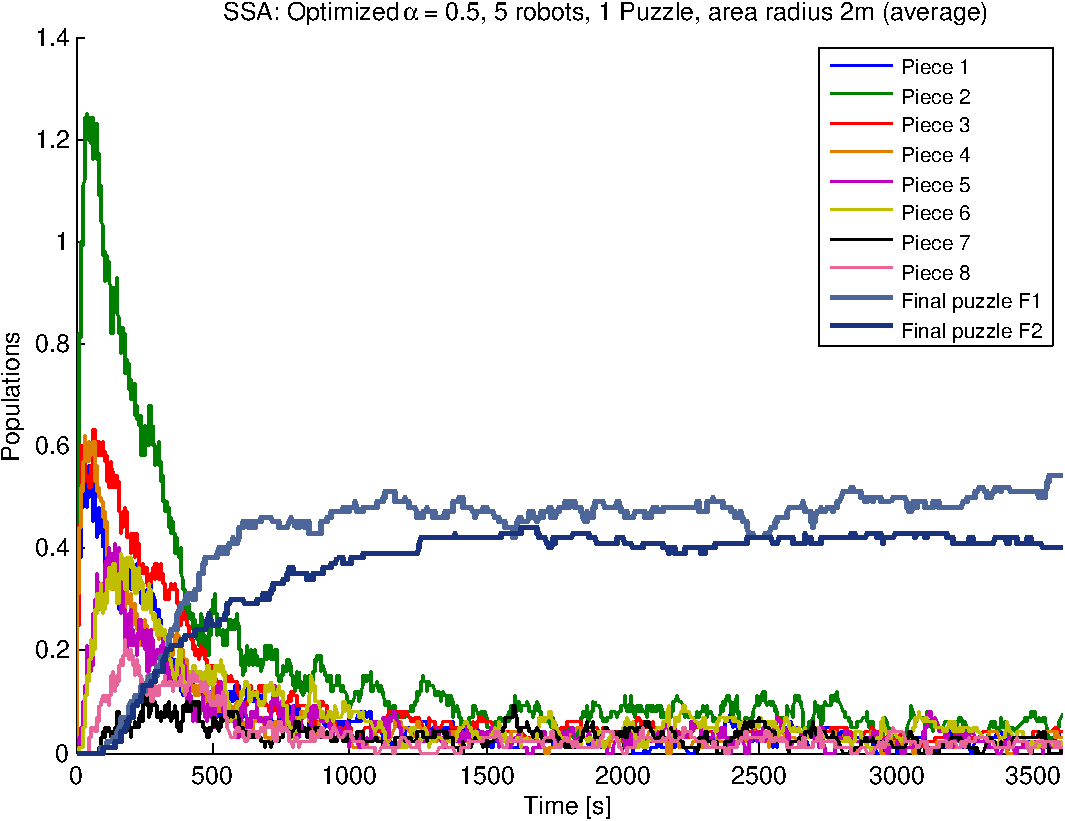
\includegraphics[width=7.2cm]{img/augm_stoch1puzzle_5robots_alpha05.pdf}
					\label{fig:stoch_augm_1puzzle:alpha05}
			 	}
		%		\: % espacement entre figures. \quad \;
				\begin{center}
					\subfigure[$\alpha = 0.99$] 
					{
						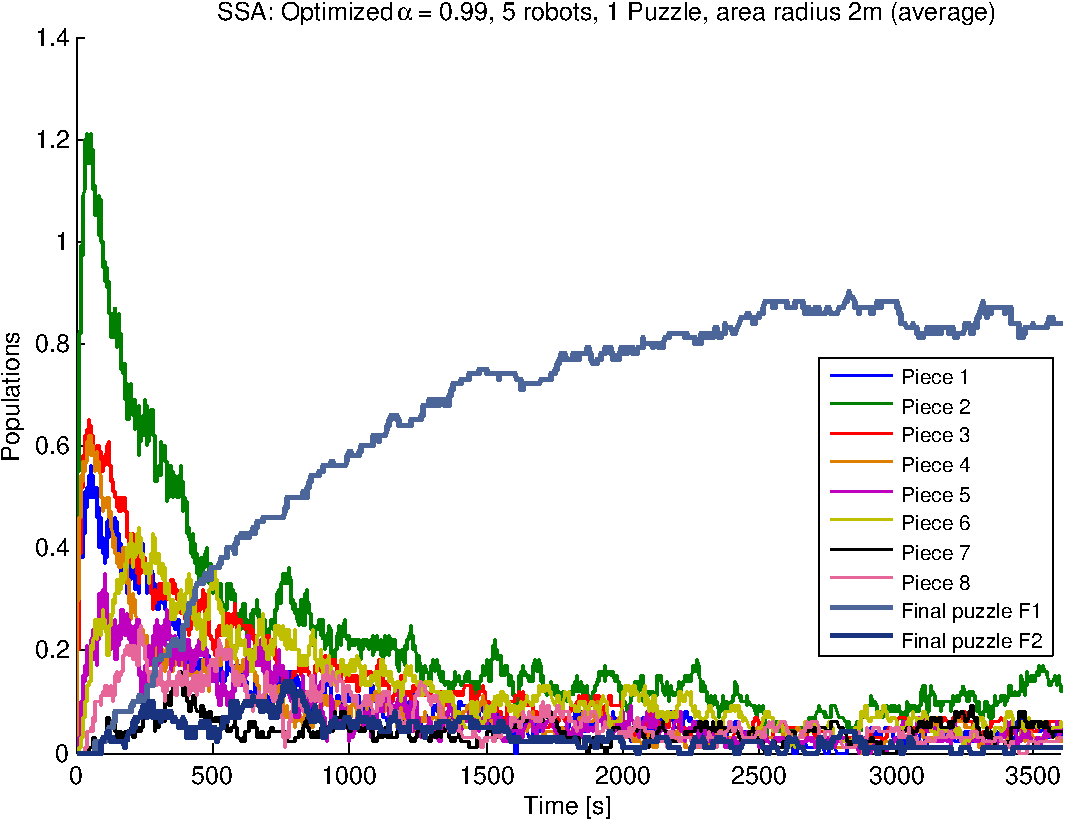
\includegraphics[width=7.2cm]{img/augm_stoch1puzzle_5robots_alpha099.pdf}
						\label{fig:stoch_augm_1puzzle:alpha099}
				 	}
					
				\end{center}
				\caption{Stochastic simulation of the Augmented system, for 1 puzzle and 5 robots.}
			\label{fig:stoch_augm_1puzzle} %Caption general
			\end{figure}
		
		According to these simulations, the optimized rates for the simplified system \eqref{eq:modified_system:reactions} translates into the same global optimized behavior when used on the complete system with robots and free pieces. It manages to create the target ratio $\alpha$ quite successfully. This is a good thing, as it shows that we have a full loop between the physical system and the optimization of the model. We see that, because of the low number of pieces available, there are still quite a lot of non final puzzles in the system. 
	% subsection stochastic_model (end)
	
	\subsection{Physical simulation} % (fold)
	\label{sub:physical_simulation}
		
		As explained earlier, we augmented the system by adding the capacity to break assemblies and grab mid-assemblies lying on the floor. We then use the optimized probabilities of Table~\ref{tab:optimized_probabilities_augmented} before running our simulations.
		
		\subsubsection{The carried pieces discrepancy} % (fold)
		\label{ssub:the_carried_pieces_discrepancy}
		
		Our first result is an experiment with $\alpha=0.01$, using 5 robots and 5 pieces. We run 100 experiments, using the same methodology as explained in Section~\ref{ssub:experiment_3_5_pieces_and_5_robots_final_puzzles_f1_and_f2}, for a maximum of 10 minutes. The results are shown in Figure~\ref{fig:img_augm_res1puzzle_5robots}.
		
		\begin{figure}[h]
			\centering
				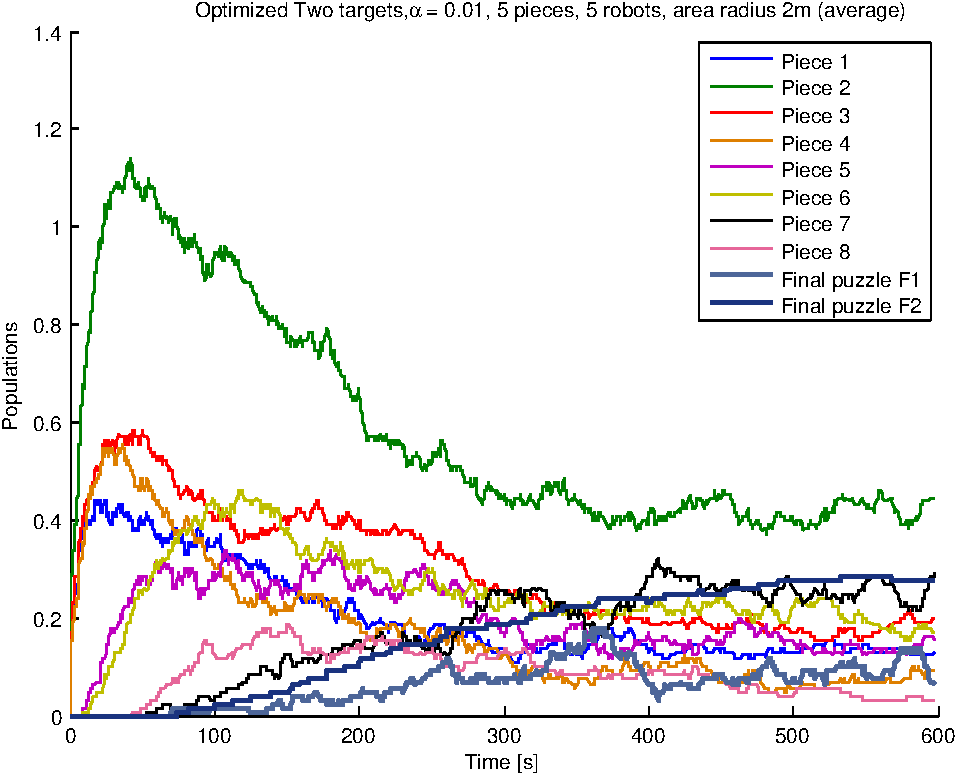
\includegraphics[width=8cm]{img/augm_res1puzzle_5robots_alpha001.pdf}
			\caption{Results of the augmented system with optimized rates for $\alpha=0.01$. Problem of carrying of pieces.}
			\label{fig:img_augm_res1puzzle_5robots}
		\end{figure}
		
		This is quite disappointing, as it does not converge to our desired values, even if we do not run the system for a long time. The biggest problem is the amount of free piece 2: they are more abundant than final assemblies.
		
		Studying visually the behavior in simulation, we discovered that this problem is due to the re-carrying of pieces dropped during a disassembly. When few robots are available, the time till a piece is carried again can be in the same order of magnitude than the time between two assemblies. Yet when constructing our model for the optimization, we assumed that the pieces would be carried very quickly (Section~\ref{sub:changes_on_our_models}). This hypothesis is thus pretty important as its effect shows it here.
		
		In order to correct that, we add 3 robots to the arena, which ensure that the time to re-carrying of pieces is small.
		We then compare the results of this new physical simulation to the stochastic simulation of the same experiment in Figure~\ref{fig:img_augm_stochphys_alpha001}. Again we do 100 experiments, of 10 minutes each for a target value $\alpha=0.01$.

		\begin{figure}[h]
			\centering
				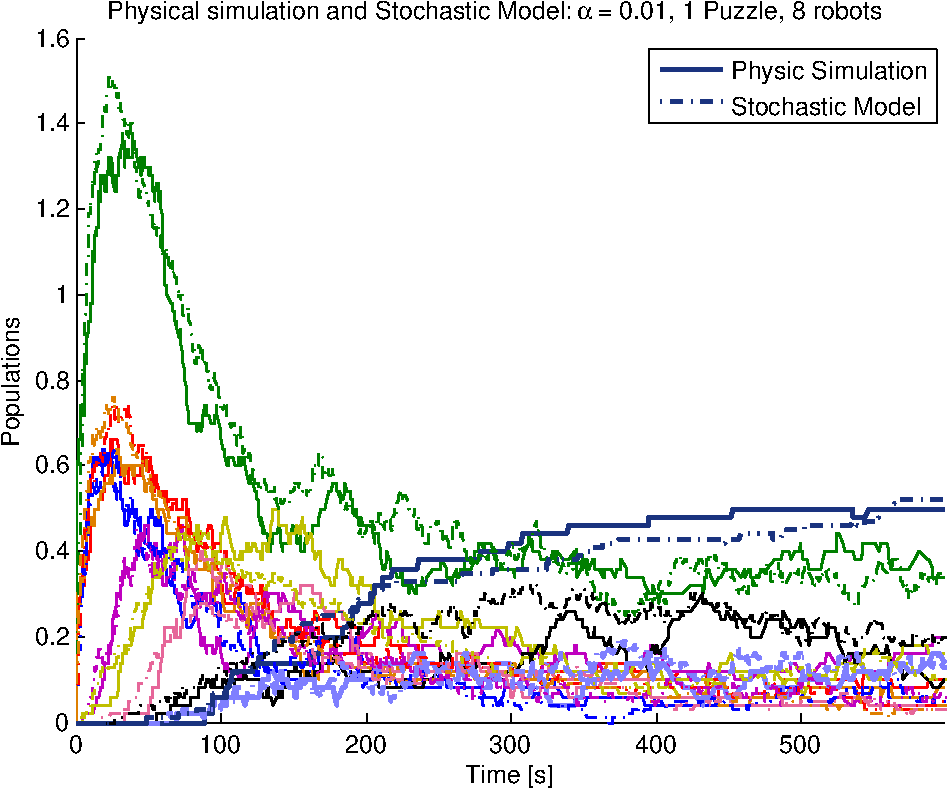
\includegraphics[width=10cm]{img/augm_stochphys_alpha001.pdf}
			\caption{Comparison between physical augmented system and stochastic model for $\alpha = 0.01$.}
			\label{fig:img_augm_stochphys_alpha001}
		\end{figure}
		
		The results between the physical and the stochastic simulations are comparable but differ slightly:
		
		\begin{my_itemize}
			\item The rates of convergence up to 9 minutes are of the same order. The stochastic model fits correctly the physical simulation.
			\item After 9 minutes, the stochastic model continues to converge towards its equilibrium, as expected from Figure~\ref{fig:stoch_augm_1puzzle:alpha001}, but the physical simulation saturates to a sub-optimal value. The amount of free pieces 2 is kept pretty high, without assembling to create the desired final puzzle F2. 
		\end{my_itemize}
		
		When observing visually the behavior of the system, it appears that two scenarios are occurring:
		\begin{my_enumerate}
			\item The system builds a final puzzle F2. As the backward rate from this puzzle is very slow, it is kept complete till the end of the simulation.
			\item The system builds a final puzzle F1. According to our rates, it should disassemble back till a convergence to F2. Unfortunately this disassembly does not work that well. Several problem arise:
				\begin{my_itemize}
					\item When F1 disassemble, it is very likely that the lying free piece 2 is taken and assembled back into a new F1. The problem comes from spatial constraints: the piece is dropped near the current robot.
					\item If F1 disassembles, we end up with an assembly 7 and an initial piece 2. The backward rate to disassemble 7 is low, which posses a problem in our case. We think that because 7 stays alive for some time, it has more chances to assemble back with the piece 2 than disassemble further, because of the spatial problem we presented.
				\end{my_itemize}
		\end{my_enumerate}
		
		There seems to be an even distribution between the two scenarios, the second of them impeding the capacity of the system to converge to the target ratio. We would need to do an iterative process to bring back this difference to the model level, in order to get optimized rates taking it into account.
		% subsubsection the_carried_pieces_discrepancy (end)
		
		\subsubsection{Other target ratios $\alpha$} % (fold)
		\label{ssub:other_target_ratios_alpha_}

			
			See Figure~\ref{fig:img_augm_stochphys_otheralpha} for the two other target ratio and their comparison with the stochastic model. The methodology is again the same, we perform 100 experiments of 20 minutes.
			
			We see that we closely fit the predicted data, but that the physical simulations converge to sub-optimal values in both cases. Again the ``mobility'' between assemblies in the real system is much smaller than in the model. This prevents a good convergence to theoretical values over time.
			
			
				\begin{figure}[h!]
					\centering
					\subfigure[$\alpha = 0.5$] 
					{
						\includegraphics[width=10cm]{img/augm_stochphys_alpha05.pdf}
						\label{fig:img_augm_stochphys_otheralpha:alpha05}
				 	}
			%		\: % espacement entre figures. \quad \;
					\subfigure[$\alpha = 0.99$] 
					{
						\includegraphics[width=10cm]{img/augm_stochphys_alpha099.pdf}
						\label{fig:img_augm_stochphys_otheralpha:alpha099}
				 	}
			%		\: % espacement entre figures. \quad \;
					\caption{Augmented system results for $\alpha=0.5$ and $\alpha=0.99$. Comparison with the stochastic model.}
				\label{fig:img_augm_stochphys_otheralpha} %Caption general
				\end{figure}
				
			Even though the yield is bad, it has to be remarked that the ratios $\alpha$ are successfully enforced by the optimized rates. This might point out that the problem does not come from the dynamics directly but from the small amount of pieces available. Further tests with bigger amount of pieces would be needed, but we are limited by simulation constraints for the time being.
			
		% subsubsection other_target_ratios_alpha_ (end)
	% subsection physical_simulation (end)
	
	\subsection{Implications} % (fold)
	\label{sub:implications}
		We saw that it was possible to use the rates we optimized in a simplified mathematical model to map onto the physical system. It successfully created the desired ratios of final puzzles, even though the dynamics of interactions between robots is quite complex and random. The Top-down approach of our framework is thus valid and promising even at this early stage.
		
		However, some differences can have big impacts. Small copy numbers can disturb the convergence, and the non-spatiality assumption can have bad effects when our physical system does not manage to satisfy it. We think that our approach is still worthy of interest and leads to insightful results, especially theoretically. It would need some tuning in order to map correctly the theoretical optimized probabilities onto the physical system. Unfortunately, this would have to be done in a further work.
	% subsection implications (end)
% section augmentation_results_and_implications (end)
% chapter augmented_assembly_implementation (end)Î

% % empty page
\pagebreak
\thispagestyle{empty}
\begin{center}\tiny \sc This page intentionally left blank.\end{center}
\pagebreak


\chapter{Conclusion and outlook} % (fold)
\label{cha:conclusion_and_outlook}
	\section{Conclusion} % (fold)
\label{sec:conclusion}
	Through this project, we presented a framework to perform a Top-down control over an existing system. It has been tested on a specific assembly task for robots.
	
	We first stated the overall framework and its components. Particularly, we defined two separate systems connected together by the Top-down control approach, the \textit{intrinsic} and the \textit{augmented} system. Our other major choice is the use of a Chemical Reaction Network mathematical model for all the framework. It allows a description of many systems while being widely accepted and used in the scientific community, especially in the life science community.

	\paragraph{}	
	We presented the test case on which we have applied our framework. This test case is a robotic assembly platform using a team of multiple robots. This has been completely developed and simulated using the 3D realistic physical simulation Webots. The platform has been created to verify a couple of properties, e.g. a well-mixed property of agents. The robotic platform allows us to assemble pieces following an arbitrary assembly plan, easily modifiable. We measured extensively the behavior of this platform under several conditions.
	
	\paragraph{}
	We introduced the mathematical representation in term of a chemical reaction network of our robotic platform. All its parameters where fitted by using first an heuristic guess based on geometric probabilities, behavior of the robots and measures of our platform. The theoretical parameters were then compared and adapted to the real measured ones, in order to closely fit to the physical simulation. This chemical reaction network has be simulated in two different ways: using an ODE approximation and with an exact stochastic simulation. Both simulations successfully captured the behavior of the physical system. The ODE approximation is wrong when few number of robots and pieces are considered, as one would hypothesize. On the other hand, the stochastic simulation captured especially well the quantitative global behavior of the physical system. Some characteristics still need to be accounted for, for example the irrecoverable errors in the physical simulation, or the divergence from a well-mixed system when the robots overcrowded certain parts of the arena.

	We also successfully modeled a scenario where the robotic platform can create two different final assemblies. The assembly plans used, as well as geometric constraints and pieces availability then defined the probability to generate the first or the second final assembly.
	
	\paragraph{}
	We introduced our Top-down control goal as the capacity to accurately control the ratio between the two final assemblies, while converging quickly to that state.
	
	In order to perform this control optimization, we introduced several results for the convergence of chemical networks and their dependence upon the reactions rate constants. We developed an algorithm representing the chemical reaction network and the goal of controlling the final ratio of final assemblies as a linear program function of the rate constants.
	
	It allowed us to define any target ratio and to make the system converge to it only by using a specific set of reactions rate constants. Control of the ratio was achieved by modifying only a small subset of all rates, namely the one controlling the final building reactions. The obtained behavior gave insights into the flexibility shown by such chemical reaction networks. We studied extensively the evolution of the controlled system and the behavior it showed. We then presented a direct application of our findings, in the shape of a ``green manufacturing'' system, which change its target final assembly smoothly during one experiment. It showed that our robotic platform displayed a flexibility in its capacities that are harder to replicate using classical assembly lines process for example.
	
	We finished by studying the effect of our optimization scheme on a set of assembly plans. The goal was to study if it would directly perform a discrete optimization of the plans, outputting the assembly plans most adapted to the assemblies being built. Interestingly, such a result took place, in a continuous fashion. A close analysis of the optimized rates showed several regimes of activity, corresponding to several dynamic plans, depending on the target assemblies. This is a surprising result, and research in that direction could lead to interesting discoveries.
	
	\paragraph{}
	Finally, we implemented our theoretical findings into our simulated robotic platform. This mapping was straightforward because of the strong relation built through the application of our whole framework. Stochastic simulations of the controlled system showed a behavior in accordance with the theoretical findings, even though several approximations were made to perform the optimization.
	
	However, the physical simulations showed a bigger discrepancy. The number of final puzzle was small and the system was crowded by initial and mid-assemblies. We think this is due to physical characteristics of our system, and because of the non-spatiality assumption made in the model. The real system does not validate this non-spatiality assumption in general, especially when disassembling a piece. This leads to a sub-optimal behavior when the number of pieces is too small.
	
	It showed that the last step in our framework, namely mapping back the model onto the physical system, is crucial, and very sensitive to hypotheses and real problems. It is still interesting to see that a full loop was successfully constructed, which would permit us to perform an iterative improving loop to more closely match the model to the physical system.

	\paragraph{}
	We think that our framework showed promising results, especially its model component. Chemical reaction networks are powerful explanatory tools, and they allow for a very precise yet very insightful representation of processes. While still being hard to manipulate and design because of their non linearity, we managed to propose an efficient optimization scheme, allowing a direct Top-down control scheme over the assembly process.
	
% section conclusion (end)

\section{Outlook} % (fold)
\label{sec:outlook}

	Further work might go in several directions:
	
	\begin{my_enumerate}
		\item A more precise and general way to map the mathematical model on the physical system, the Top-down mapping, should be proposed. As of now, we take advantage of the simplicity and strong links between our simulation and our model, but this might not be true for other systems. Furthermore, we saw that, even in our simple case, small problems could cause big issues.
		\item We created different assembly platforms, namely a self-assembly and a mixed-assembly platform. They showed interesting results, but were not studied mathematically and optimized in this current work. We think they might show new dynamics which would help improving our framework.
		\item Our optimization process should be verified and compared more thoroughly against other optimization and searches in the parameter space of possible rate constants. This is the goal of an ongoing paper on our work.
	\end{my_enumerate}
	
	Finally, we would really like to apply this framework to a completely different system, like a biological system or a microscale assembly process. Such systems show complex dynamics which requires a precise and flexible framework. As we first thought our framework to be applied to such systems, it would be only fair to eventually answer our claim that it is well adapted to such inherently complex systems.
	
	If this comes to be true, we would be pleased to have developed with success a framework capable of handling systems so utterly different as a biological process and a team of multi robots. We think there will be a need for flexible frameworks allowing an easy transfer of knowledge and informations between scientists working on completely different fields. Scientific work done at the frontier of several fields will soon give rise to impressive new possibilities (e.g. nanoscale robots to deliver drugs directly in the body), so if a framework can help towards that goal, we hope our work will provide a step forward.
	
% section outlook (end)
% chapter conclusion_and_outlook (end)

\chapter{Additional Material} % (fold)
\label{cha:additional_material}
	\section{Videos} % (fold)
\label{sec:videos}
	Videos showing the behavior of the robotic platform, for different scenarios and initial conditions, are available in the project's electronic handout.
% section videos (end)

\section{Acknowledgement} % (fold)
\label{sec:acknowledgement}
	
	I would like to especially thanks and acknowledge:\\
	Spring Berman for all her help, unbridled overnights and weekend hours of work and for abiding my unrestrained blattering.\\
	Gregory Mermoud for the help, support and lengthy discussions on world-changing discoveries.\\
	Prof. Vijay Kumar for his direction, availability and enthusiasm for this project.\\
	Prof. Alcherio Martinoli for his support and the given opportunity to discover a new culture and work in a great university.

	\paragraph{}
	\noindent And all the great people I've met at International House, who made me like the whole world a bit more.
	
% section acknowledgement (end)
% chapter additional_material_and_bibliography (end)


%%
%%  Bibliography
%%
\cleardoublepage
\addcontentsline{toc}{chapter}{{Bibliography}}

% Prints all the non-cited references
\nocite{*}

% Use style 'alphakey' or 'alpha' for the draft, and then switch
% to 'unsrt' or 'plain' or 'ieeetr' styles for the final version,
% since they are the IEEE preferred ones.
\bibliographystyle{ieeetr}
\bibliography{master_bib}


\end{document}